\documentclass[ms,electronic,twosidetoc,letterpaper,chaptercenter,parttop,lof,lot]{byumsphd}
% Author: Chris Monson
%
% This document is in the public domain
%
% Options for this class include the following (* indicates default):
%
%   phd (*) -- produce a dissertation
%   ms -- produce a thesis
%
%   electronic -- default official university option, overrides the following:
%                 - equalmargins
%
%   hardcopy -- overrides the following:
%                 - no equalmargins
%                 - twoside
%
%   letterpaper -- ignored, but helpful for the Makefile that I use
%
%   10pt -- 10 point font size
%   11pt -- 11 point font size
%   12pt (*) -- 12 point font size
%
%   lof -- produce a list of figures in the preamble (off)
%   lot -- produce a list of tables in the preamble (off)
%   lol -- produce a list of listings in the preamble (off)
%
%   layout -- show layout lines on the pages, helps with overfull boxes (off)
%   grid -- show a half-inch grid on every page, helps with printing (off)
%   separator -- print an extra instruction page between preamble and body (off)
%
%   twoside (*) -- two-sided output (margins alternate for odd and even pages,
%     blank pages inserted to ensure that chapters begin on the right side of a
%     bound copy, etc.)
%   oneside -- one-sided output (margins are the same on all pages)
%   equalmargins -- make all margins equal - ugly for binding, but compliant
%
%   twosidetoc - start two-sided margins at the TOC instead of the body.  This
%     is sometimes (oddly) required, but be aware that it will make the page
%     numbering seem screwy, e.g., the first four full sheets of paper will
%     have number i-iv (not shown, though), and the next sheets will each have
%     two numbers, one for each side.  I suspect that most people don't look at
%     the roman numerals anyway, but it is a weird requirement.
%
%   openright (*) -- force new chapters to start on an odd page
%   openany -- don't use this, it's ugly
%
%   prettyheadings -- make the section/chapter headings look nice
%   compliantheadings (*) -- make them look ugly, but compliant with standards
%
%   chaptercenter -- center the chapter headings horizontally
%   chapterleft (*) -- place chapter headings on the left
%
%   partmiddle -- Part headers are centered vertically, no other text on page
%   parttop (*) -- Part headers at top of page, other text expected
%
%   duplexprinter -- Ensures that the two-sided portion starts on the right
%     side when printing.  This is not for use in submission, since the best
%     thing to do there is to print everything out one-sided, then take it down
%     to the copy store to have them do the rest.  It does help to save trees
%     when you are printing out copies just to look at them and fiddle with
%     things.
%
%
% EXAMPLES:
%
% The rest is up to you.  To fiddle with margins, use the \settextwidth and
% \setbindingoffset macros, described below.  I suggest that you
% \settextwidth{6.0in} for better-looking output (otherwise you'll get 3/4-inch
% margins after binding, which is sort of weird).  This will depend on the
% opinions of the various dean/coordinator folks, though, so be sure to ask
% them before embarking on a major formatting task.

% The following command fixes my particular printer, which starts 0.03 inches
% too low, shifting the whole page down by that amount.  This shifts the
% document content up so that it comes out right when printed.
%
% Discovering this sort of behavior is best done by specifying the ``grid''
% option in the class parameters above.  It prints a 1/2 inch grid on every
% page.  You can then use a ruler to determine exactly what the printer is
% doing.
%
% Uncomment to shift content up (accounting for printer problems)
%\setlength{\voffset}{-.03in}

% Here we set things up for invisible hyperlinks in the document.  This makes
% the electronic version clickable without changing the way that the document
% prints.  It's useful, but optional.
%
% NOTE: "driverfallback=ps2pdf" chooses ps2pdf in the case of LaTeX and pdftex
% in the case of pdflatex. If you use my LaTeX makefile (at
% http://latex-makefile.googlecode.com/) then pdftex is the default There are
% many other benefits to using the makefile, too.  This option is not always
% available, so use with care.
\usepackage[
    bookmarks=true,
    bookmarksnumbered=true,
    breaklinks=false,
    raiselinks=true,
    pdfborder={0 0 0},
    colorlinks=false,
    plainpages=false,
    ]{hyperref}

\usepackage{graphicx}
\usepackage{caption}
\usepackage{subcaption}
\usepackage{float}
\usepackage{scrextend}
\usepackage{url}
%\usepackage{courier}
\usepackage{titlesec}
\usepackage[]{algorithm2e}
\usepackage{amsmath}
\usepackage{titlesec}

\setcounter{secnumdepth}{4}

% To fiddle with the margin settings use the below.  DO NOT change stuff
% directly (like setting \textwidth) - it will break subtle things and you'll
% be tearing your hair out.
%
% For example, if you want 1.5in equal margins, or 2in and 1in margins when
% printing, add the following below:
%
%\setbindingoffset{1.0in}
%\settextwidth{5.5in}
%
% When equalmargins is specified in the class options, the margins will be
% equal at 1.5in each: (8.5 - 5.5) / 2.  When equalmargins is not specified,
% the inner margin will be 2.0 and the outer margin will be 1.0: inner = (8.5 -
% 5.5 - 1.0) / 2 + 1.0 (the 1.0 is the binding offset).
%
% The idea is this: you determine how much space the text is going to take up,
% whether for an electronic document (equalmargins) or not.  You don't want the
% layout shifting around between printed and electronic documents.
%
% So, you specify the text width.  Then, if there is a binding offset (when
% binding your thesis, the binding takes up space - usually 0.5 inches), that
% reduces the visual space on the final printed copy.  So, the *effective*
% margins are calculated by reducing the page size by the binding offset, then
% computing the remaining space and dividing by two.  Adding back in the
% binding offset gives the inner margin.  The outer margin is just what's left.
%
% All of this is done using the geometry package, which should be manipulated
% directly at your peril.  It's best just to use the above macros to manipulate
% your margins.
%
% That said, using the geometry macro to set top and bottom margins, or
% anything else vertical, is perfectly safe and encouraged, e.g.,
%
%\geometry{top=2.0in,bottom=2.0in}
%
% Just don't fiddle with horizontal margins this way.  You have been warned.

% This makes hyperlinks point to the tops of figures, not their captions
\usepackage[all]{hypcap}

% These packages allow the bibliography to be sorted alphabetically and allow references to more than one paper to be sorted and compressed (i.e. instead of [5,2,4,6] you get [2,4-6])
\usepackage[numbers,sort&compress]{natbib}
\usepackage{hypernat}

% Because I use these things in more than one place, I created new commands for
% them.  I did not use \providecommand because I absolutely want LaTeX to error
% out if these already exist.
\newcommand{\Title}{Subword Spotting and its Applications}
\newcommand{\Author}{Brian L.~Davis}
\newcommand{\GraduationMonth}{April}
\newcommand{\GraduationYear}{2018}

% Set up the internal PDF information so that it becomes part of the document
% metadata.  The pdfinfo command will display this.
\hypersetup{%
    pdftitle=\Title,%
    pdfauthor=\Author,%
    pdfsubject={MS Thesis, BYU CS Department: %
                Degree Granted \GraduationMonth~\GraduationYear, Document Created \today},%
    pdfkeywords={subword, spotting, CAT, semi-automated, handwriting},%
}

% Rewrite the itemize, description, and enumerate environments to have more
% reasonable spacing:
\newcommand{\ItemSep}{\itemsep 0pt}
\let\oldenum=\enumerate
\renewcommand{\enumerate}{\oldenum \ItemSep}
\let\olditem=\itemize
\renewcommand{\itemize}{\olditem \ItemSep}
\let\olddesc=\description
\renewcommand{\description}{\olddesc \ItemSep}

% Important settings for the byumsphd class.
\title{\Title}
\author{\Author}

\committeechair{William Barrett}
\committeemembera{Thomas Sederberg}
\committeememberb{Daniel Zappala}

\monthgraduated{\GraduationMonth}
\yeargraduated{\GraduationYear}
\yearcopyrighted{\GraduationYear}

\documentabstract{%
We propose subword spotting, a generalization of word spotting where the search may be for groups of characters within words. We present a method for performing subword spotting based on state-of-the-art word spotting techniques and evaluate its performance at three granularitires (unigrams, bigrams and trigrams) on two datasets.

We demonstrate three applications of subword spotting, though others may exits. The first is assisting human transcribers identify unrecognized characters by locating them in other words. The second is searching for suffixes directly in word images (suffix spotting). And the third is computer assisted transcription (semi-automated transcription). We investigate several variations of computer assisted transcription, but none achieve transcription speeds above manual transcription. We investigate the causes.
}

\documentkeywords{%
	subword, spotting, CAT, semi-automated, handwriting, n-gram, character
}

\acknowledgments{%
    I would like to thank my wife Sarah for her patience with and support of my endeavors.
    \\
    \\
    
    I would like to extend thanks to Curtis Wigington, Seth Stewart, Chris Tensmyer and Bill Barrett, who, among other assistance to my work, provided use timing data for my semi-autometed transcription system used in its simulations.
}

\department{Computer~Science}
\graduatecoordinator{Christophe Giraud-Carrier}
\collegedean{Shane~Reese}
\collegedeantitle{Dean}

% Customize the name of the Table of Contents section.
\renewcommand\contentsname{Table of Contents}

% Remove all widows an orphans.  This is not normally recommended, but in a
% paper dissertation there is no reasonable way around it; you can't exactly
% rewrite already-published content to fix the problem.
\clubpenalty 10000
\widowpenalty 10000

% Allow pages to have extra blank space at the bottom in order to accommodate
% removal of widows and orphans.
\raggedbottom

% Produce nicely formatted paragraphs. There is nothing additional to do.  In
% case you get some problems, surround your text with
% \begin{sloppy} ... \end{sloppy}. If that does not work, try
% \microtypesetup{protrusion=false} ... \microtypesetup{protrusion=true}
\usepackage{microtype}

\begin{document}

% Produce the preamble
\microtypesetup{protrusion=false}
\maketitle
\microtypesetup{protrusion=true}

%%%%%%%%%%%%%%%%%%%%%%%%%%%%%%%%%%%%%%%%%%%%%%%%%%%%%%%%%%%%%%%%%%%%%%%%%%%%%%
\chapter{Introduction}

Most data recorded by humans in the past, and much even today, is in handwritten documents. 
It is highly desirable for many areas of research for this information to be easily accessible, either being searchable through automatic means or having the data digitized in some form that is easily manipulated by computers.

The digitization of these documents is a large task. Obviously not all recorded data is important, but even within a specific domain, the number of relevant handwritten documents can be far too large to be manually transcribed to digital text (that is, a human reads the document and then types the contents into a computer). Within the domain of family history research there are billions of handwritten documents which have been photographed as digital images and more are being captured every day.
%which would be easily searchable if they were transcribed to digital text. Digitized records also can facilitate automated information extraction (e.g.~relationships between people for genealogical purposes). A mighty effort has been underway to capture many of these documents as digital images, but 
The transcription of these lags far behind, and the gap is growing. It is an expensive task to have the contents of these documents manually typed by people.

A solution to the problem of transcribing documents that has been worked on for several decades is automated handwriting recognition. The basic formulation is that given an image of handwriting (either a character, word, line, paragraph or page), automatically produce the text of its handwritten content. The state-of-the art is primarily focused on the transcription of text lines and paragraphs through artificial neural networks, particularly recursive neural networks (RNN) \cite{icfhrComp2016, wigington2017, icdarComp2017}. These methods work relatively well, particularly in single author scenarios. However, they do require large training sets and would require human correction in some difficult applications where human-level accuracy is required.

Computer assisted transcription (CAT), or semi-automated transcription, is an approach to transcription which begins with the understanding that human input will be needed to achieve the desired accuracy and aims to merge computed and human effort in an effective manner. 
These methods have generated less interest recently due to the large gains deep convolutional neural networks have given automatic transcription.

However, transcription is not always needed; if search is the only utility desired an alternative solution is word spotting \cite{manmatha1996}. In word spotting, the goal is to make a collection of document images searchable without transcription. The search results are based on visual features the system extracts. The result of word spotting is the location, and potentially bounding box, of all instances of the query (see Figure \ref{fig:explain_spotting}). 

\begin{figure}[t]
    \begin{subfigure}{0.46\textwidth}
    		\centering
    		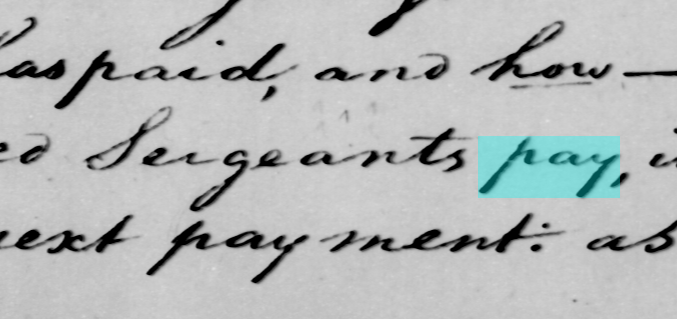
\includegraphics[width=\textwidth]{spotting_explination_pay}
    		%\caption{A small window shows the user matching words later in the column. The user can get rid of bad matches by either clicking on them or adjusting a  threshold.}
    	\end{subfigure}
    	~
    	\begin{subfigure}{0.46\textwidth}
    		\centering
    		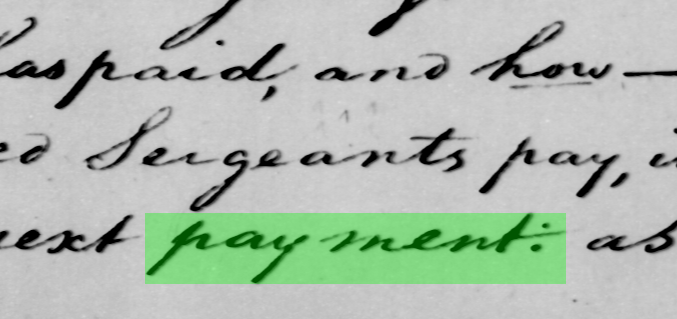
\includegraphics[width=\textwidth]{spotting_explination_payment}
    		%\caption{The matched words are given the same label when entered.}
    	\end{subfigure}
    	\caption{Examples of word spotting for `pay' and `payment'.}
    	\label{fig:explain_spotting}
\end{figure}

\begin{figure}[t]
    \begin{subfigure}{0.46\textwidth}
    		\centering
    		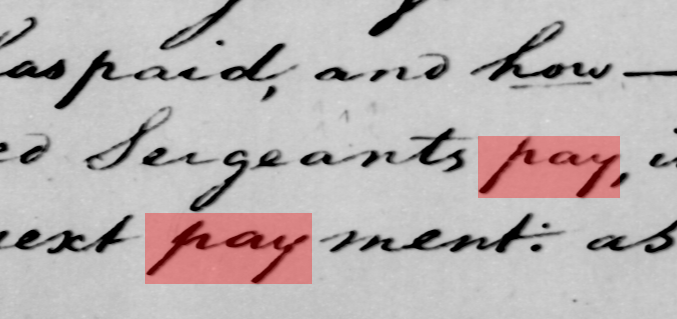
\includegraphics[width=\textwidth]{spotting_explination_sub_pay}
    		%\caption{A small window shows the user matching words later in the column. The user can get rid of bad matches by either clicking on them or adjusting a  threshold.}
    	\end{subfigure}
    	~
    	\begin{subfigure}{0.46\textwidth}
    		\centering
    		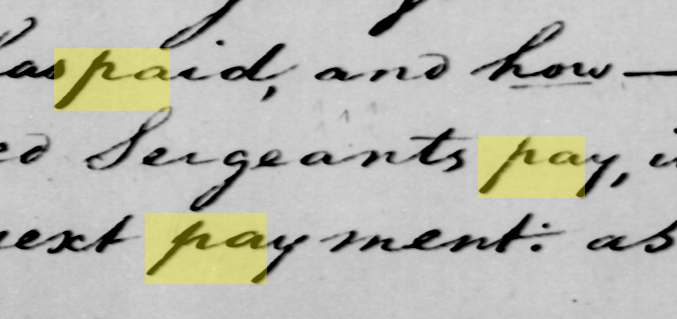
\includegraphics[width=\textwidth]{spotting_explination_sub_pa}
    		%\caption{The matched words are given the same label when entered.}
    	\end{subfigure}
    	\caption{Examples of subword spotting for the character trigram `pay' (left, red) and bigram `pa' (right, yellow).}
    	\label{fig:explain_sub_spotting}
\end{figure}

In this work, subword spotting is explored. Where word spotting finds words matching a query, subword spotting relaxes this to finding any instances of the query, even within a word. As seen in Figure \ref{fig:explain_sub_spotting} (left, red), an additional instance of ``pay'' is found compared to Figure \ref{fig:explain_spotting}.
And in Figure \ref{fig:explain_sub_spotting} (right, yellow), an additional instance of ``pa'' is found, which turns out to be a different form of the word``pay''.
%Of interest in subword spotting are atomic units of words which occur...



%The scope of this thesis is to use subword spotting (looking for groups of characters within words) as the back-bone of a CAT system. This aims to break the transcription task, from a user perspective, to micro-tasks that can be completed easily with a smartphone. For any CAT system to be considered successful, it must be faster than manual transcription while achieving comparable accuracy.

\section{Why Subword Spotting?}

The original motivation for exploring subword spotting came from the observation that techniques for handwriting recognition have tried many different primitives, or fundamental units, for recognition. One can look at pixels at the lowest level, and then move onto graphemes or substrokes \cite{liang2012}, strokes, characters, subwords (or character n-grams), words and sentences. With current neural networks, the primitives are learned within the stacked convolutional layers, and the network then recognizes characters based on these. Previous CAT systems such as \cite{Clawson2014} and \cite{Zagoris2015} use whole words as units for recognition. 

%Subwords provide an interesting middle ground between these units. Characters can be very similar to one another (in cursive ``i'' missing it's dot frequently looks like an ``e'') making discriminating between them very difficult. Words, on the other hand, can occur very infrequently, such as names which occur once in an entire corpus. Subwords occur frequently while providing more context than single characters and thus may be a primitive well suited to handwritting.


An individual primitive has two desirable properties: distinctiveness and frequency. Without distinctiveness it will be very difficult to discriminate between different primitive instances. Frequency is valuable as it allows us to get more out of the effort required to discriminate, or potentially the effort required to learn how to discriminate.

Subwords provide an interesting middle ground between individual characters and complete words. %, each of these having flaws improved upon by subwords.
Individual characters can be very similar to one another (i.e.~not distinctive). For example, in cursive an ``i'' missing it's dot frequently looks like an ``e'', as seen in Figure \ref{fig:ei}, making discriminating between characters in isolation very difficult. On the other hand, words are generally much more distinctive than characters. However, while individual characters occur many times throughout a corpus, a given word may appear less frequently. In the extreme, words such as names, may occur only once. However, subwords, such as ``th'', ``ed'', ``ion'', ``ing'', etc., occur very frequently (in English) as they are used in many words. And while being more frequent than words, subwords also provide more distinctiveness and discernibility than individual characters.

\begin{figure}
    \centering
    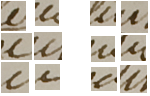
\includegraphics[width=0.45\textwidth]{ei}
    \caption{Cropped examples of the characters ``e'' and ``i'' (excluding dots), on the left and right respectively, from a single author. Without context the characters are practically indistinguishable.}
    \label{fig:ei}
\end{figure}

Important use cases for subword spotting include searches (1) where a root is desired to be searched, such as querying ``pay'' wanting to find instances of ``payment'', ``payments'', ``prepay'', etc., (2) where only part of the desired word, such as a name, is known, such as ``Chr.'', (3) where there are character(s) which a human transcriber cannot initially recognize, but if instances elsewhere in the document in familiar words could be found in context, would become discernible to the transcriber.

An additional appeal of subword spotting lies in computer assisted transcription (CAT). In character-level recognition schemes, a lexicon is frequently used to correct erroneous character predictions if other characters in the word are transcribed correctly. Similarly a lexicon can also be used to fill in untranscribed characters, assuming significant other characters are transcribed. This is useful in a transcription by iteratively spotting subwords. While the spotting results may not cover every character, they can cover a sufficient number of characters for each particular word.

In Figure \ref{fig:subtransexample} we see an example of the word ``payment'', where ``pa'' and ``men'' have been spotted; this covers 71\% of the characters in the word. However, if we estimate that there are 1-2 characters between ``pa'' and ``men'' and estimate 1-2 characters after ``men'' the regular expression \texttt{pa..?men..?} matchs only ``pavement'', ``pavements'', ``payment'', and ``payments'' in our large lexicon (described in Chapter \ref{datasets}). This is a particularly potent tool with longer words, which typically may require more effort to automatically transcribe, but tend to be more distinctive from a lexical perspective.

\begin{figure}
    \centering
    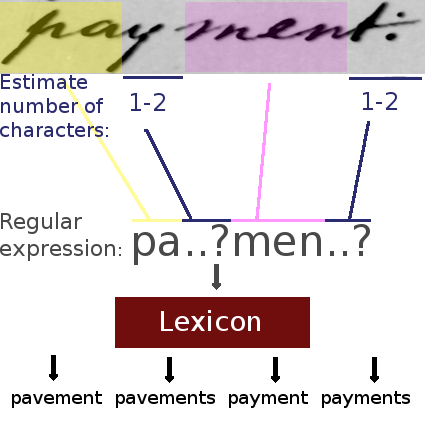
\includegraphics[width=0.55\textwidth]{spotting_completion_payment}
    \caption{An example of a word having ``pa'' and ``men'' spotted in it. A regular expression representing this, \texttt{pa..?men..?}, yields only a few matches from our lexicon, including the correct one: ``pavement'', ``pavements'', ``\textbf{payment}'', and ``payments''.}
    \label{fig:subtransexample}
\end{figure}

%While these previous motivations are based on transcription, subword spotting has a the potential to be a more flexible search tool than word spotting is. In this work we show this in the application of searching for words with specific suffixes.

\section{Main Contributions}

The primary scope of this work is to provide an exploration of the performance of subword spotting, extending state-of-the-art word spotting methods.
We show that reasonable levels of mean average precision (MAP) can be achieved for character tri-, bi-, and unigram spotting. We demonstrate the variability in performance between different character n-grams (referred to simply as n-grams hereafter).

Additionally, we demonstrate several applications of subword spotting: user directed searching to aid in human transcription, suffix searching/spotting, and CAT using word completion from aggregated subword spottings.

%%%%%%%%%%%%%%%%%%%%%%%%%%%%%%%%%%%%%%%%%%%%%%%%%%%%%%%%%%%%%%%%%%%%%%%%%%%%%%
\chapter{Related Work}\label{relatedwork}

\section{Word Spotting}\label{relatedwork_wordspotting}


Word spotting was first proposed as an alternative to transcribing a corpus. Rather than transcribing the document image so standard text searches can be run, the document is searched using the images themselves, either with a keyword string or a keyword image (exemplar image). In the past, techniques were distinguished by which search pattern they used. There are two primary approaches to featurizing the images when word spotting is performed: holistic features, that capture information about a whole image (word), and local or sequential features \cite{Rodrıguez2008}. Holistic features have one description for an entire word image (such as a bag-of-visual-words \cite{Shekhar2012}), whereas local features have a descriptor for a small portion, or window, of a word image. 
%Because local features provide much more detail and are more flexible than holistic features, they have been the most actively pursued in research.

Most early work with local features share the common theme of taking features from vertical slice windows (usually only one or a handful of pixels wide); Figure \ref{fig:vertslice} shows an example of this process. They compare these to the features extracted from an exemplar using either dynamic time warping or hidden Markov models (HMMs), relying on a prior line segmentation. The variation between the methods largely lies in the features used. Some use small square windows to allow segmentation-free word spotting using a sliding window \cite{Rothacker2013}.

\begin{figure}[t]
    \centering
    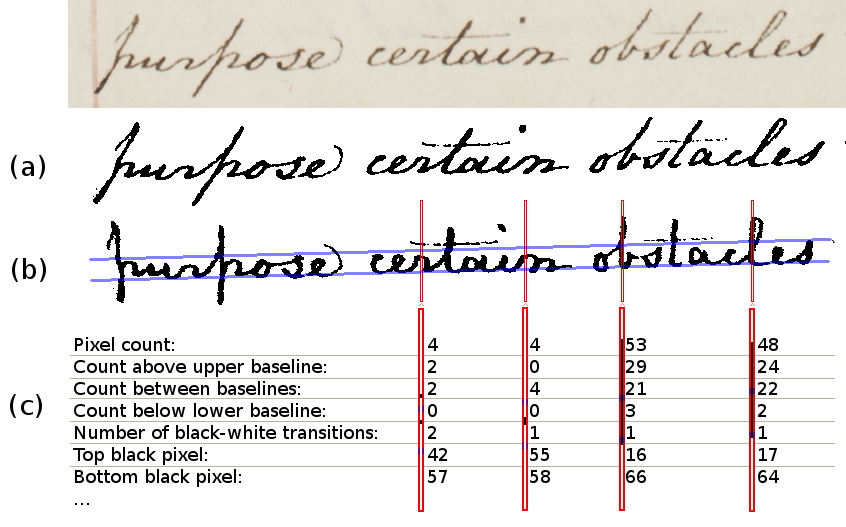
\includegraphics[width=.99\textwidth]{vertwind}
    \caption{Example of how vertical slice window features are extracted. Typically most features are extracted on a binarized image (a). Deskewing the image (b) plays an important role as the vertical slices are very sensitive to skew. Many typical features extracted (c) are pixel counts; in this example we show count features dependent on baselines (blue).}
    \label{fig:vertslice}
\end{figure}

Rodr{\i}guez et al.~\cite{Rodrıguez2008} proposed a simple histogram gradient feature that demonstrated improved performance when compared with (1) the popular profile and transition-based features of Rath and Manmantha \cite{Rath2003}, (2) the gradient and transition-focused features of Marti and Bunke \cite{Marti2001} and (3) the simple histogram features of Bunke et al.~\cite{Bunke2004}. They also showed that a HMM worked better than dynamic time warping, for their features. Their method was not an exemplar-based approach.

Aldavert et al.~\cite{Aldavert2015} and Almazan et al.~\cite{Almazan2014} have presented superior word spotting methods that rely on heuristic descriptions. Aldavert et al.~used the well known bag-of-visual-words method, including recent improvements from the computer vision community. This is a very simple, yet effective, exemplar spotting approach. Aldavert et al.~use Fischer vectors, which are similar to bag-of-visual-words, with spatial pyramids in addition to a special pyramidal histogram of characters (PHOC).
% which are described in more detail in Chapter \ref{subwordspott`ing}. 
PHOC vectors are a fixed length vector which describe a word; it encodes which characters are present and roughly their location. If your alphabet is length $N$, the first $N$ values of the vector indicate if each character is present in the word (Is `a' in the word? Is `b' in the word?). The next $N$ values indicate if each character is present in the first half of the word, the $N$ values after that indicating presence in the second half of the word (this is the rough location encoding). This is carried out to three levels. In the original PHOC a set of character bigrams are also used on the first two levels, however, we do not use these. See Figure \ref{fig:phoc} for clarification.
The PHOC vector and pyramidal bag-of-visual-words are used to find a new space in training in which both strings and word images can be embedded. This allows it to perform both string and exemplar queries as well as hybrid queries which yield excellent results.

\begin{figure}[t]
    \centering
    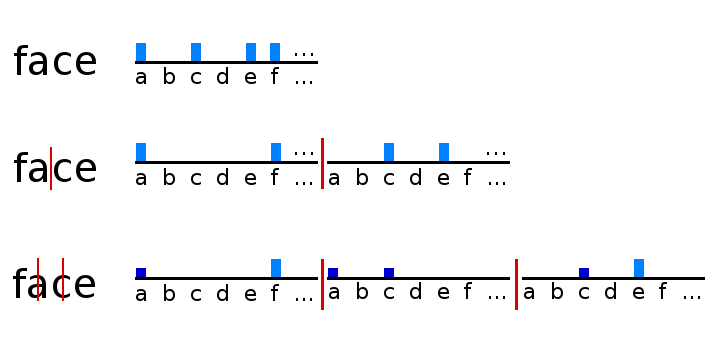
\includegraphics[width=.65\textwidth]{phoc}
    \caption{Example of a three-level PHOC vector for the word ``face''. The final vector is all levels appended together. Note that partial values are given when characters are split over bins.}
    \label{fig:phoc}
\end{figure}

%PHOCNet
Sudholt and Fink \cite{sudholt2016,sudholt2017} expanded on \cite{Almazan2014} by training a deep convolutional neural network to produce the PHOC vector from a word image. This, and following improvements \cite{krishnan2016, retsinasTrans2017}, have yielded the state-of-the-art for segmentation based spotting. We base our spotting method on \cite{sudholt2017}.

There are also techniques for segmentation-free word spotting, where spotting is performed on a full page without any segmentation information \cite{wilkinson2017}. While we used word image segmentations in our work to narrow its scope, we note that it could be applied, with some adjustments, in a segmentation-free setting.

In this thesis we are interested in spotting character n-grams (uni-, bi- and trigrams) rather than words. While this hasn't explicitly been done, we feel examining the performance of other methods on short words (2 to 3 letters) is instructive. For Rothacker et al.'s \cite{Rothacker2013} segmentation-free HMM based method, they report $\sim$46\% and $\sim$55\% mean Average Precision (mAP) for two- and three-lettered words respectively, a drop by $\sim$15\% and $\sim$6\% from the mAP for all words they tested (61\%). Fischer et al.~\cite{Fischer2012} report $\sim$70\% and $\sim$83\% mAP for two and three lettered words, compared to {\textgreater}90\% mAP for words of length 5 or longer, for their line segmentation dependent, character HMM based method. While neither of these numbers are very promising, Almazan et al.~\cite{Almazan2012} observe that sliding window approaches can frequently find false positives of short words inside other words (e.g.~finding the word ``the'' inside the word ``weather''). As this is precisely what we want to have happen in n-gram spotting (that is, we \textit{want} to find groups of letters in the middle of words), we expect we should have more success spotting character n-grams than other methods in spotting short words, assuming we have good sliding windows. However, part of the poor accuracy in spotting short words is simply the fact that there is less information with which to discriminate.%; this is an obstacle we still must overcome.

%Closely related to subword spotting is glyph spotting, where single characters are searched for; typically in languages where single characters carry more meaning than English.

\section{Automatic Handwriting Recognition}

%[!] Should this be here, or only in introduction?
The state-of-the-art for handwriting recognition relies heavily on recursive neural networks (RNNs) paired with convolutional neural networks (CNNs). The key component is the connectionist temporal classification (CTC) loss which allows the network to be trained given a line image and the ground truth text for that line without any alignment \cite{CTC}. In a recent competition on historical German documents \cite{icdarComp2017} (see Figure \ref{fig:germanlines}), the leading contestants used a bidirectional RNN on top of a CNN. The best results had word error rates of 19.1\% and character error rates of 7.0\%. This is impressively low given the diversity of the data, and deep learning methods are continuing to improve \cite{wigington2017,puigcerver2017}.

\begin{figure}[t]
    \centering
    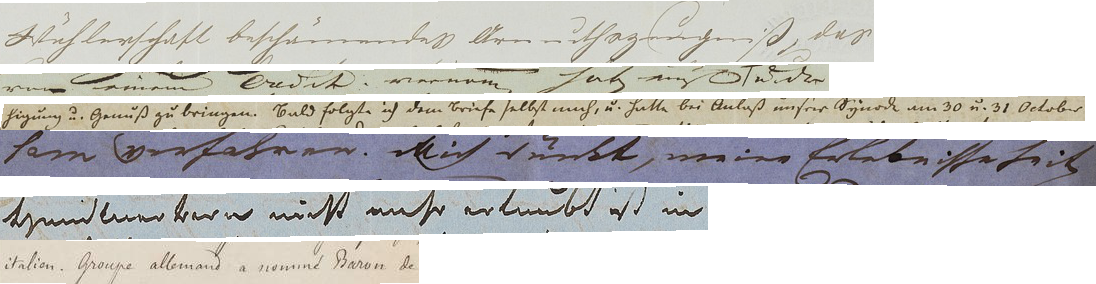
\includegraphics[width=.98\textwidth]{german_lines}
    \caption{Example of lines extracted from the dataset of the ICDAR HTR competition \cite{icdarComp2017}.}
    \label{fig:germanlines}
\end{figure}

%copied from proposal [!]

\section{Computer Assisted Transcription} %TODO, brand corrective/directive

%Due to the limitations of current handwriting recognition methods, we believe that a fully automated handwriting transcription is out of reach with the present of technology. We thus turn our attention to semi-automated recognition approaches, where we are still using a human to transcribe, but also some intelligent recognition technology. A semi-automated solution will outperform a fully automated system in terms of accuracy and is still far more effective than completely manual transcription. 
There tends to be two primary CAT (Computer Assisted Transcription) methodologies: corrective and directive. Corrective CAT methods rely on handwriting recognition to do most of the work, and then users provide feedback correcting some errors of the recognition, where the gain comes from other errors being automatically corrected or being assisted so that corrections are easier to make.

In a directive CAT method, the user provides some of the initial input to the system and it uses this to transcribe more than what the user inputted.
%Standard CAT approaches use human feedback in two ways: to correct or direct. Either the user is correcting automatic transcription in an intelligent way, or to seeding and directing the recognition by labeling/transcribing words.
%Both try two use human input in an intelligent way were more is learned than simply the label/correction given. 
An active learning approach to handwriting transcription is similar to CAT, but is not concerned about achieving human level accuracy, just better accuracy, and thus requires less human involvement~\cite{Serrano2010}. 
%Since we wish to have a system with accuracy comparable to human performance, 
We will focus on CAT approaches.

Toselli et al.~\cite{Toselli2007} have explored the realm of corrective CAT using the idea of user-verified prefixes. They use a fairly standard HMM recognition model as the backbone of their approach, and take advantage of the incremental nature of the Viterbi decoding algorithm. The recognition is done for a line of text and the user corrects the first error. The Viterbi decoding is then run again, but this time using the assumption that everything occurring before the correction is correct, and thus reusing the computation up to that point. They have also explored slight variations of the same approach that enable more fluent user input with a touchpad \cite{Toselli2008}, mouse \cite{Toselli2009}, or multimodal means \cite{Toselli2010}, which speed up the transcription process by allowing more intuitive user interaction (Fig.~\ref{fig:Toselli_multimodalCAT}). Their approach relies on a language model to make corrections on a line when a supervision is made. This means this method cannot be used to effectively transcribe documents containing non-sentence writing, such as tables and lists. Serrano, et al.~also have pursued a similar approach, where the user corrects the \textit{n} words in which the recognition model had the least confidence \cite{Serrano2014}.

\begin{figure}
    \centering
    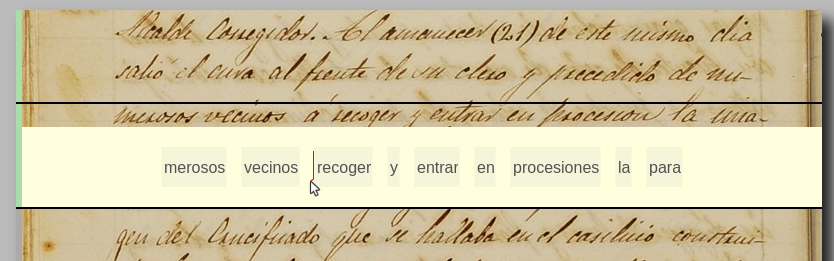
\includegraphics[width=0.95\textwidth]{Toselli_multimodalCAT}
    \caption{A screenshot of a demo of Toselli et al's multimodal CAT system. The red line is drawn by the user to indicate the need to insert a word into the automatically obtained transcription.}
    \label{fig:Toselli_multimodalCAT}
\end{figure}

While it is useful to employ an automatic handwriting recognition method as part of a CAT approach to reduce the human burden, we cannot use the same type of recognition used by these previous CAT systems, where there is a reliance on the predictive capacity of a language model. Some documents are not comprised of only sentences, and thus cannot be transcribed by these methods (e.g.~the name field of census documents, see Figure \ref{fig:ii}). However, many documents are structured such that a pattern can be learned to assist in transcription.


Robert Clawson \cite{Clawson2014}\footnote{You can view a short demo and explanation of his approach at \url{https://www.youtube.com/watch?v=gqdVzEPnBEw}} designed a CAT system for handwritten tabular documents, which have a clear pattern. His approach relies on simply finding matches in the document column of the current word image (red box in Figure \ref{fig:ii}(a). This is essentially query by example word spotting with user oversight. The matched words are assigned the same user-specified label. This provides an accurate CAT system where the user oversees all transcription. The user oversight of matches is accomplished by showing a list of matches to the user (with an adjustable threshold for sensitivity) from which the user removes the false-positive matches. The remaining all have the same label applied to them. This interface, discarding bad matches, leverages the human user's natural ability to quickly identify outliers.
Our CAT attempts to also leverage this ability as well.
%However, the approach as a whole is limited as it requires frequent word repetition to be effective. While some tabular documents have this, it is not true for most other documents. Additionally, this method required a computationally expensive preprocessing stage in which a similarity score of all words in a column with all other words in the column had to be computed.
%The word image comparison method used in \cite{Clawson2014} was costly and prohin

\begin{figure}
    \centering
    \begin{subfigure}[t]{0.46\textwidth}
    		\centering
    		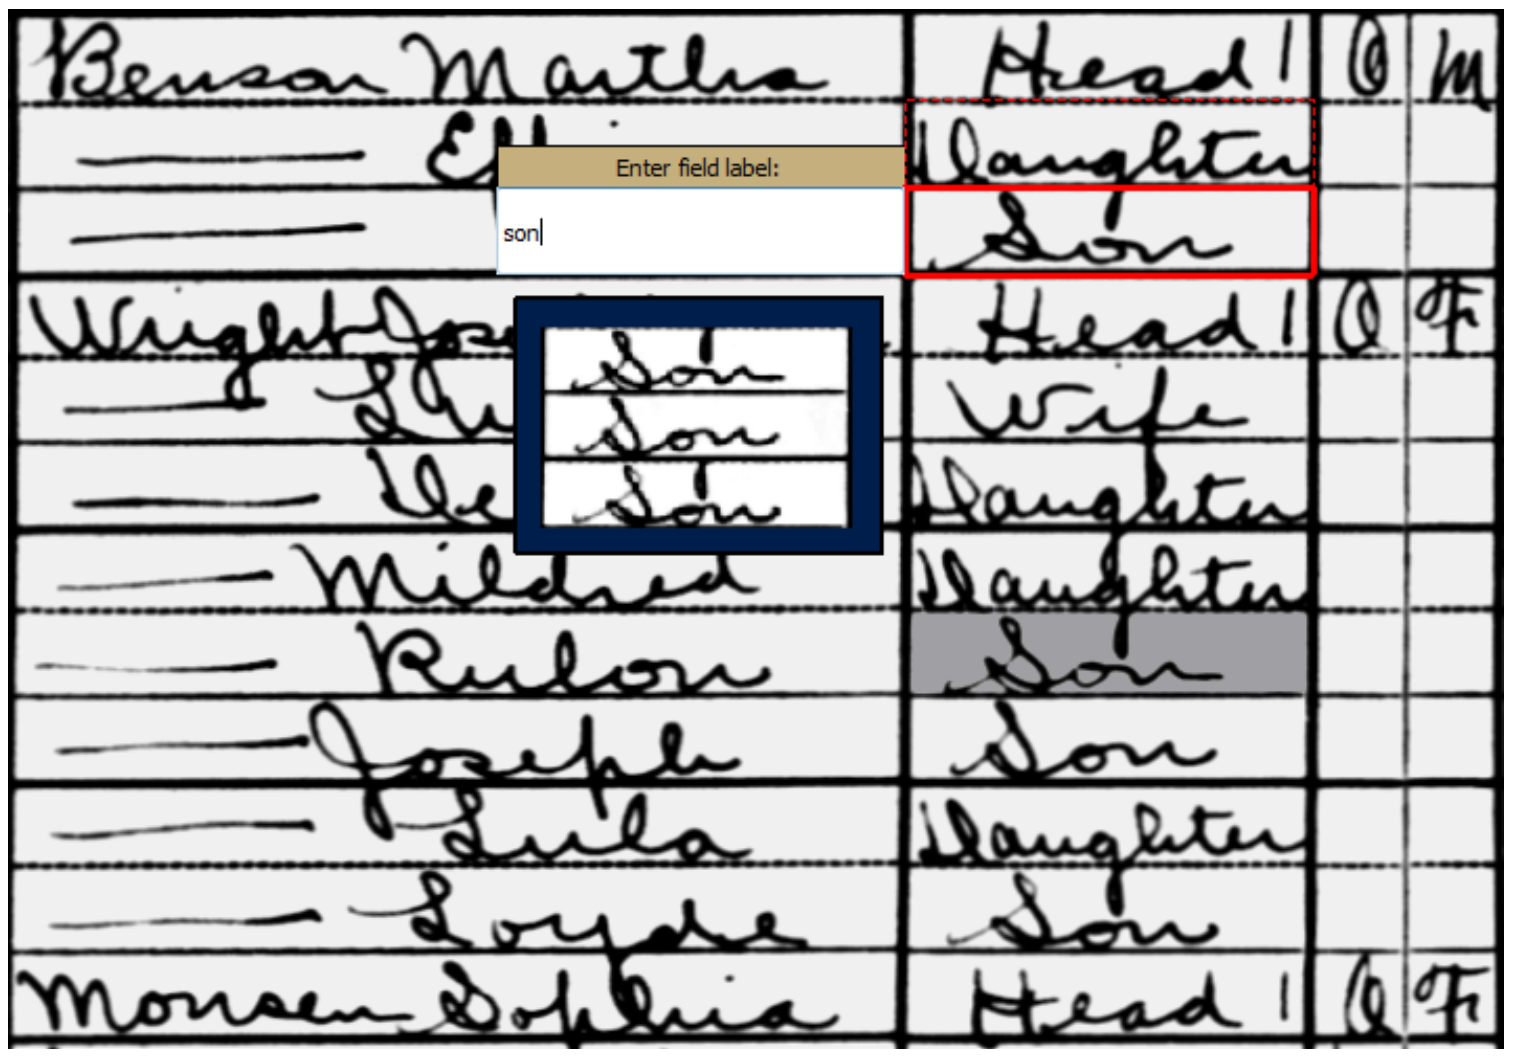
\includegraphics[width=\textwidth]{ii_ex_a}
    		\caption{The red box indicates the current word. A small window shows the matching words that appear elsewhere in the column. The user can get rid of bad matches by either clicking on them or adjusting a  threshold.}
    	\end{subfigure}
    	~
    	\begin{subfigure}[t]{0.46\textwidth}
    		\centering
    		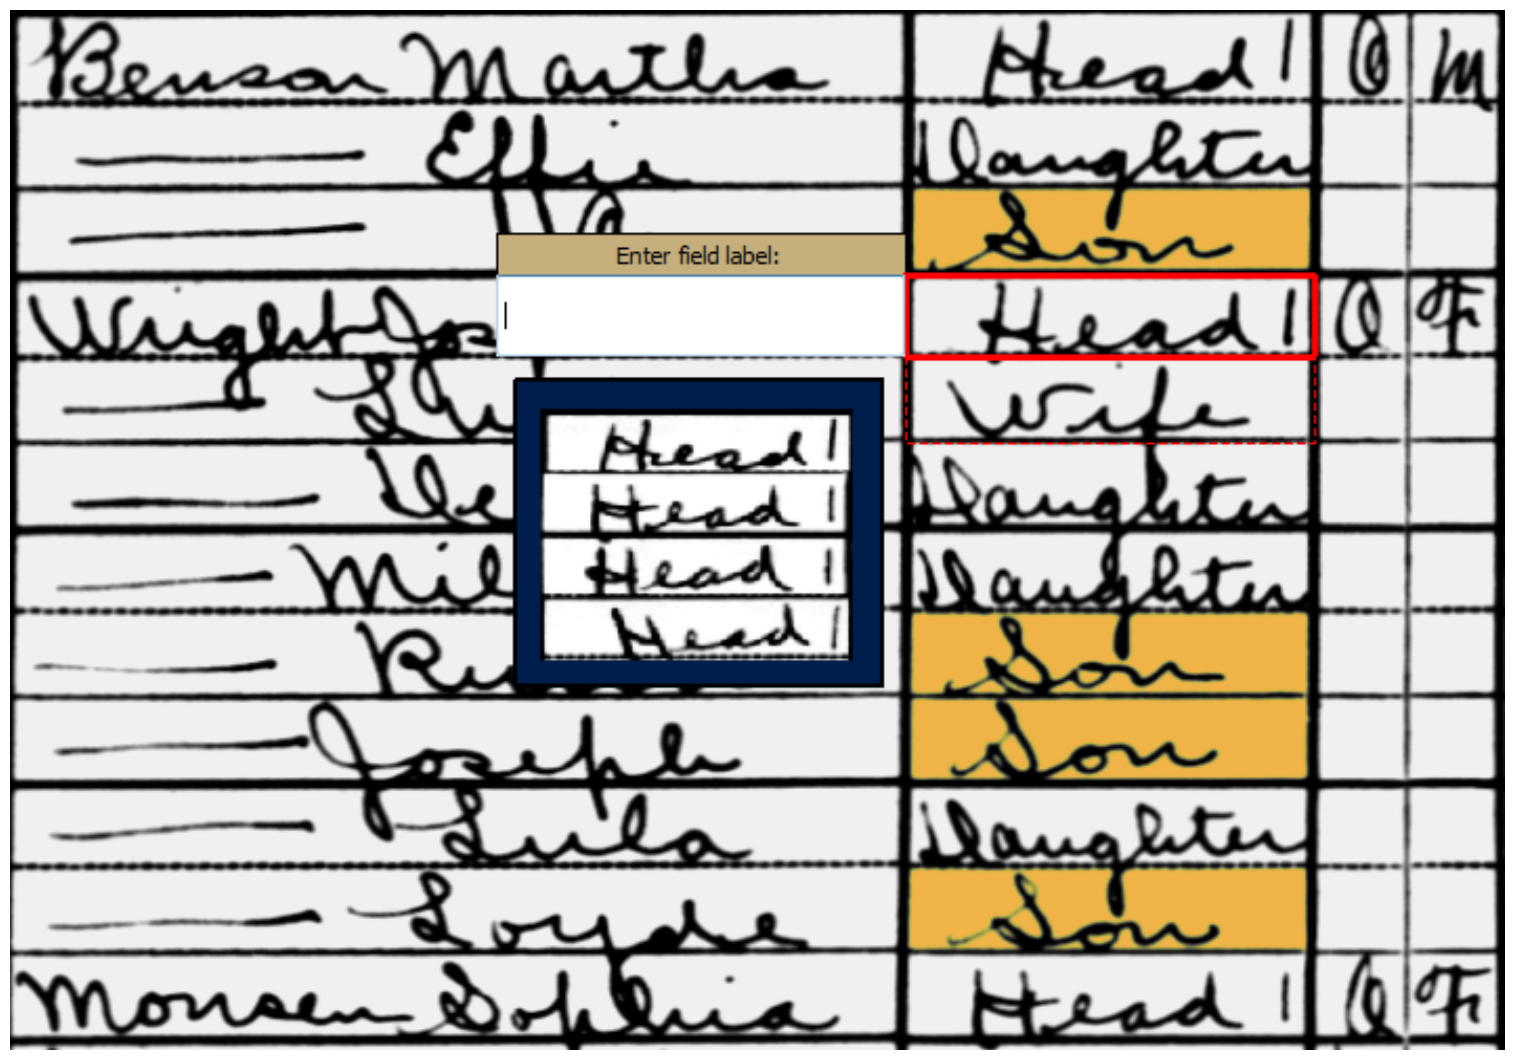
\includegraphics[width=\textwidth]{ii_ex_b}
    		\caption{The matched words,  highlighted in yellow, are all assigned the same user-entered label.}
    	\end{subfigure}
    	\caption{Clawson's CAT system for tabular documents.}
    	\label{fig:ii}
\end{figure}

%"A Framework for Efficient Transcription of Historical Documents Using Keyword Spotting"
Zagoris et al.~\cite{Zagoris2015} \footnote{A demo of their system is found at \url{http://vc.ee.duth.gr/ws/}} presented a CAT system that was also based on word spotting. In their system when the user is transcribing a word image, they are presented with the results of spotting that image (sorted according to rank). The user can then confirm these spottings by clicking on them, causing them to move to a separate list. When this is done, a relevance feedback loop is activated, which submits another word spotting query of the confirmed image. These spotting results are used to refine the ranked list, providing a better selection. Figure \ref{fig:zagoris} shows a screen-shot of their demo system.
%The description of the system is unclear, but we believe the list of confirmed spottings are then labelled the same as the current word image.
We use the same strategy as \cite{Zagoris2015} to guide the combination of our subword spotting results from multiple queries. Further details are given in Section \ref{combine}.

\begin{figure}
    \centering
    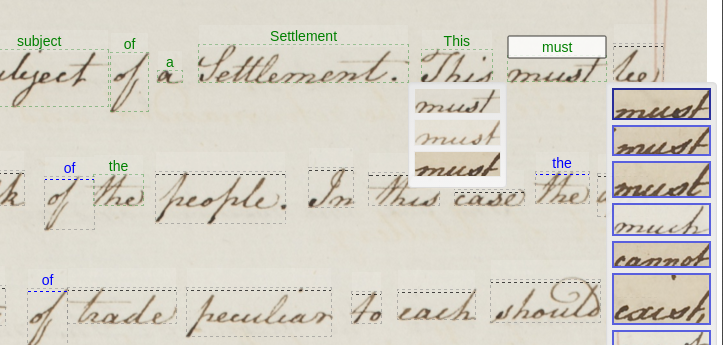
\includegraphics[width=.85\textwidth]{zagoris}
    \caption{A screen-shot of a the CAT system of Zagoris et al.~\cite{Zagoris2015}. The green text indicates hand labeling, the blue text indicates automatic labeling. You can see to the right of the current word (``must'') the current ranked list of spottings (blue boxes).}
    \label{fig:zagoris}
\end{figure}

Neudecker and Tzadok \cite{Neudecker2010} presented a CAT system for historical printed documents that is very similar to the CAT system we present in Chapter \ref{transcription}. The system would first segment the individual characters of the documents and run an OCR engine on them. Those characters with low confidence would then be presented to a user for verification in a character session. A single character session contains all the low-confidence character images classified to a single character. An example of their system's character session for the character ``?'' is given in Fig.~\ref{fig:carpet}.  The user merely needs to select the incorrect classifications. Then in a word session, a word image is shown to the user with possible transcriptions for the word, from which they select the correct one. There are three key strengths of this system. One is that as long as the document’s characters can be segmented, it can work. The second is that it formats all user tasks as selections, rather than typing, and they are quickly completed. This creates a much more enjoyable experience for the user. The third key strength is that it is highly parallelizable for crowd-sourced transcribing. This parallelism is achieved because all character sessions are independent of one another and all word sessions are independent of one another. Our system follows this method's pattern so it has flexibility of document types, simple user tasks and a parallelizable framework.

\begin{figure}
    \centering
    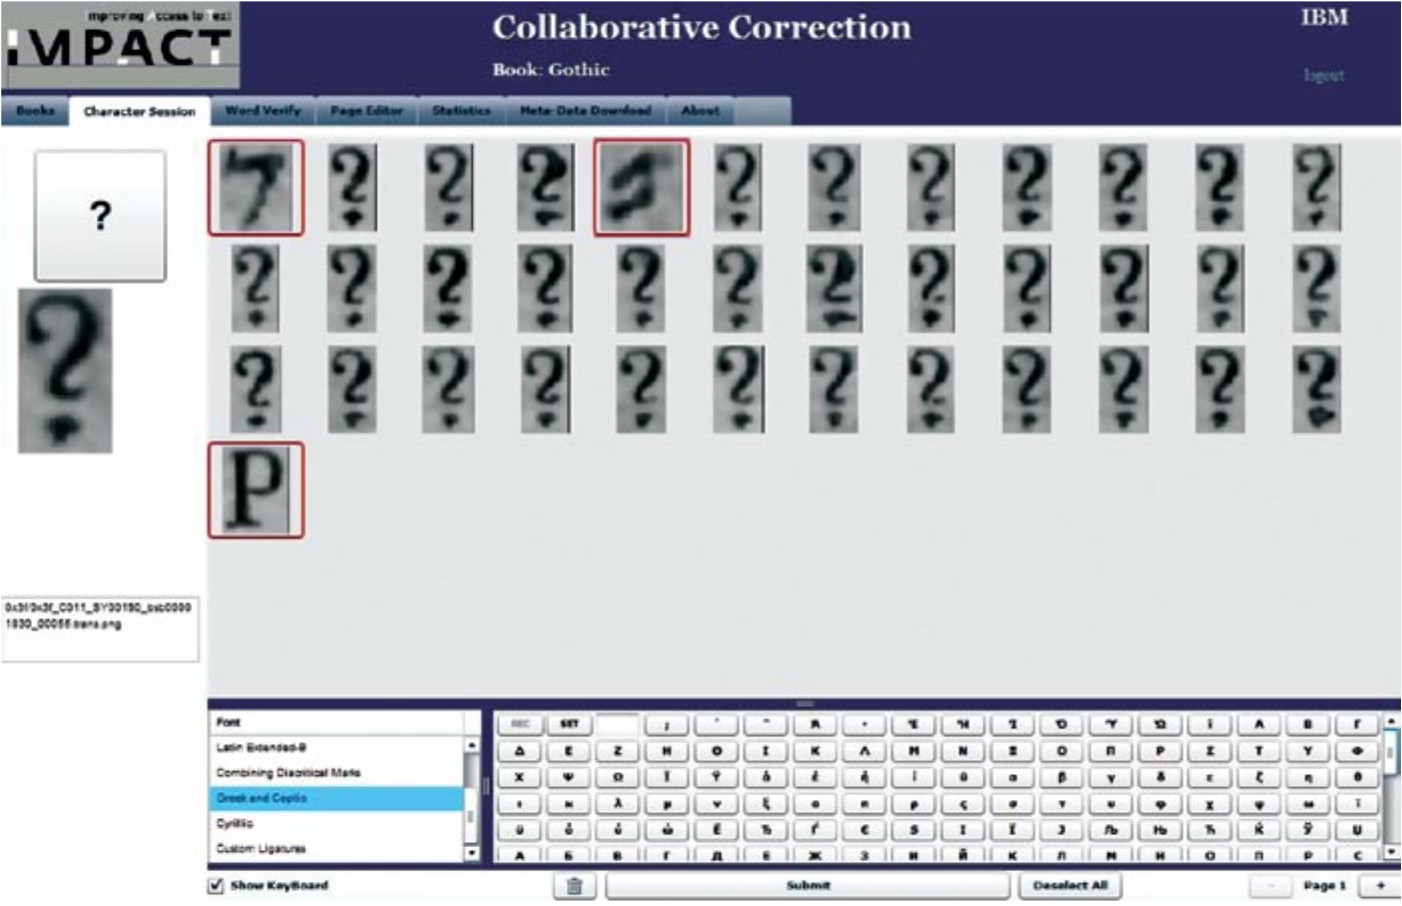
\includegraphics[width=.85\textwidth]{carpet}
    \caption{A screen-shot of a character session for ``?'' from Neudecker and Tzadok's CAT system \cite{Neudecker2010}, taken directly from their report \cite{Neudecker2010}. Notice how easy it is for a user to simply click on the erroneous classifications.}
    \label{fig:carpet}
\end{figure}

Retsinas et al.~\cite{Retsinas2015} expanded on \cite{Neudecker2010} to reduce the amount of user input required by clustering character images together. By viewing an average of a character cluster (where the characters are overlapped), the user can then assign the whole cluster a character label or reject the cluster as being incoherent (i.e.~the cluster contains multiple characters). See Figure \ref{fig:retsinas_ex} for an example. Though requiring more thought from the user, this prevents the tediousness of examining all character images. %Clustering could be applied to our work; it would be more difficult with handwriting, though using online learning to initialize clusters may overcome this. We, however, will not pursue it at this time.
We attempt to use clustering in our own CAT method, however we cannot perform the overlap due to the greater variance in handwriting. Instead we take the approach of \cite{Clawson2014} and simply group clusters together to help visual discrimination.

\begin{figure}
    \centering
    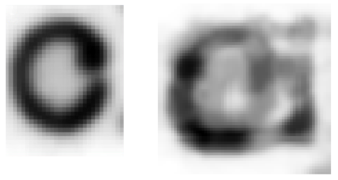
\includegraphics[width=.4\textwidth]{retsinas_ex}
    \caption{Examples of a good cluster (`c') and an incoherent cluster (multiple character classes) taken from \cite{Retsinas2015}.}
    \label{fig:retsinas_ex}
\end{figure}

While we have not seen it done, it would be relatively easy to transfer the results of RNN/CTC-based automatic transcription method to CAT by extracting the top-N transcriptions from the network output. These could then be fed to a user for approval and quick correction for most errors. Given the strength of these automatic methods by themselves, we expect a CAT version of them would outperform the older CAT methods discussed in this section. 



%\section{Other Transcription Assistants}
%TODO

%%%%%%%%%%%%%%%%%%%%%%%%%%%%%%%%%%%%%%%%%%%%%%%%%%%%%%%%%%%%%%%%%%%%%%%%%%%%%%
\chapter{Datasets}\label{datasets}

We use three datasets in our evaluations: the IAM handwriting dataset, the Bentham dataset, and a dataset we extracted from the U.S.~1930 census, which we refer to as Census Names. In this chapter we describe each of these datasets and additionally describe our lexicon.

\section{IAM Dataset}

The IAM handwriting dataset \cite{IAM} is a dataset collected by having human subjects copy certain paragraphs of printed text into handwriting. They were instructed to keep lines well separated and the dataset is very clean as a result. It contains annotations to the word level. We used the provided test set split, the combine training and validation 2 splits as our training set, and the validation 1 set as our validation set.
Example lines from the IAM dataset can be seen in Figure \ref{fig:IAMExamples}.
The test set has 96.1\% of its contents in our lexicon.
These sets have the respective sizes and number of (exclusive) authors:\\
\indent \indent Training: 55106 words, 326 authors\\
\indent \indent Validation: 7089 words, 46 authors\\
\indent \indent Testing: 14600 words, 128 authors

\begin{figure}
    \centering
    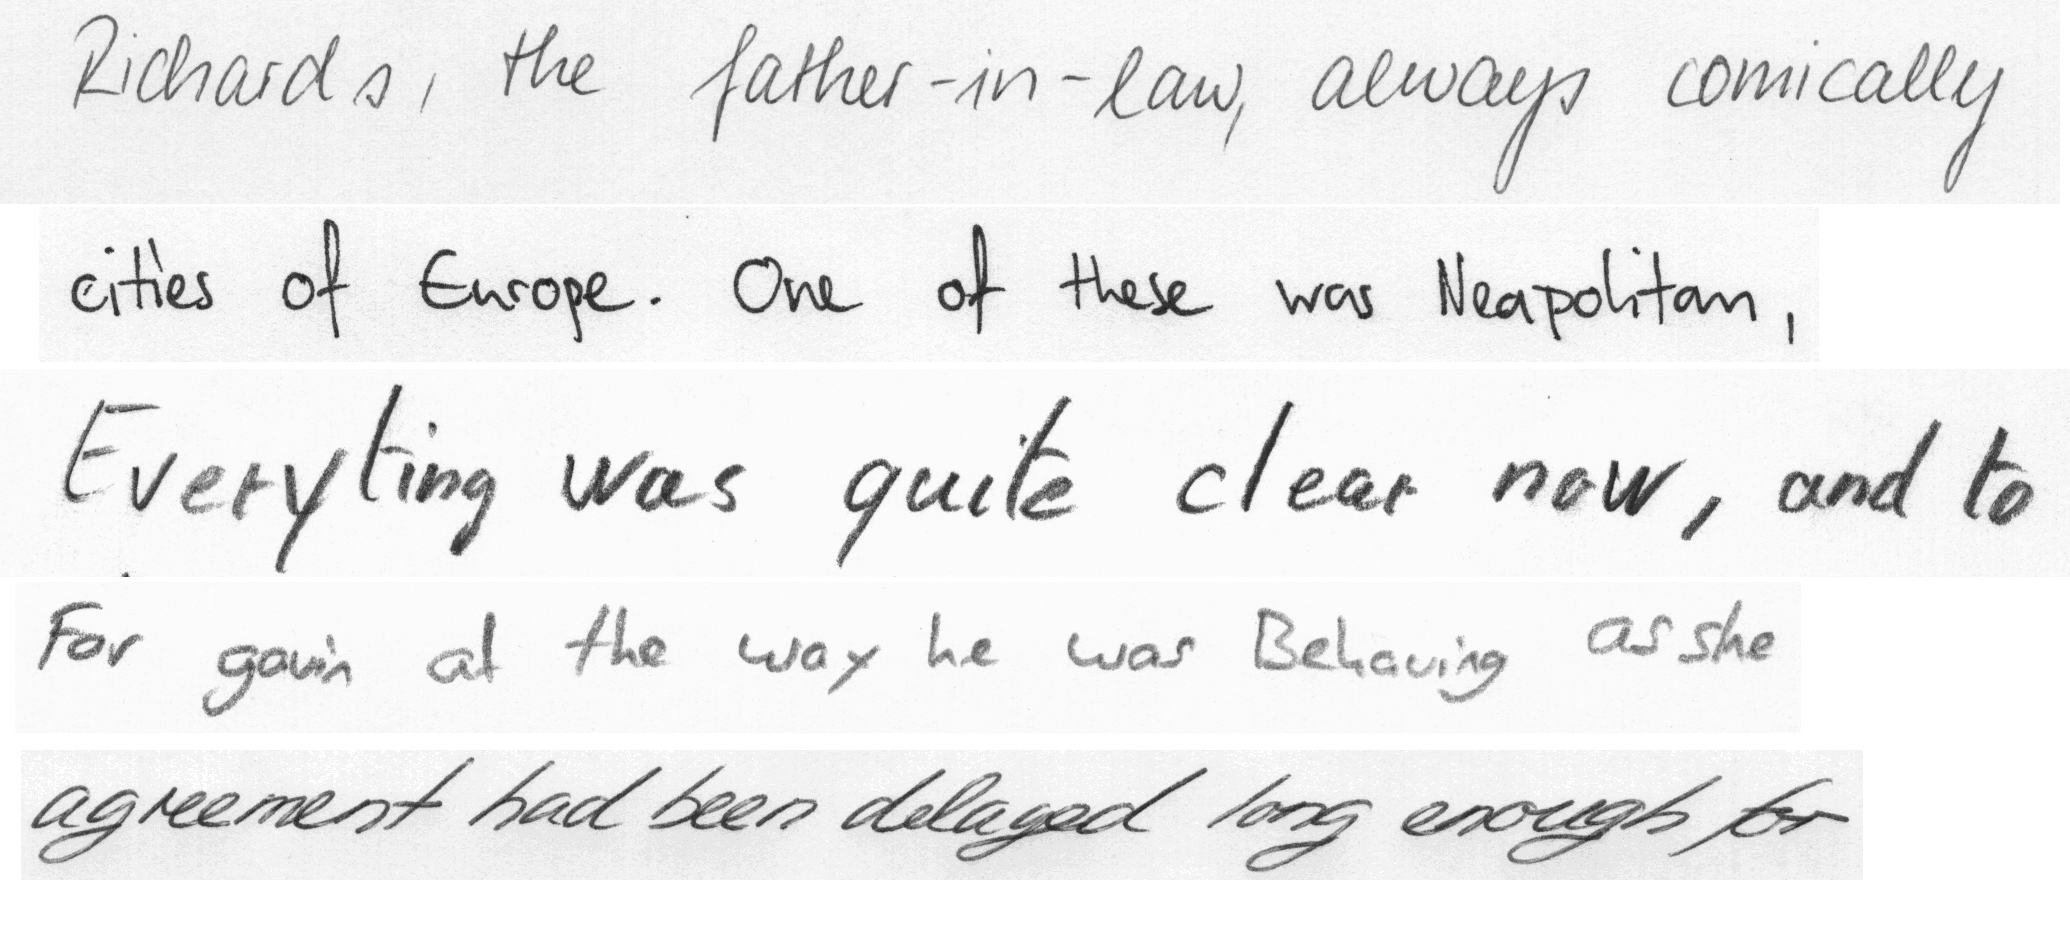
\includegraphics[width=.9\textwidth]{IAM_examples}
    \caption{Examples of lines from the IAM dataset.}
    \label{fig:IAMExamples}
\end{figure}

\section{Bentham Dataset}

The Bentham dataset \cite{bentham} is a collection of documents written by the 17th century philosopher Jeremy Bentham. While there are a plethora of errors we corrected in the ground truth, that ground truth we use differs significantly from that which is officially released, though it is based on it. 
Our training, validation, and test sets are based on the official split, but are not identical.
We ensured pages are exclusive to a single set.
%As we are observing a CAT application of subword spotting it would be optimal that the ``seed'' training set would cover all writing styles. We mix the word instances assigned to the training, validation, and test sets; this likely covers all writing styles and it would be very feasible to randomly label words of a segmented dataset.
Example lines from the Bentham dataset can be seen in Figure \ref{fig:BenthamExamples}.
The test set has 94.9\% of its contents in our lexicon
These sets have the respective sizes:\\
\indent \indent Training: 8490 words\\
\indent \indent Validation: 1071 words\\
\indent \indent Testing: 860 words

\begin{figure}
    \centering
    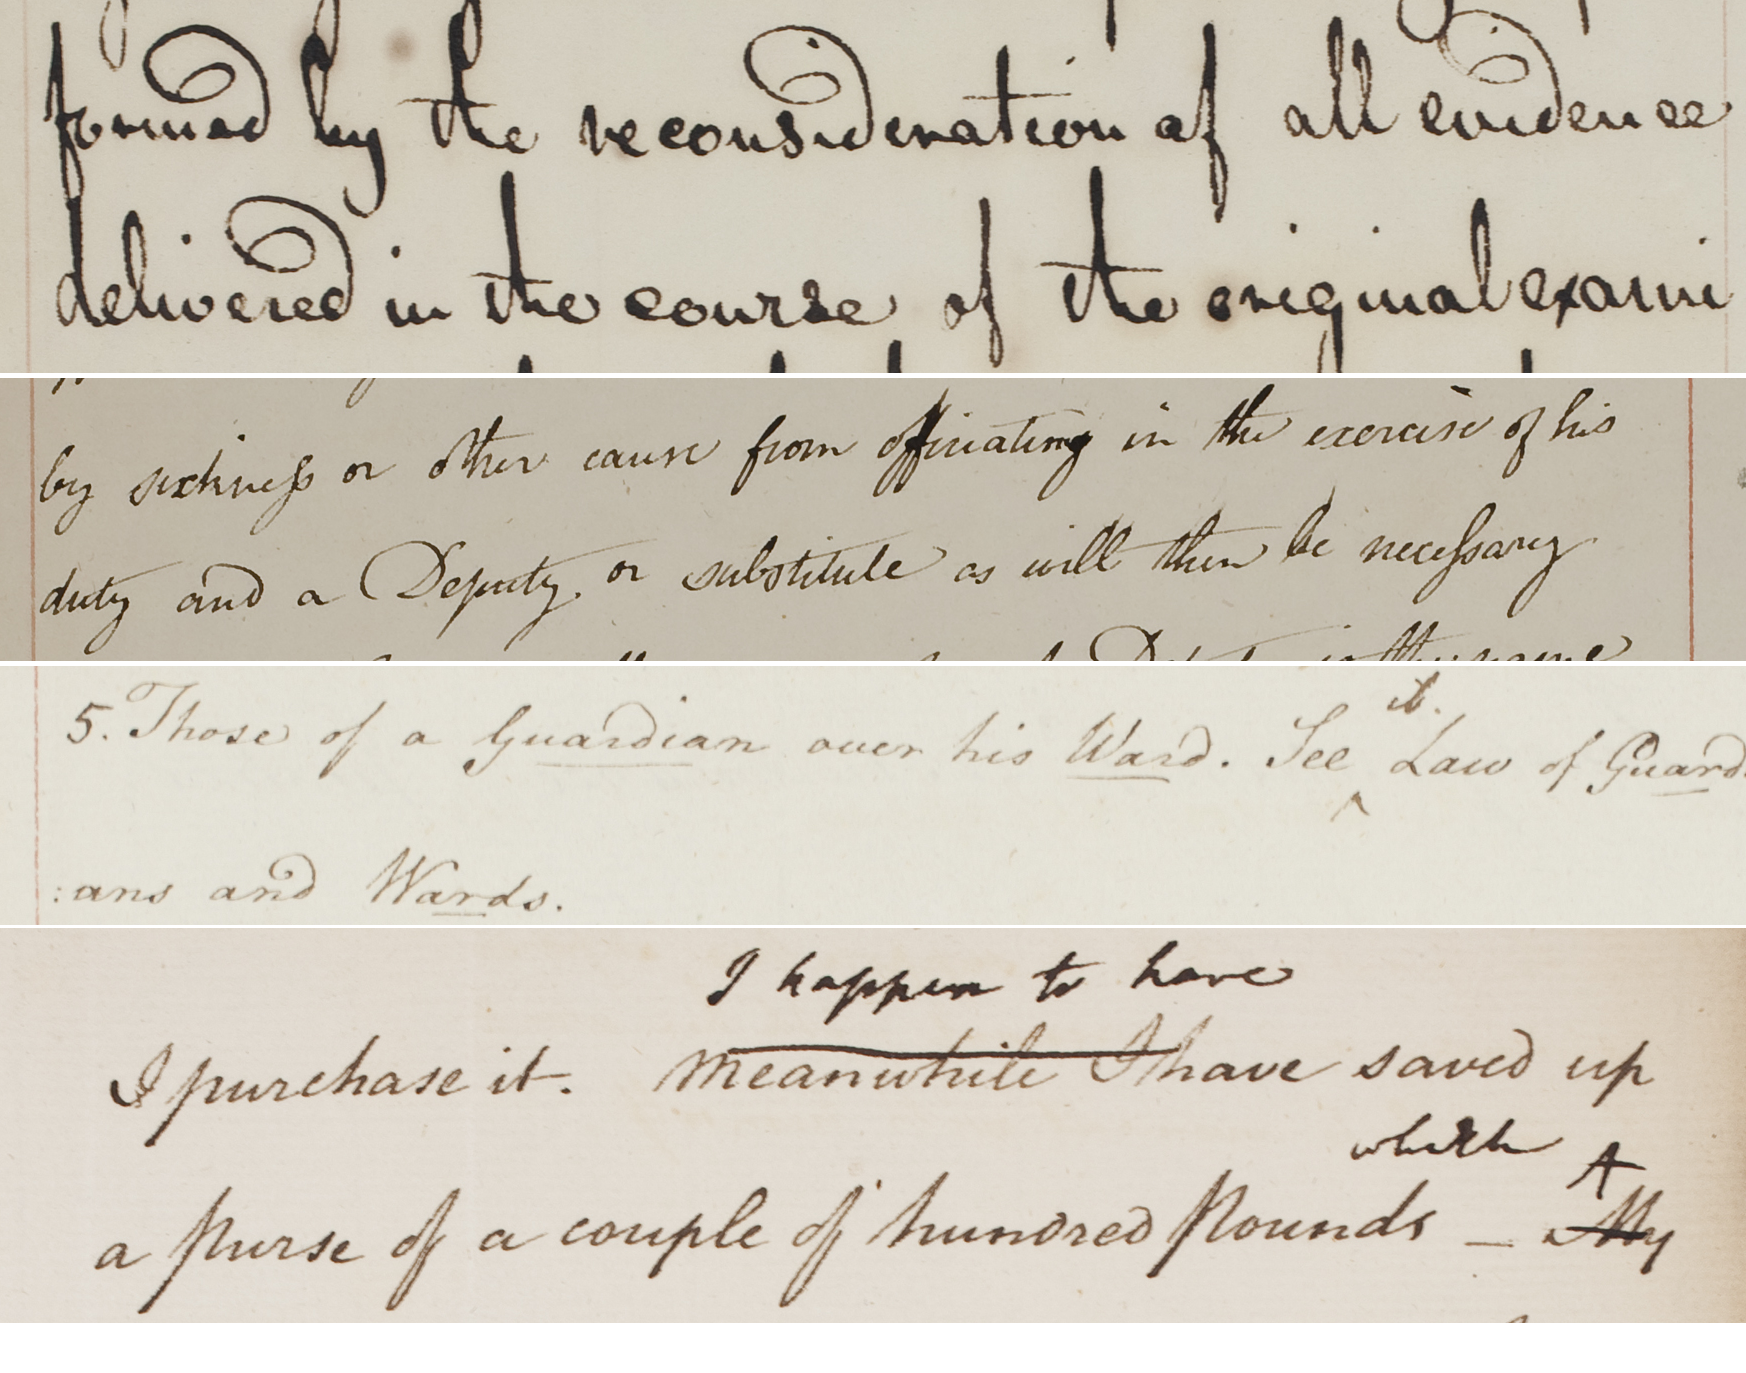
\includegraphics[width=.9\textwidth]{bentham_examples}
    \caption{Excerpts from the Bentham dataset.}
    \label{fig:BenthamExamples}
\end{figure}

\section{Census Names Dataset}

%These files are in py_stuff/census_prep and robert_stuff/document_project/apps_src/field_cropper
The Census Names dataset is an extraction of names from the United Stated of America 1930 census. Example lines from the Census Names dataset can be seen in Figure \ref{fig:NamesExamples}. FamilySearch provided us the ground truth index as well as a  registration of the form images (rotation, scale and offset to align them). We locate the bounding boxes of the name fields by the following process:
\begin{enumerate}
 \item Average the registered images (Figure \ref{fig:makenames} a).
 \item Manually enhance the contrast of the resulting image (Figure \ref{fig:makenames} b). 
 \item Hand annotate the average image with the lines of the form, using straight lines (Figure \ref{fig:makenames} c). 
 \item For each form image peform a more refined registration %individually by doing a second registration with the hand annotated form lines by the following. 
 \begin{enumerate}
  \item Globally move all the form lines together to maximize the summed inverse pixel intensity (darker is better) along the form lines. This is done by scanning 50 pixels in the four cardinal directions separately (Figure \ref{fig:makenames} d). 
  \item Do a more dense scan of all positions in a $7\times 7$ neighborhood around the combined the best x and y positions from the separate horizontal and vertical scans (previous step). %(Figure \ref{fig:makenames} f)
  \item For each individual cell of the form, create a small (12 pixel) vertical or horizontal profile  around each of the four lines forming the cell boundaries (Figure \ref{fig:makenames} e) 
  \item Locally snap each cell wall to the darkest part of it's respective profile (Figure \ref{fig:makenames} f). This yields a very precise registration in most cases. 
  \item Manually segment the words (last name, first name, middle initial/name) within each cell (Figure \ref{fig:makenames} g). 
 \end{enumerate}
\end{enumerate}
The test set has 83.7\% of its contents in our lexicon
These sets have the respective sizes:\\
\indent \indent Training: 6292 words\\
\indent \indent Validation: 718 words\\
\indent \indent Testing: 2130 words


\begin{figure}
    \centering
    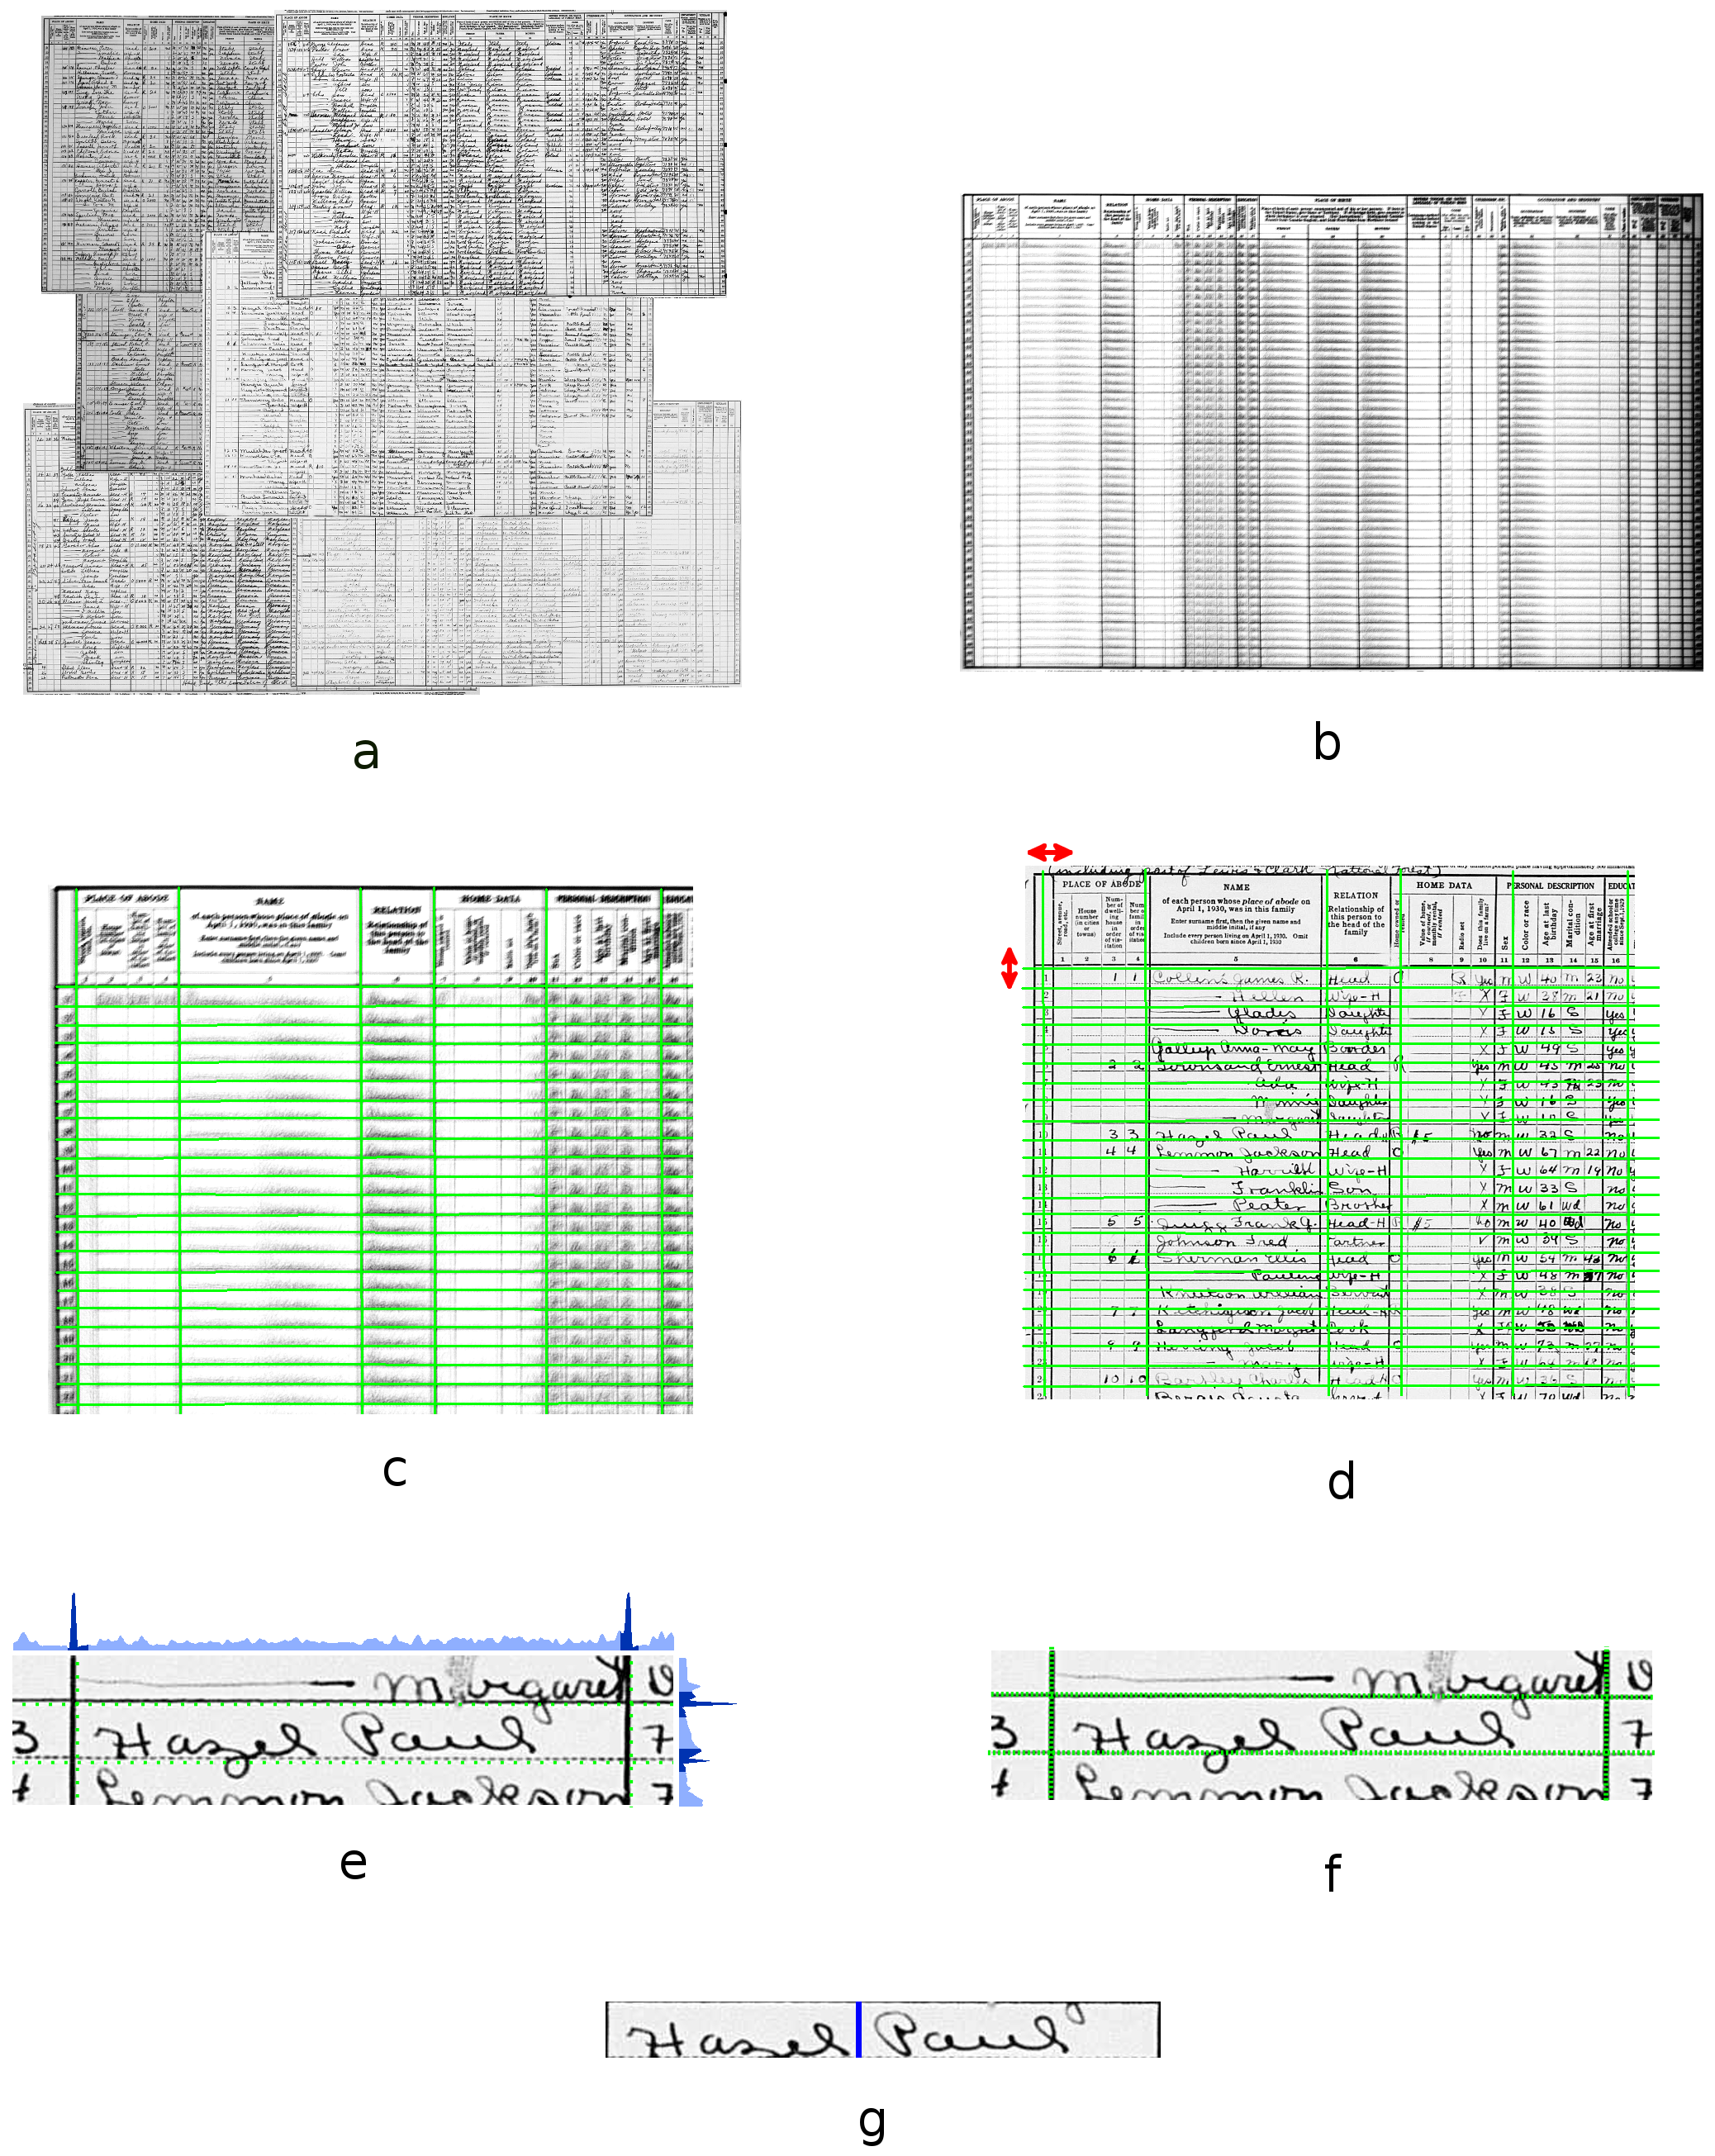
\includegraphics[width=.9\textwidth]{makenames}
    \caption{Process for extracting names from US 1930 census forms for Census Names data set. We begin with registered forms (a). Then we average the images together (b). The average image is used to mark form boundaries manually (c). The lines are registered to specific census image (d). At each cell a peojection profile is computed around the cell boundaries (dark blue) (e). The cell boundaries are snapped to the histogram peaks (f). Word boundaries were manually annotated for each cell (g).}
    \label{fig:makenames}
\end{figure}

\begin{figure}
    \centering
    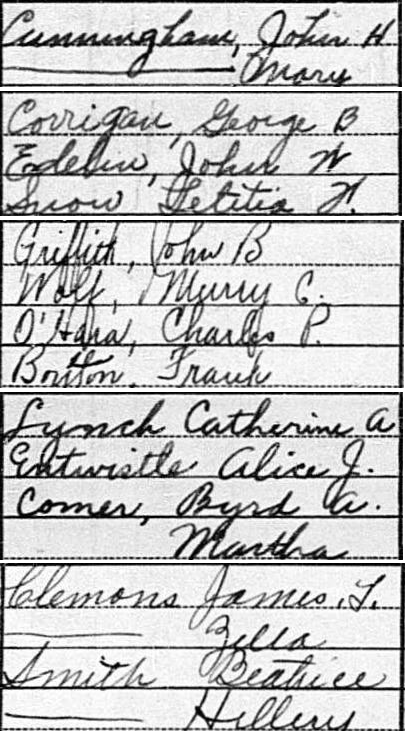
\includegraphics[width=.5\textwidth]{names_examples}
    \caption{Excerpts from the Census Names dataset.}
    \label{fig:NamesExamples}
\end{figure}

\section{Character Annotation}

For the testing portion and a small validation set of the Bentham and Census Names datasets, we produced a character segmentation ground truth. We annotated the word segmentation ground truth by marking the point between characters, meaning character boundaries do not overlap, in addition to a tighter start and end boundary for the word (first and last letters), as seen in Figure \ref{fig:charseg}.

\begin{figure}
    \centering
    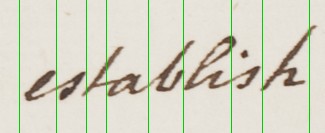
\includegraphics[width=.5\textwidth]{charseg}
    \caption{Example of hand annotated character segmentation.}
    \label{fig:charseg}
\end{figure}

\section{Lexicon}

%Lexicon was created with extractMostFrequentNames.perl
%Merged(intersection) wordsEn.txt with last and first names with 1000 frequency count.
%108,028 words and 6,939 names
%SIL International, linguistics site
For our CAT (computer assisted transcription) methods, we require a lexicon. We choose to use a large English lexicon as this would indicate the methods could generalize to other corpi. We obtained a lexicon from SIL International at \url{http://www-01.sil.org/linguistics/wordlists/english/} which contained 108,028 words (not including names). We also desired a large lexicon of names which would enable the Census Names dataset to be transcribed. FamilySearch provided us with data from the US 1940 census, which listed all names appearing in those records along with a count of how many times they occurred. We took all names occuring at least 1000 times, leaving us with a list of 6,939 unique names. Combining these two sets gave us a lexicon size of 114,968. We use the full lexicon for the Bentham dataset, but only the names portion for the Census Names dataset.

%%%%%%%%%%%%%%%%%%%%%%%%%%%%%%%%%%%%%%%%%%%%%%%%%%%%%%%%%%%%%%%%%%%%%%%%%%%%%%
\chapter{Subword Spotting}\label{subwordspotting}
%""
%We implemented multiple CAT systems to provide a well rounded view of transcription through subword spotting. In this chapter we first describe our (sub)word spotting method, then the three CAT systems: transcription through PHOC vectors, transcription through approved subword spottings, and transcription through unassisted subword spotting.

Subword spotting is an extension of traditional word spotting where we allow instances to occur within words. We attempt to localize the spotting in the word to provide spatial information. In this work, we focus on small subwords as most applications of subword spotting we explore in Chapters \ref{applications} and \ref{transcription} use these. Figure \ref{fig:explain_sub_spotting} shows an example subword spotting.

In this chapter we describe our implementation of subword spotting and then evaluate many aspects of its performance, including full word, uni-, bi-, and trigram spotting as well as multi-query aggregation.


\section{Implementation}

We use a sliding window over word images with a word spotting CNN to perform subword spotting.

\subsection{Architecture}

Our subword spotting is built on the segmentation based word spotting method PHOCNet \cite{sudholt2016, sudholt2017} which we adapted to perform a sliding window over the word images. \cite{sudholt2017} uses a deep convolutional network trained on word images with pyramidal histogram of characters (PHOC) \cite{Almazan2014} as the target vectors. This method can word spot using both query-by-string (QbS) and query-by-example (QbE), that is a query may be a text word or a word image. Searches are performed simply by comparing vector similarities, the query vector either being a word's PHOC vector if searching with text or found from running its image throught the network. See Section \ref{relatedwork_wordspotting} for the details of PHOC vectors. We follow \cite{sudholt2017} and use a PHOC vector where the alphabet is case insensitive, includes digits (0-9) and does not include bigrams (unlike \cite{Almazan2014} which uses bigrams in the first two layers). For our specific application of subword spotting, we try adapting the PHOC vector in \cite{sudholt2017} so instead of having levels 2,3,4,5 we have 1,2,3. \cite{sudholt2017} was designed for words which require more spatial resolution than subwords. Our PHOC levels directly correspond with the fact we are spotting uni-, bi- and trigrams. We refer to this as our ``adapted PHOC'' in the results.



Our network architecture varies slightly from \cite{sudholt2017} and is outlined in Figure \ref{fig:network}. We note the reduction in the number of channels in the layer before the temporal pyramid pooling (TPP) and fully connected layers (from 512 to 128); this is to reduce the size of featurized images (which are saved after this layer).  We used Sudholts's code available on GitHub (\url{https://github.com/ssudholt/phocnet}), which uses the Caffe framework \cite{caffe}.

%SPP \cite{SPP} is a method of allowing a network with fully connected layers to handle images of arbitrary size. This is accomplished by performing a pooling (max in our implementation) over windows of the image. The first window encompasses the full image and then it proceeds by dividing the windows into 4 at each level down. We use 3 levels for all datasets except the Census Names dataset, which has smaller characters. We use 2 levels for the Census Names dataset to allow the network to operate on smaller images (the SPP won't be creating windows of subpixel size).

TPP is a slight modification of spatial pyramid pooling (SPP) \cite{SPP}, which is a method of allowing a network with fully connected layers to handle images of arbitrary size. This is accomplished by performing a pooling (max in our implementation) over windows of the feature map (image). The first level is a window that encompasses the full image. The second level is four windows dividing the image into fourths (each the size of half the image width and half the image height). The proceeding levels follow a simlar pattern. TPP uses the same idea, but only divides windows horizontally as verticle information is not useful once word images are featurized. We use 5 layers (dividing the image into 1, 2, 3, 4, and 5 even windows). Figure \ref{fig:TPP_example} shows what TPP looks like visually. %for all datasets except the Census Names dataset, which has smaller characters. We use 4 layers for the Census Names dataset to allow the network to operate on smaller images. 
We modify TPP slightly to handle the corner case of small images such that the windows are adjusted to be slightly overlapping at a particular level if a window had a width of zero at that level.

%TODO image for TPP

\begin{figure}[t]
    \centering
    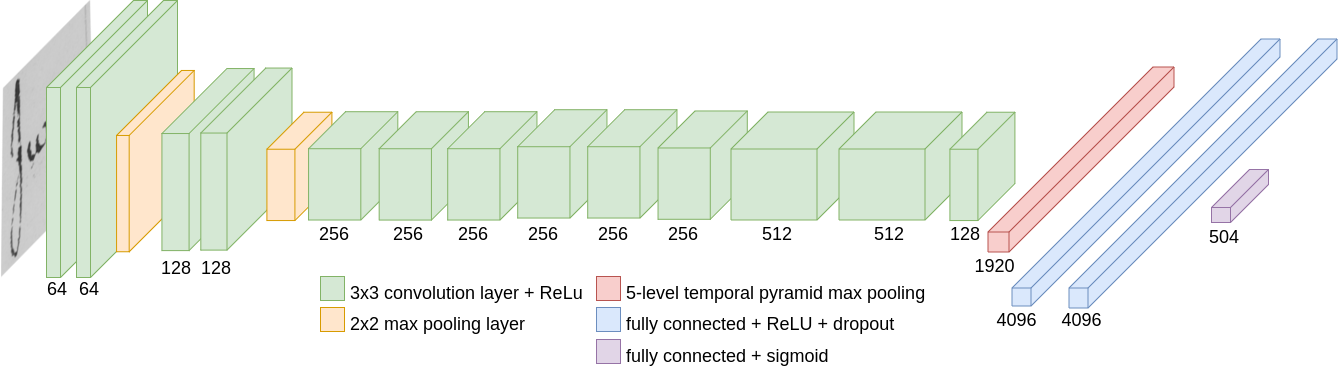
\includegraphics[width=.98\textwidth]{thesis-phocnet}
    \caption{Network architecture for embedding images as PHOC vectors. The numbers beneath each layer represent the number of channels. As the network uses temporal pyramid pooling before the fully connected layers, it can accept images of any size. Our architecture differs from \cite{sudholt2017} only in the number of channels of the last convolutional layer.}
    \label{fig:network}
\end{figure}

\begin{figure}[t]
    \centering
    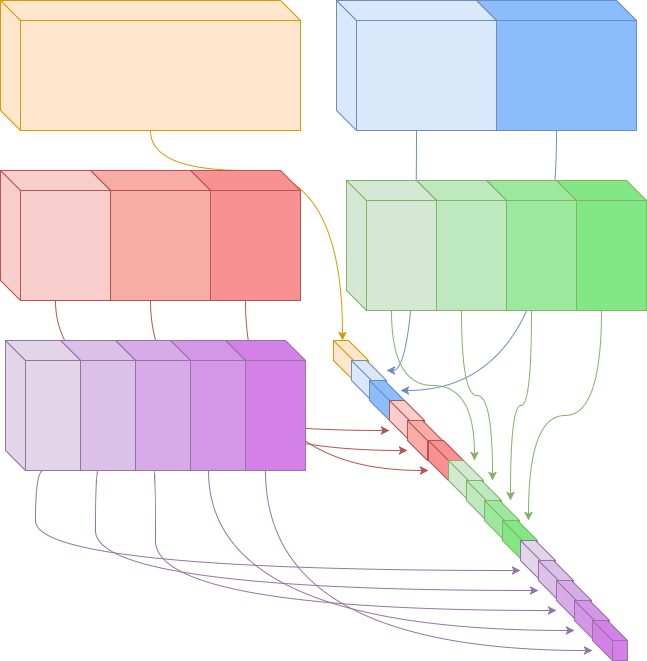
\includegraphics[width=.55\textwidth]{TPP_example}
    \caption{What temporal pyramid pooling (TPP) looks like visually. The same network features (large blocks) is divided into even horizontal windows of different counts (1,2,3,4,5 here). The result of pooling each of these windows (max pooling in our implementation) is appended together as an output vector. This is the red vector in Figure \ref{fig:network}.}
    \label{fig:TPP_example}
\end{figure}

\subsection{Training}

In training, we used a batch size of 10, a learning rate of $10^{-4}$, weight decay of 0.00005, and the Adam optimizer \cite{adam}.
%decay the learning rate so that the learning rate at iteration $i$ is $r_i = r_0 (1 + 0.0001 i)^{-0.75}$ (``inv'' policy in Caffe).
%We train until out validation loss begins to increase (passes a minimum), indicating overfit, or flatlines for a significant number of iterations.
%We then test the validation set MAP for various iterations to find the maximum performance, as MAP generally peaks differently than the loss.
We train the model out 240,000 iterations, droping the learning rate by a factor of 10 for the last 10,000 iterations. We note that the model does not appear to overfit at this point, but gains at this point in training are minimal.
%The final iterations for our trained models are as follows. IAM:X, Bentham:X, Census Names:X.
%We then begin training with a learning rate of $10^{-5}$ 4000 iterations prior to the MAP peak, stopping again when the validation loss begins to increase. 
%We then repeat the process of finding the validation MAP peak.

We use the same data augmentation as \cite{sudholt2017}, which consists of balancing the training set according to word occurances (by their text) and distorting duplicate instances with random affine transformations.

%During training, we use a distortion augmentation technique similar to the one described in \cite{wigington2017}. In the augmentation technique each example is distorted by placing control points in grid fashion on the image and then distorting the image by perturbing these control points. This is repeated at finer scales; the control points are more closely aligned and the perturbations smaller. See Figure \ref{fig:augmentation} to see the result of this augmentation on a word image. This augmentation greatly reduces possible overfitting during training as the network never sees the exact same images twice.
%For the Bentham dataset we started with control points $d_0 = 64$ pixels apart and initial perturbations with a standard deviation of $\sigma_0 = 0.3 d_0$. We decreased control point distance by a factor of 0.5 and decreased the perturbation standard deviation by a factor of 0.6 for each of 4 levels, so that if $l$ is the level, $d_l = 64(0.5^{l})$ and $\sigma_l = 0.3 d_l (0.6^{l})$.

%Similar to \cite{sudholt2016} we balance word counts in the training set. However, we allow far more instances of each word (more duplicates of images) in the training set due to our improved augmentation technique. We set a goal for the count of each word of $c_{goal} = 0.6c_{max}+0.4c_{mean}$, where $c_{max}$ is the maximum count of any word and $c_{mean}$ is the mean count of all words ($c_{max}$ is capped at 150 to prevent too large of training sets). A set of $c_{goal}$ instances of each word form the training set, including some duplicates when needed. Also following \cite{sudholt2016}, duplicate images in the dataset have a random affine transformation applied to them. We differ slightly from the implementation \cite{sudholt2016} used, as they did not resize images to capture pixels moved off of the origin images frame by the transformation; we do this as we find it slightly enhances performance.

%Each word image is a unique size, however, to train on a GPU all instances in a batch must be the same size. We circumvent this by resizing all word images in a batch to the same size. The height and width composing this size are drawn from Gaussian distributions parametrized by the mean of the height and width of
%the word images of the batch, the standard deviations being $2/3$ the standard deviation of the height and width of the batch images. This is additionally capped at a maximum and minimum height (120,1) and width (600,20). This process slows training, as the network must be resized every iteration. To minimize this, it a new batch size is within a threshold (height 15 pixels, width 20 pixels) of the previous batch size, the previous batch size is used. While the network sees slightly less variation is size, it significantly speeds up training.

%We used a validation set to determine the optimal number of training iterations by observing when QbS word spotting on the validations set peaked in performance.

%NOT TRUE ANY MORE? not in training at least
%To prevent images too small for the network (SPP layer is sensitive to this), any instances smaller than 32 pixels in their smallest dimension are resampled with a larger bounding box. Additionally 
%We scale any images taller than 200 pixels to be 200 pixels tall; this improves efficiency and provides some normalization to the titles found in the Bentham dataset.

%\begin{figure}
%    \centering
%    \begin{subfigure}[t]{0.46\textwidth}
%    		\centering
%    		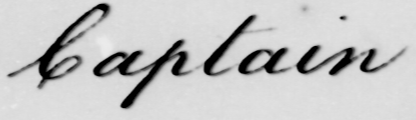
\includegraphics[width=\textwidth]{Captain_unwarped}
%    		\caption{Unwarped image.}
%    	\end{subfigure}
%    	~
%    	\begin{subfigure}[t]{0.46\textwidth}
%    		\centering
%    		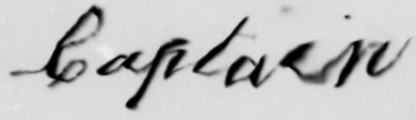
\includegraphics[width=\textwidth]{Captain_warped}
%    		\caption{Image warped using augmentation technique from \cite{wigington2017}.}
%    	\end{subfigure}
%    	\caption{Example of data augmentation used in training.}
%    	\label{fig:augmentation}
%\end{figure}

\subsection{Determining Window Widths}\label{detirminewindowsize}
Because the neural network takes in some context, it is difficult to measure what the optimal sliding window size should be, based on visual width.
Additionally each n-gram is likely to have a different optimal window size. We determine the optimal window size for each n-gram as follows.
We first compute the MAP for a range of window sizes (stepping 4 pixels), smoothing these results and taking the max. We smooth by averaging a window of 3 steps (average MAP from 3 window sizes), using 2 steps on the edges. For efficiency we cluster all the resulting window sizes (from each n-gram) into 10 clusters using k-means, assigning each n-gram the cluster mean as its width. This allows us to pre-compute PHOC vectors of only 10 window sizes.% for all n-gram.

We note that refining the window size during spotting to maximize the score for a specific word image does not give improvements overall.

Our optimal sizes are reported in the Appendix in Table \ref{tab:customwidths}.

%We report the optimal widths we found in \ref{appendiX} %TODO

\subsection{Running}

To prepare for spotting, we save the output of the network before the TPP layer as a featurization of each word image. Then subwindows of this featurization can be passed to the latter part of the network (starting with TPP) to generate a PHOC vector. As part of the preprocessing we extract PHOC vectors for subwindows with a stride of 4 pixels (step of 1 in the featurized image as the network reduces images by a factor of 4) for the 10 sizes determined using the method in the previous section.

%the number of characters being spotted and an estimated character width for the dataset; 37? 33 pixels for the Bentham dataset, 20 for the Census Names dataset.
%This preprocessing allows us to forgo running the network as we merely need

%For performing QbS, one compares the PHOC vector representing the query word or n-gram to the output of the network. For QbE, the outputs of the network are compared against eachother.
\cite{sudholt2017} uses a cosine similarity to compare PHOC vectors (both string and network generated). We used this, but also tested other comparison methods and found that for string generated PHOC vectors, using cross-entropy performs better. This is what the network is optimizing and as the training labels are string generated PHOC vectors it makes sense this should perform well. The query vectors for network generated vectors (QbE queries) are noisy and appear very different. We also found improvements by masking out irrelevant levels of the PHOC for the given n-gram being spotted. For unigram spotting we only use level 1, for bigrams levels 1,2 and for trigrams levels 1,3. This masked-cross-entropy comparison is the measure we use for QbS and we use cosine similarity for QbE.
% We note that \cite{sudholt2016} (the original PHOCNet) uses the Bray-Curtis similarity, which yields inferior results with our implementation. We believe the change from SPP to TPP is the reason.
%, however, we found a dot-product similarity, normalizing network outputs, worked better for our implementation.
%The score for a subwindow is the normalized dot product between the query PHOC vector (the network output of the query image or the actual PHOC vector of the query word) and the network's generated PHOC vector for that subwindow.
%To reduce computation, we only return the top two highest scored subwindows of a word image which are at least 40\% of the window size apart. Here, we assume an n-gram never occurs more than twice in a word.%, which is a reasonable assumption for English.


%We tried refining top scoring subwindows by slightly adjusting their boundaries and re-scoring, however, we did not see a significant improvement. %and the computation cost was prohibitive (as the featurization of the refined subwindows was not precomputed).

\subsection{Combining QbE Results}\label{combine}

In one of our tests, we perform aggregation of QbE results by merging results from different queries. To do this we check for potential overlapping spottings between two sets of results, where overlap is defined as when the predicted bounding boxes overlap by at least 20\%. If there is an overlap we discard the result with the worse score. This can be trivially be repeated for multiple queries as we essentailly are finding the max score. Merging by taking the better score follows what \cite{Zagoris2015} found to be most effective when combining full word spotting results. As further justification, one can think of each n-gram or word as having several prototypical ways it can appear (e.g.~an `a' appearing with or without the tail on top, `\textsf{a}' or `{\fontfamily{qag}\selectfont\footnotesize a}'). By selecting the best score you select the score computed on the exemplar image with the prototype closest to the instance of interest's prototype.

%In the following section we show results of this network's performance on unigrams, bigrams, trigrams and whole words.

%%%%

\section{Analysis of Subword Spotting}

In this section we present results of testing the subword spotting method described above.
%We present our own results of testing the subword spotting method described in Chapter \ref{subwordspotting}. 
As a baseline, we show our network's performance on full word spotting. We evaluate subword spotting of unigrams, bigrams and trigrams against our testing portions of the Bentham dataset and Census Names dataset. 

\subsection{Full Word Spotting}

Full word spotting is performed as described in \cite{sudholt2016}, where the neural network is used to generate a PHOC vector of each word image in the corpus. For QbS, each word (string) in the corpus's PHOC representation is used as a query. For QbE, each image which has at least one of image with the same label is used as a query. We compare using mean average precision (MAP). Our results are shown in Table \ref{tab:wordspottingresults} for the Bentham dataset, the Census Names dataset, and, for comparison with PHOCNet \cite{sudholt2016,sudholt2017}, the IAM dataset.

\begin{table}
\centering
\begin{tabular}{| l | c  c | c c | c c |}
  \hline
   & \multicolumn{2}{c|}{IAM} & \multicolumn{2}{c|}{Bentham} & \multicolumn{2}{c|}{Census Names}\\
  Method & QbS & QbE & QbS & QbE & QbS & QbE\\
  \hline		
  %Old network & 0.755 & 0.683 & 0.762 & 0.811 & 0.525 & 0.511  %results with msfNoLRN/sig-bray IAM:208000  BEN:160000 NAMES(less):144000
  Our network  &  0.892 & 0.833  &  0.926 & 0.971  &  0.758 & 0.858  \\%results with phocnetSkinny(Adam,dot) IAM:124000  BEN:X NAMES(less):124000
  Our network adapted PHOC  &  0.868 & 0.809  &  0.935 & 0.975  &  0.755 & 0.864 \\
  %bentham:ben_fixed_corpus.gtp
  
  PHOCNet\cite{sudholt2016} & 0.830 & 0.725 & - & - & - & - \\
  TPP-PHOCNet\cite{sudholt2017} & 0.934 & 0.827 & - & - & - & - \\
  %? & X & X & X & X \\
  \hline  
\end{tabular}
\caption{MAP for full word spotting results, reported for both query-by-string (QbS) and query-by-example (QbE).}
\label{tab:wordspottingresults}
\end{table}

%We first note that our model significantly under performs \cite{sudholt2016} on the IAM dataset (by 7.5\% on QbS and 4.2\% on QbE). We were unable to reproduce their results, mimicking their model, and the architecture changes we make we expected would have a negative effect on performance. It is likely a better word spotting model could be produced, but this was not the the focus of our work.
%It is clear that the Census Names dataset is significantly more challenging than the other datasets, however, having above 50\% MAP indicates the network is learning the task to some degree.
It can be seen that we underperform compared to \cite{sudholt2017}. This is to be expected as we have reduced the number of parameters in the  	CNN model. The adapted PHOC vector performs variably against compared to the original,  performing better in some cases which is suprising as we have reduced its descriptive power for words longer than three characters. It may be the reduced description was easier for our reduced network to learn.
%The adapted PHOC vector performs even worse which is also anticipated as we are reducing its descriptive power for words longer than three characters.

As a note, it is not always meaningful to compare QbS scores to QbE scores, as QbS represents a mean over text queries, one for each possible word label and QbE represents a mean over instance queries, one for each instance of a word in the dataset, meaning it is biased towards the performance of common words (or n-grams in later tests).

\subsection{Subword Spotting}

We use our sliding window method to evaluate spotting uni-, bi- and trigrams. We used our ground truth for the testing portion of the Bentham and Census Names datasets which have character boundaries. We considered a spotting to be correct if its window overlapped with the desired n-gram's boundaries by 0.5 of the smallest of the two's boundaries.
%In the case of multiple spottings with over 0.5 overlap, we discard the spotting with the lesser overlap so as to not count a two true spottings for the same instance.
We spotted each letter of the alphabet, the 100 most frequent bigrams (in the English language), and the 300 most frequent trigrams. Each of these n-grams were spotted using QbS, if there was at least one instance of it in the testing set. All examples of these n-grams in the dataset were used as a QbE query, if there are at least two instances of the n-gram in the test set.

Owing to the fact that a single word may have multiple instances of an n-gram we align the spotting results to their nearest instance. If multiple spottings claim the same instance and are both overlapping enough to be considered a positive match, we only keep the one overlapping the most.
If an n-gram instance is not claimed by any spotting, we add a psuedo result that with the maximum spotting score to the MAP calculations to ensure it properly reflects the missed n-gram.

Results can be seen in Table \ref{tab:subwordspotting}.
Some qualitative results are show in Figures \ref{fig:qualSpot} and \ref{fig:qualSpotNames} for the Bentham and Census Names datasets respectively.
%We show QbS results for both using all n-grams (full) and those n-grams used for QbE (same).


%Trigrams, having the most context, perform the best by a wide margin. Bigrams and unigrams have very comparable performance. Consistently QbS outperforms QbE, we expect this is because the learned representations of the n-grams (used in QbS) are more invariant than individual n-gram instances, which can have large variation in their context and form.

%fawkes...BENTAN/outUni [Bi,Tri] has top 15 spottings

\begin{table}
\centering
\begin{tabular}{| r | c c | c c |}
  \hline
   %& \multicolumn{2}{c|}{Bentham} & \multicolumn{2}{c|}{Census Names}\\
   %& QbS & QbE & QbS & QbE \\
   & \multicolumn{2}{c|}{Bentham} & \multicolumn{2}{c|}{Census Names}\\
   %&     & weighted & n-gram & instance &     & weighted & n-gram & instance \\
   & QbS  & QbE    &  QbS &  QbE    \\
  \hline 
  Original PHOC using cosine similarity & & & & \\
  %cosine similarity
  Unigram &  0.654 &  0.511  & 0.480 &  0.340 \\
  Bigram  &  0.549 &  0.569  & 0.375 &  0.294 \\
  Trigram &  0.522 &  0.571  & 0.271 &  0.285 \\
  \hline
  
  Adapted PHOC using cross entropy & & & & \\
  %net-adapted + masked cross ent   old ww
  Unigram &  0.677 &  0.327  & 0.497 &  0.203 \\ 
  Bigram  &  0.682 &  0.426  & 0.402 &  0.179 \\
  Trigram &  0.705 &  0.441  & 0.363 &  0.170 \\
  \hline 
\end{tabular}
\caption{MAP for subword spotting results on the Bentham and Census Names datasets, reported for query-by-string (QbS) and, query-by-example (QbE).}
\label{tab:subwordspotting}
\end{table}

\begin{table}
\centering
\begin{tabular}{| l | c c c | c c c c |}
  \hline
   & \multicolumn{3}{c|}{PHOC \cite{sudholt2017}} & \multicolumn{4}{c|}{Adapted PHOC}\\
   %&     & weighted & n-gram & instance &     & weighted & n-gram & instance \\
   & Cosine & CE & Masked CE & Cosine & CE & Masked cosine & Masked CE   \\
  \hline   
  \hline 
  QbS & & & & & & & \\
  \hline
%                                                                         redo CE, final final2(uni, no mask)
%Unigram &  0.654 &  0.608 &  0.654 &  0.678 &  0.691 &  0.499 &  0.691 \\,0.677  0.570, 0.677,
%Bigram  &  0.549 &  0.641 &  0.679 &  0.643 &  0.665 &  0.571 &  0.665 \\,0.682  0.663, 0.663,
%Trigram &  0.522 &  0.560 &  0.612 &  0.618 &  0.640 &  0.586 &  0.659 \\,0.705  0.697, 0.697,
Unigram &  0.654 &  0.608 &  0.654 &  \textbf{0.678} &  \textbf{0.677} &  0.499 &  0.570 \\
Bigram  &  0.549 &  0.641 &  0.679 &  0.643 &  \textbf{0.682} &  0.571 &  0.663 \\
Trigram &  0.522 &  0.560 &  0.612 &  0.618 &  \textbf{0.705} &  0.586 &  0.697 \\
\hline


\hline 
  QbE & & & & & & & \\
  \hline
%Unigram &  0.511 &  0.338 &  0.X &  0.453 &  0.318  &  0.296 &  0.318 \\0.329, 0.283, 0.328
%Bigram  &  0.569 &  0.429 &  0.X &  0.535 &  0.408  &  0.435 &  0.408 \\0.426, 0.395, 0.395
%Trigram &  0.571 &  0.449 &  0.X &  0.533 &  0.431  &  0.497 &  0.438 \\0.441, 0.437, 0.437
Unigram &  \textbf{0.511} &  0.338 & 0.321 &  0.453 &  0.329  &  0.296 &  0.283 \\
Bigram  &  \textbf{0.569} &  0.429 & 0.425 &  0.535 &  0.426  &  0.435 &  0.395 \\
Trigram &  \textbf{0.571} &  0.449 & 0.431 &  0.533 &  0.441  &  0.497 &  0.437 \\
\hline

\end{tabular}
\caption{MAP for subword spotting results on the Bentham dataset using cosine similarity and cross-entropy (CE) similarity and networks trained with the PHOC used in \cite{sudholt2017} and an adapted PHOC for subword spotting. In some experiments parts of the PHOC vectors were masked which were uninformative to the given task.}
\label{tab:distmetrics}
\end{table}

\begin{figure}
    \centering
    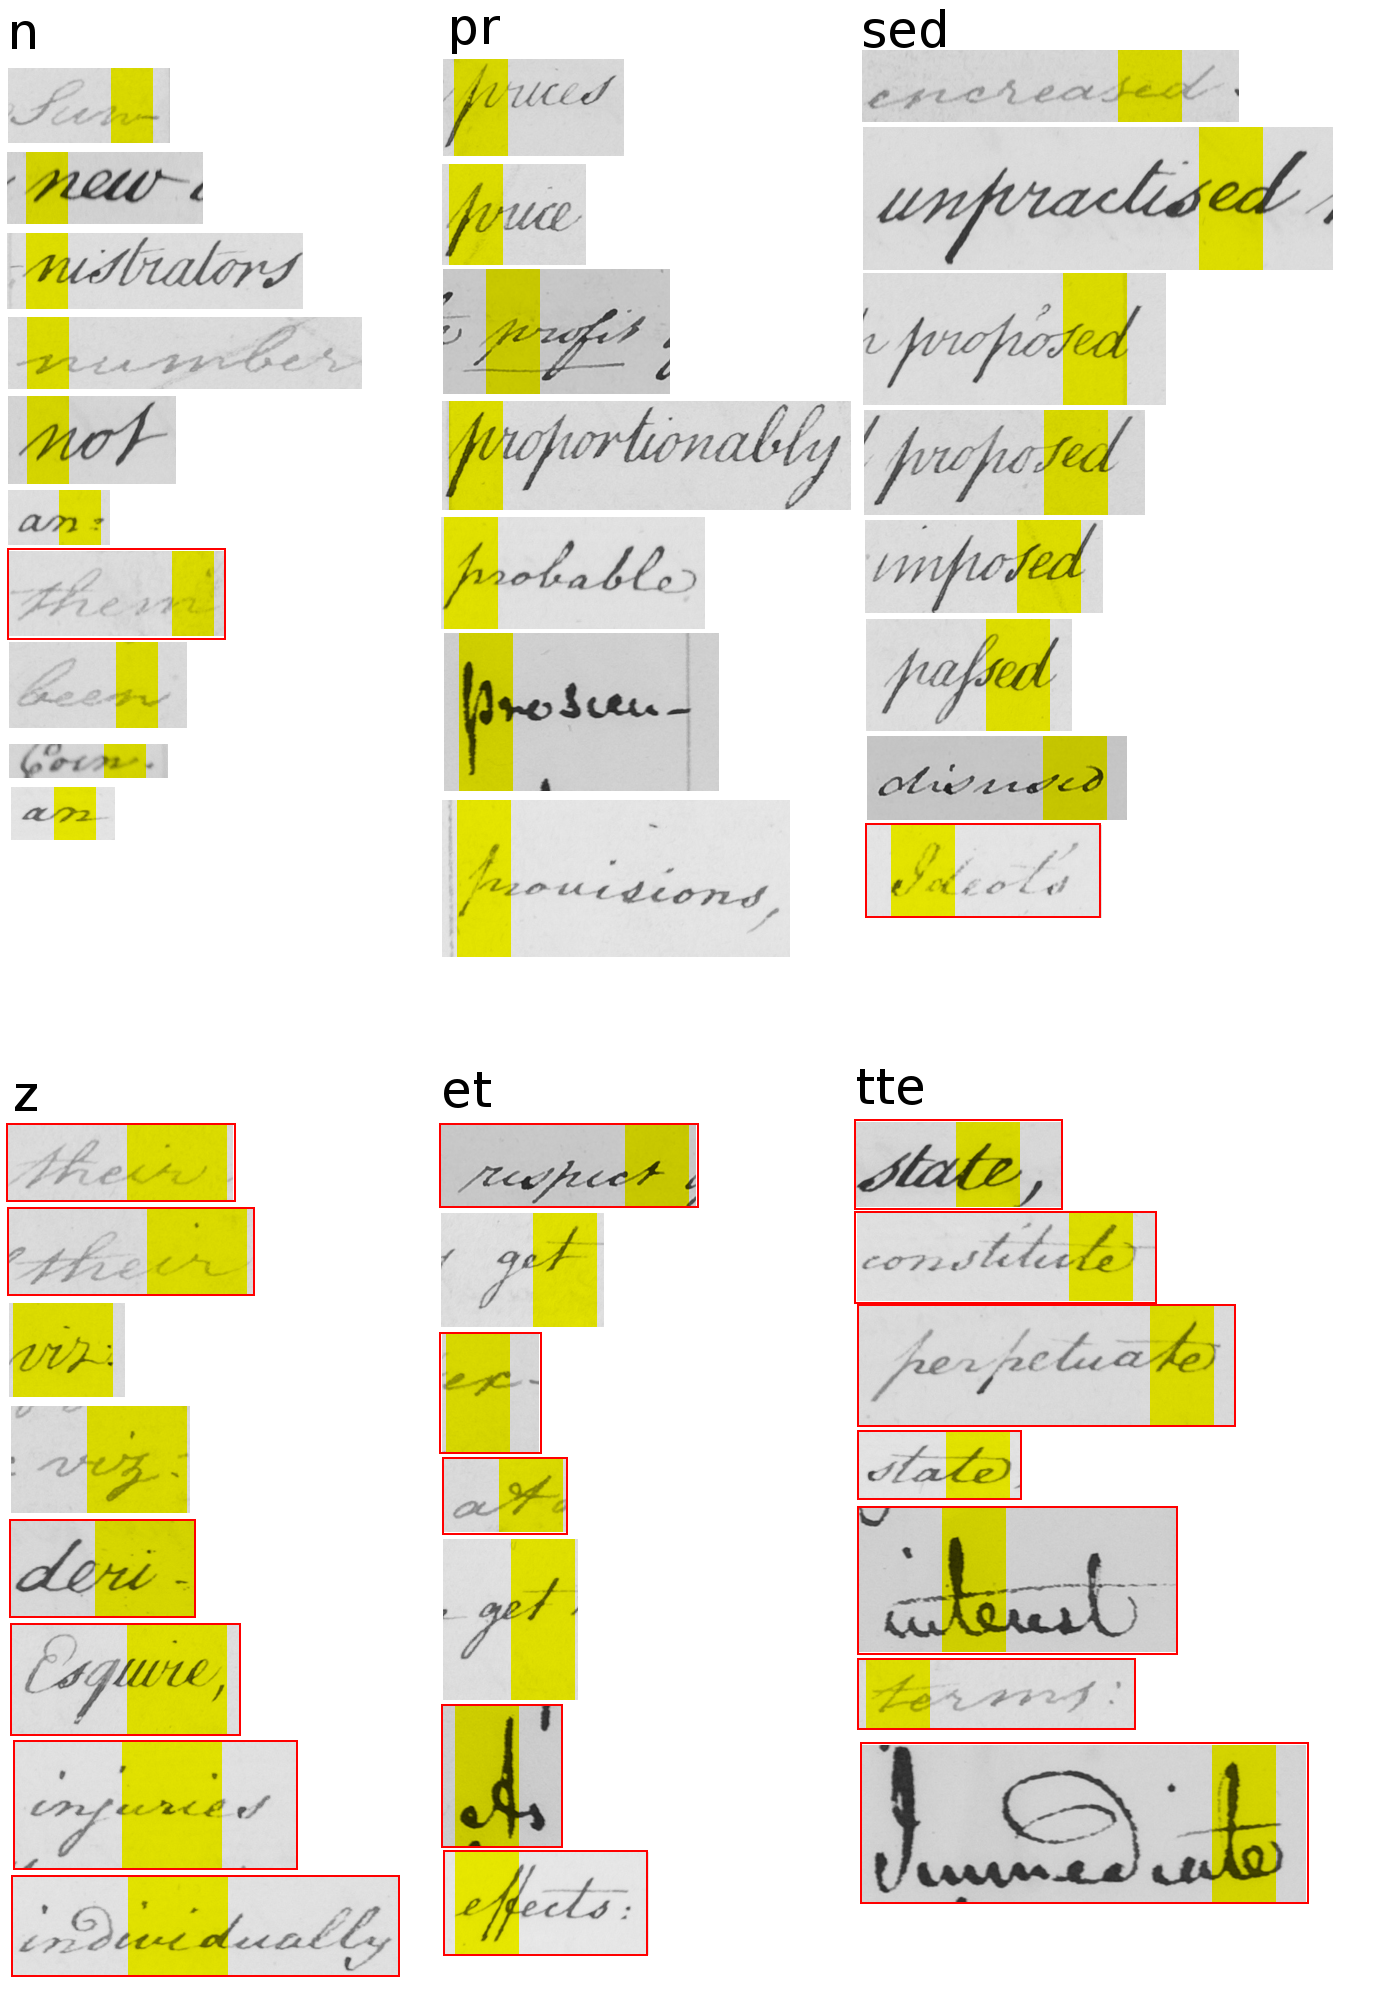
\includegraphics[width=.75\textwidth]{qualSpot}
    \caption{Qualitative results for QbS subword spotting on the Bentham Dataset. Spottings show the top results for the various n-gram queries. We selected some of the better n-grams (`s', `th', `but') and worse n-grams (`j', `et', `tin') by MAP. Red boxes indicate incorrect spottings.
    }
    \label{fig:qualSpot}
\end{figure}

\begin{figure}
    \centering
    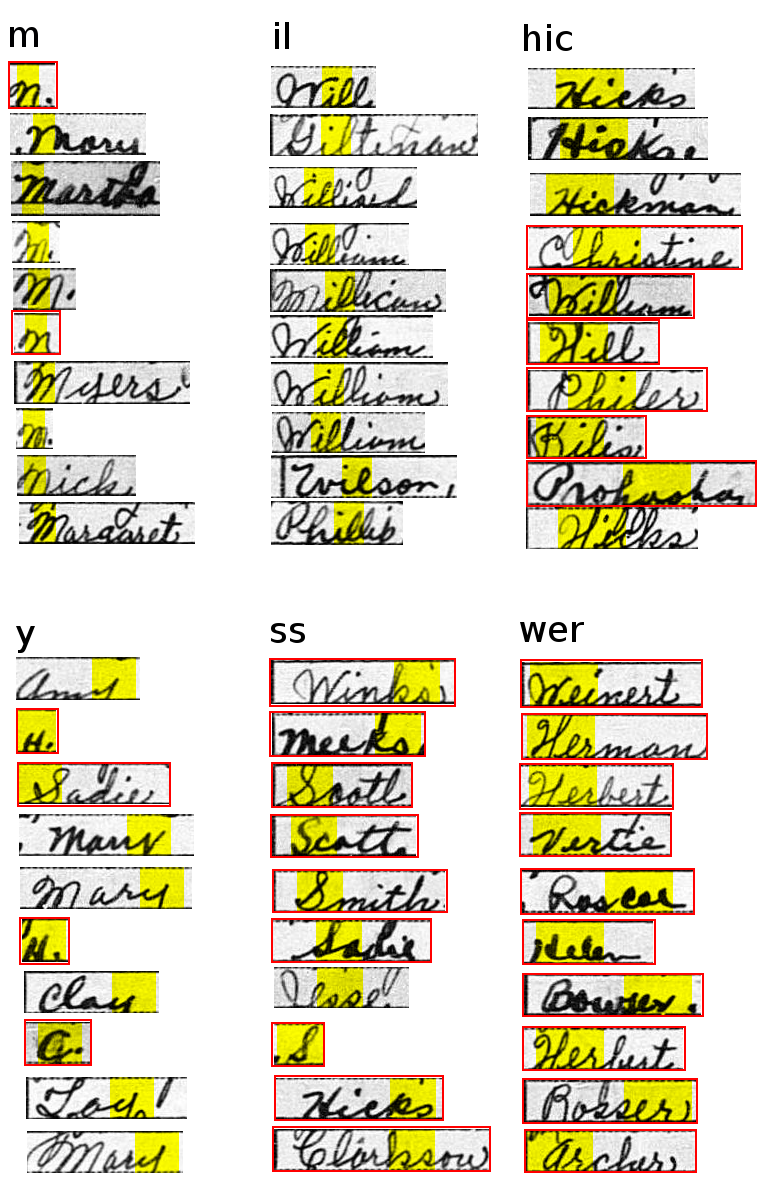
\includegraphics[width=.6\textwidth]{qualSpotNames}
    \caption{Qualitative results for QbS subword spotting on the Census Names Dataset. Spottings show the top results for the various n-gram queries. We selected some of the better n-grams (`i', `el', `int') and worse n-grams (`v', `ts', `pre') by MAP. Red boxes indicate incorrect spottings.
    }
    \label{fig:qualSpotNames}
\end{figure}

In Table \ref{tab:distmetrics} we show a comparison of using cosine similarity and cross-entropy (CE) for PHOC vector comparison using both the original and adapted PHOC vectors. We also show the effect of masking the PHOC vector, where divisions of the word which do not divide evenly with the number of characters being spotted are masked out (e.g.!~division of thirds is masked for spotting bigrams). For QbS, using cross-entropy shows a large improvement over cosine similarity, but cosine similarity always out performs in QbE.

We note that for QbS that the relative performance of unigrams, bigrams, and trigrams is reversed for the Census Names dataset. This occurs becuase of a common error where windows containing only part of the desired n-gram (e.g.~a single character of a bigram) are scored highly. For example...
This exists in the Bentham dataset as well.
The problem becomes most agrevated when trying to spotting n-grams with double letters. As these errors do not occur at all in unigrams, it's MAP is higher. It can occur more freqently in the trigram case than bigram.
We investigated vector comparitors other than cosine similarity becuase of this problem, which is amplified by the fact that cosine-similarity ignores the network's predictions of characters not present in the query; they are multiplied by zero, though they do effect the overall normalization. Cross-entropy reduces the problem as directly penelizes for false positive character predictions.

We note that QbE seems to be relatively immune to this. It is likely due to the fuzziness of the query vector.


%On better QbE with old PHOC:
It is interesting that the best QbE performance is achieved with the original PHOC vector. While it is not totally clear why this is the case, we believe it is becuse a query based on an image is able to more richly describe the word visually with the larger PHOC vector. In a n-gram, different characters have different widths, meaning the location each character in one trigram is slightly different than another trigram. While QbS cannot capture this, QbE with a large enought PHOC vector can.


%We notice in Table \ref{tab:subwordspotting} that on the Census names, unigrams out perform bigrams and trigrams. This immediately seems counterintuitive, as trigrams and bigrams have more context than unigrams. However, n-grams which occur less frequently tend to produce greater error, and the higher n is, the less the n-gram occurs. 
%This can be seen in Figures \ref{fig:benthamsub} and \ref{fig:namessub} and we additionally demonstrated it in Figure \ref{fig:remove}, where trigrams which occur infrequently are removed from our testing set and the MAP increases. This is potentially because there are fewer examples seen in training (training is balanced at a word, not n-gram, level).

%Effect of window size
In Section \ref{detirminewindowsize} we explained how we found the window sizes we used. We show in Figure \ref{fig:windowsizes} the change in MAP as the window size varies for some selected n-grams; an example word image with some windows of varying sizes can be seen in Figure \ref{fig:exampleWindows} to help the reader get a relative estimation of what the window sizes are. As can be seen by the peaks in the data, performance can be dependent on having an optimal window size. We cannot assume however that this is simply becuse the n-grams are becoming fully enclosed in the window; for example, the n-gram ``ery'' (maroon x) has two approximately equal peaks for widths 100 pixels apart. Thus simply measuring the width of the n-grams may yield non-optimal window sizes, we must test the actual performance as done in Section \ref{detirminewindowsize}.

\begin{figure}
    \centering
    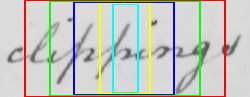
\includegraphics[width=.33\textwidth]{exampleWindows}
    \caption{This shows a word image with windows of various widths: 200-red, 150-green, 100-blue, 50-yellow, 25-cyan.
    }
    \label{fig:exampleWindows}
%\end{figure}

%\begin{figure}
    \centering
    \begin{subfigure}{.99\textwidth}
  \centering
  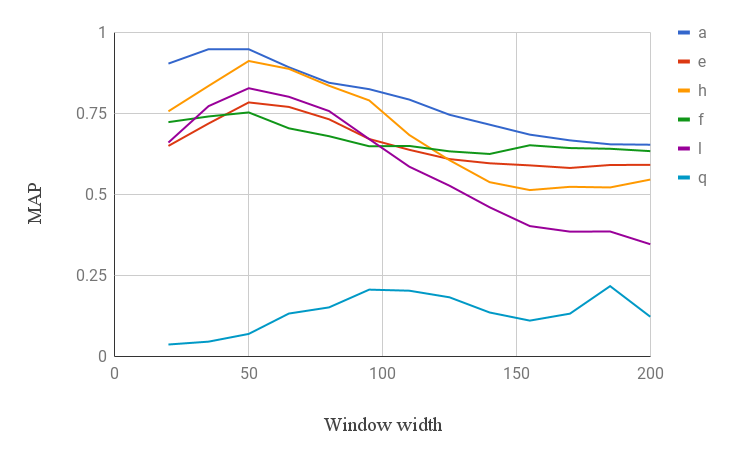
\includegraphics[width=.6\linewidth]{windowsizes1}
  %\caption{Unigrams}
  %\label{fig:benthamUniSpot}
\end{subfigure}
\\
\begin{subfigure}{.99\textwidth}
  \centering
  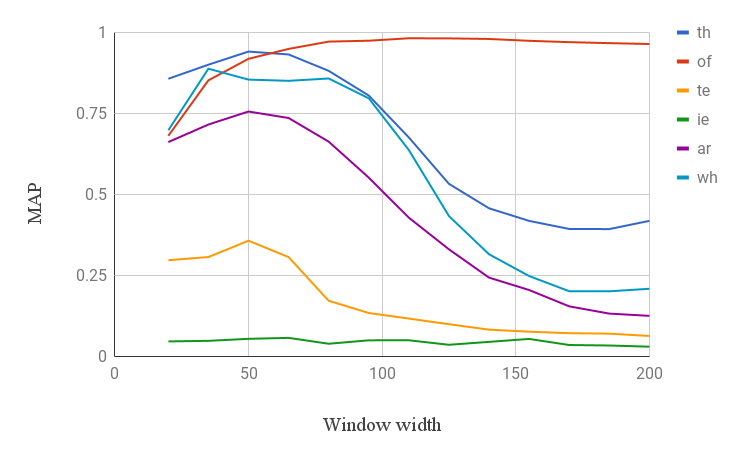
\includegraphics[width=.6\linewidth]{windowsizes2}
  %\caption{Bigrams}
  %\label{fig:benthamBiSpot}
\end{subfigure}
\\
\begin{subfigure}{.99\textwidth}
  \centering
  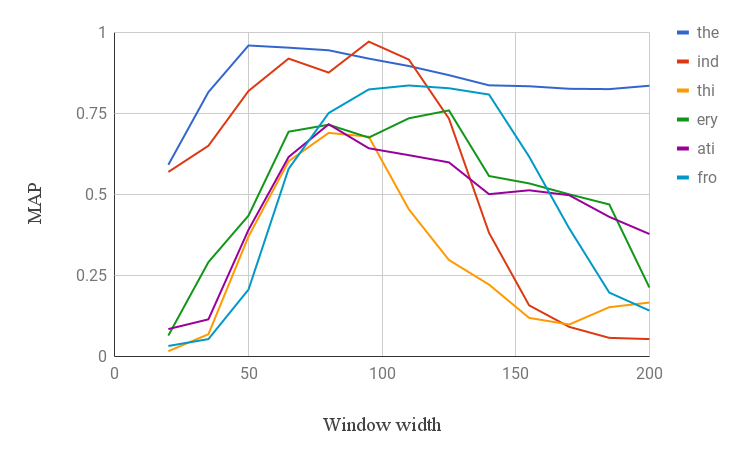
\includegraphics[width=.6\linewidth]{windowsizes3}
  %\caption{Trigrams}
  %\label{fig:benthamBiSpot}
\end{subfigure}
    \caption{These shows the QbS MAP for 18 n-grams on the Bentham dataset for varying sliding window sizes (in pixels). Figure \ref{fig:exampleWindows} shows examples of what these windows might look like.
    }
    \label{fig:windowsizes}
\end{figure}

In Figures \ref{fig:benthamsub}, \ref{fig:benthamsub2}, \ref{fig:namessub} and \ref{fig:namessub2} we show, for the Bentham and Census Names datasets, the average precision of n-grams individually, arranged in descending order of frequency. While there is a general trend of more frequent n-grams being spotted better, there is a wide variance indicating that the distinctiveness of character shape likely plays an important role. We note that many less frequent trigrams are spotted with perfect precision. This is due to there being so few instances (e.g. 4) that with a little bit of luck they can all end up with the top scores. The reverse is also true for the same reason; many less frequent trigrams are spotted with very poor average precision.

\begin{figure}
\centering
\begin{subfigure}{.99\textwidth}
  \centering
  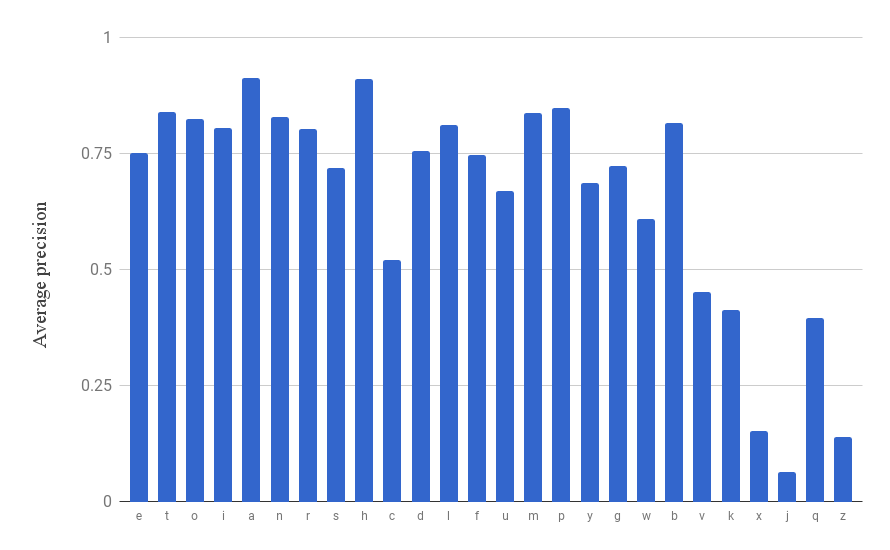
\includegraphics[width=.75\linewidth]{benthamUniSpot}
  \caption{Unigrams}
  \label{fig:benthamUniSpot}
\end{subfigure}
\\
\begin{subfigure}{.99\textwidth}
  \centering
  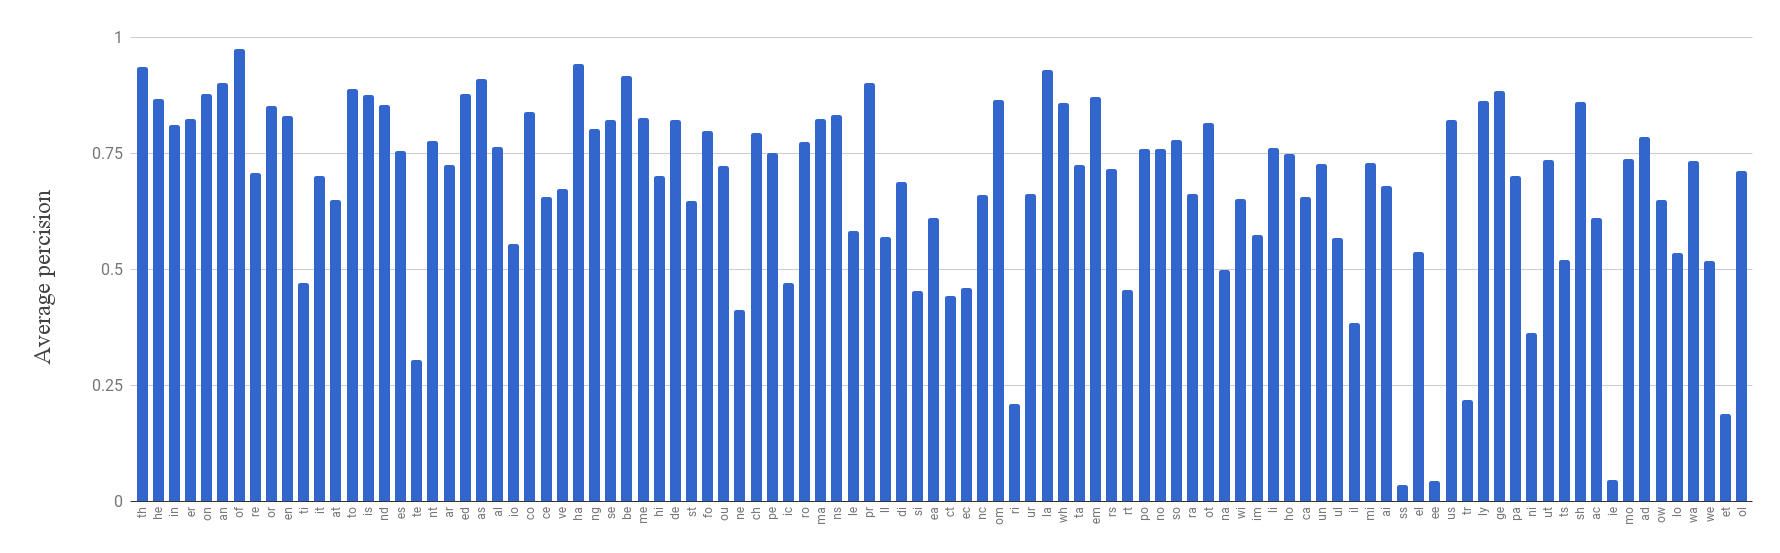
\includegraphics[width=.99\linewidth]{benthamBiSpot}
  \caption{Bigrams}
  \label{fig:benthamBiSpot}
\end{subfigure}
\caption{Results for QbS unigram and bigram spotting on the Bentham dataset. N-grams are arrange in descending order of frequency in test set.}
\label{fig:benthamsub}
\end{figure}

\begin{figure}
\centering
\begin{subfigure}{.99\textwidth}
  \centering
  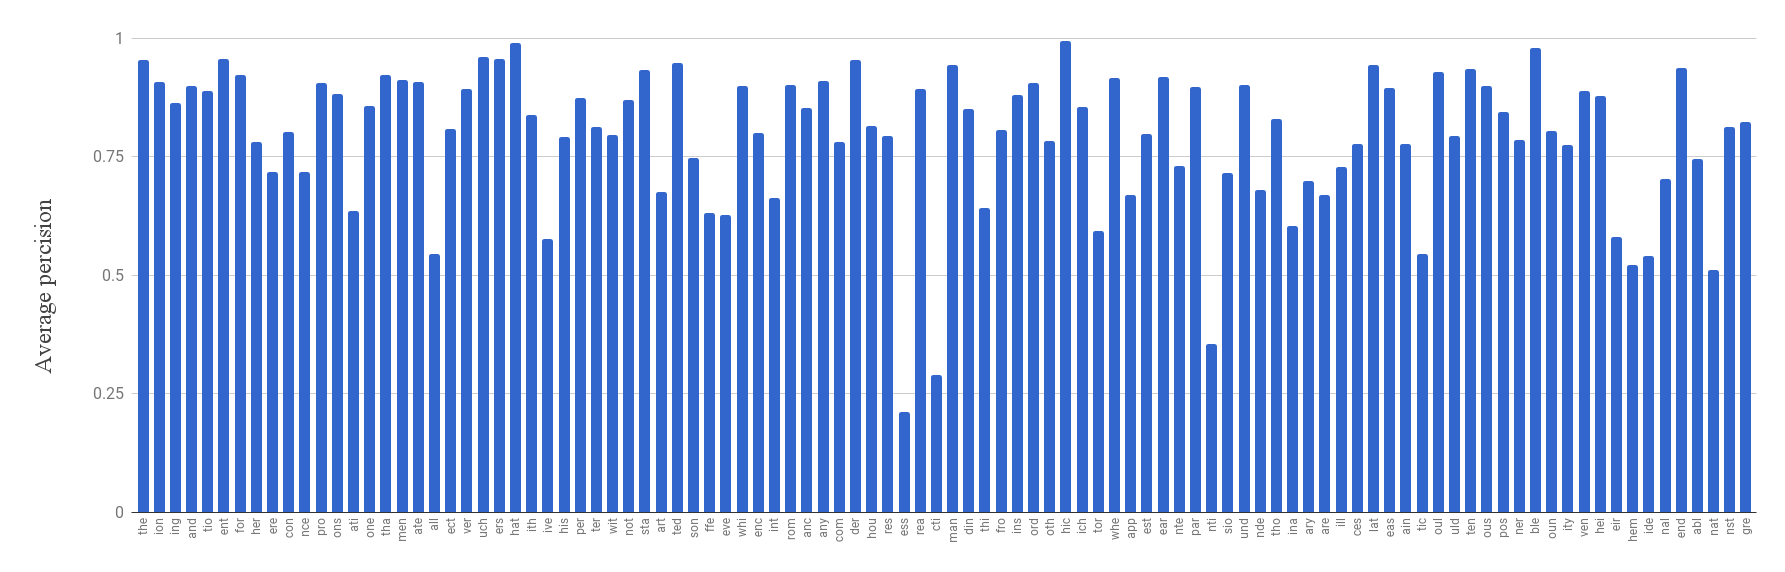
\includegraphics[width=.99\linewidth]{benthamTri1Spot}
  \label{fig:benthamTri1Spot}
\end{subfigure}
\\
\begin{subfigure}{.99\textwidth}
  \centering
  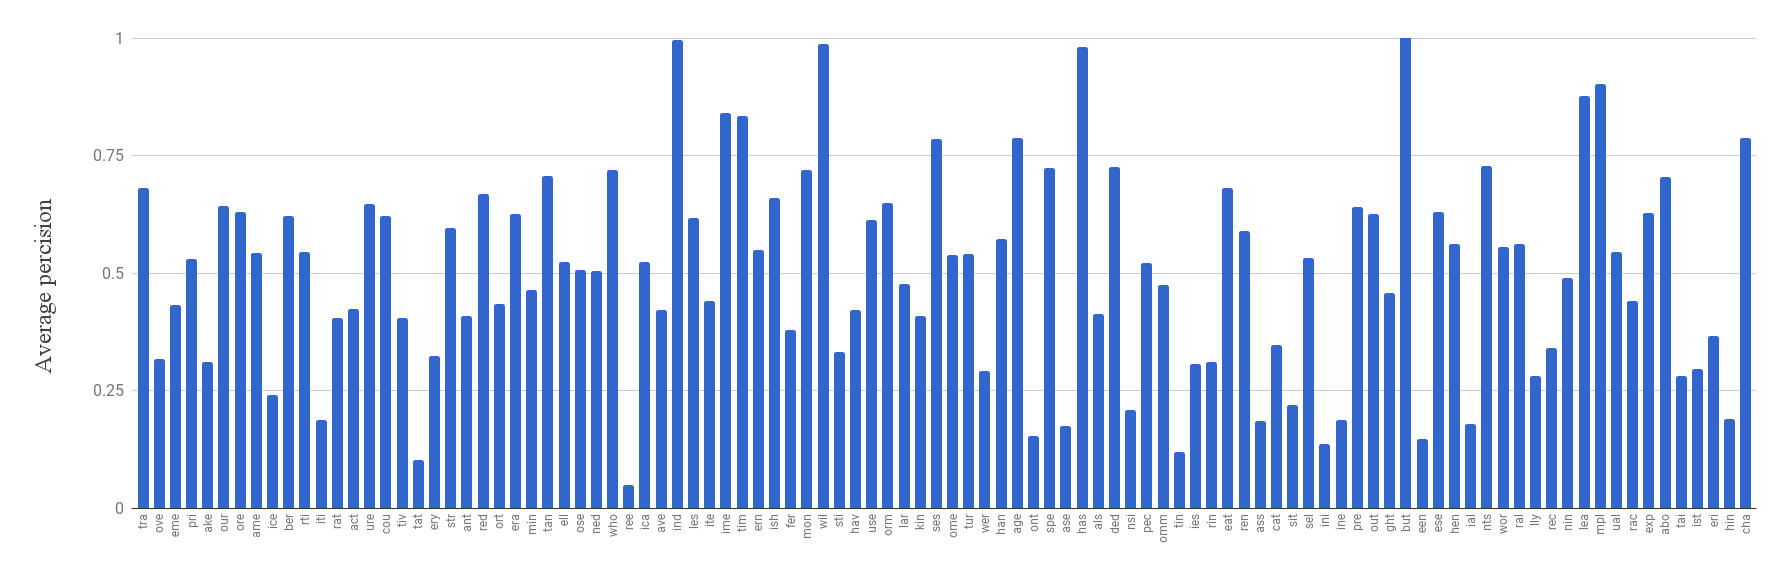
\includegraphics[width=.99\linewidth]{benthamTri2Spot}
  \label{fig:benthamTri2Spot}
\end{subfigure}
\\
\begin{subfigure}{.99\textwidth}
  \centering
  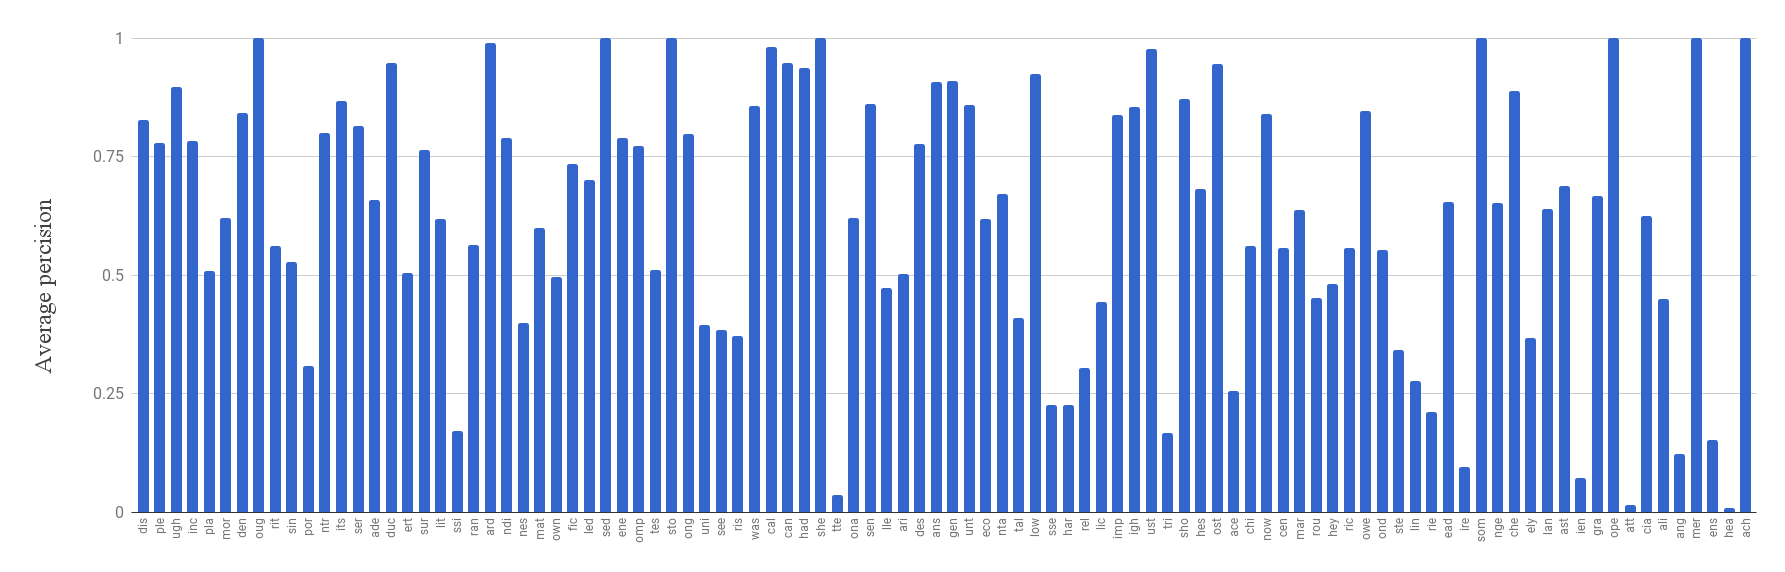
\includegraphics[width=.99\linewidth]{benthamTri3Spot}
  \label{fig:benthamTri3Spot}
\end{subfigure}
\caption{Results for QbS trigram spotting on the Bentham dataset. N-grams are arrange in descending order of frequency in test set.}
\label{fig:benthamsub2}
\end{figure}

\begin{figure}
\centering
\begin{subfigure}{.99\textwidth}
  \centering
  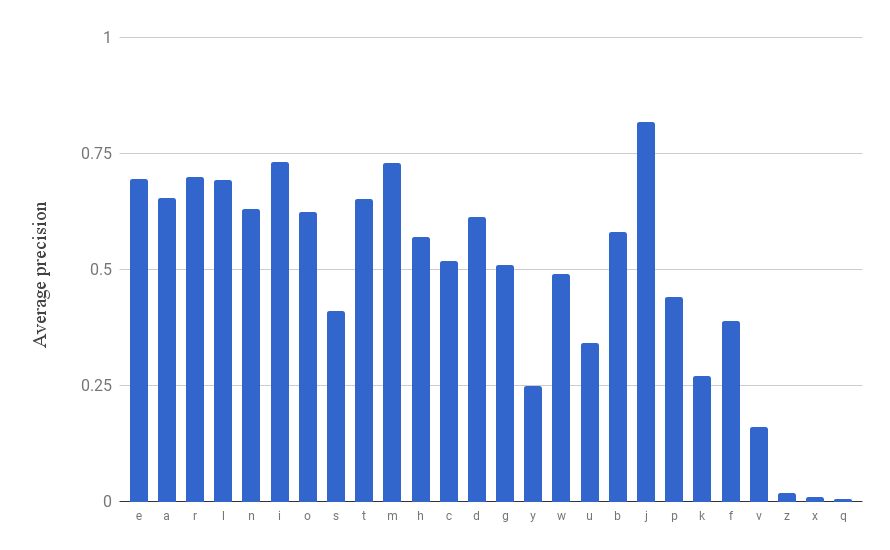
\includegraphics[width=.75\linewidth]{namesUniSpot}
  \caption{Unigrams}
  \label{fig:namesUniSpot}
\end{subfigure}
\\
\begin{subfigure}{.99\textwidth}
  \centering
  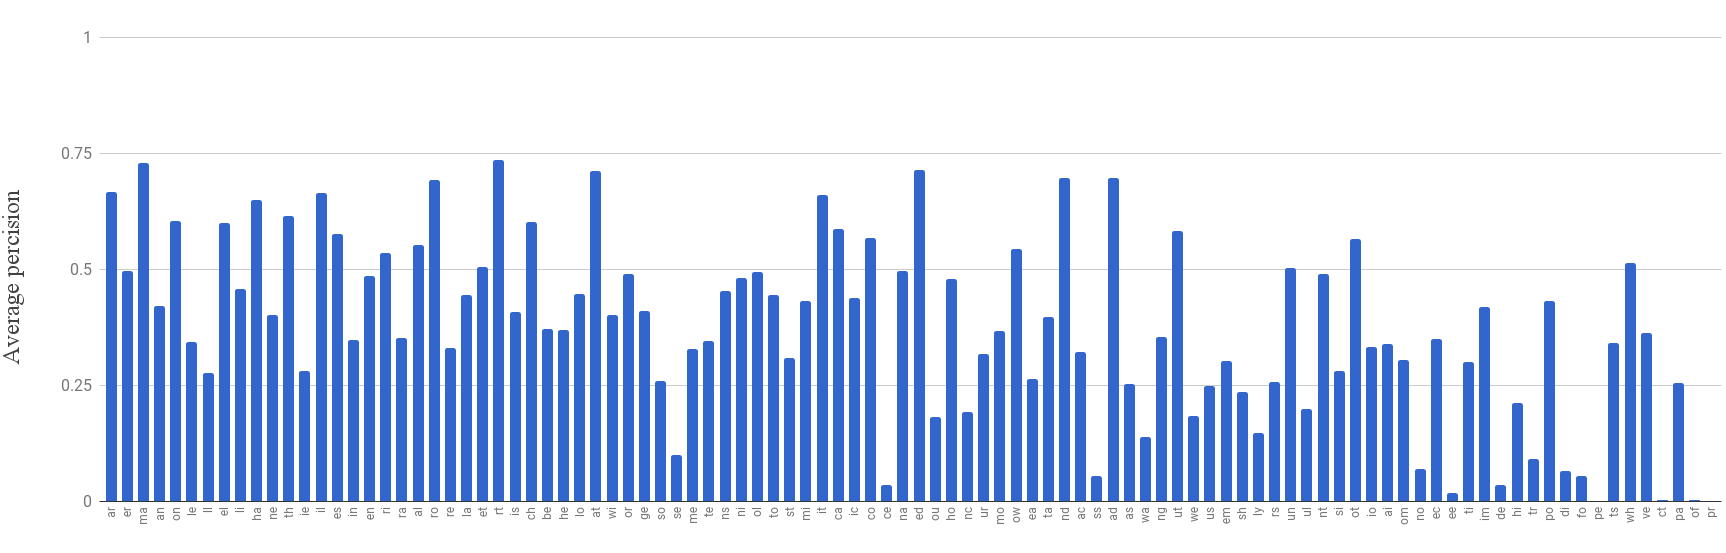
\includegraphics[width=.99\linewidth]{namesBiSpot}
  \caption{Bigrams}
  \label{fig:namesBiSpot}
\end{subfigure}
\caption{Results for QbS unigram and bigram spotting on the Census Names dataset. N-grams are arrange in descending order of frequency in test set.}
\label{fig:namessub}
\end{figure}

\begin{figure}
\centering
\begin{subfigure}{.99\textwidth}
  \centering
  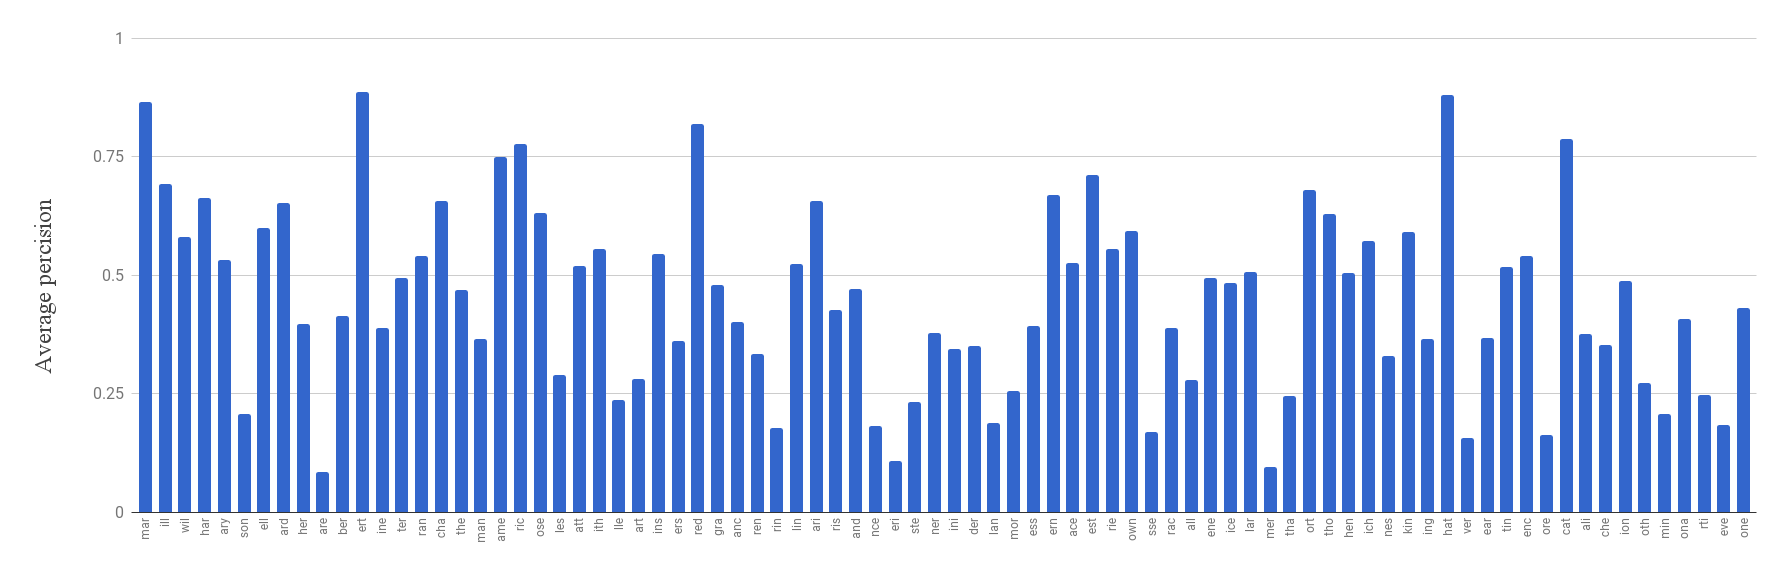
\includegraphics[width=.99\linewidth]{namesTri1Spot}
  \label{fig:namesTri1Spot}
\end{subfigure}
\\
\begin{subfigure}{.99\textwidth}
  \centering
  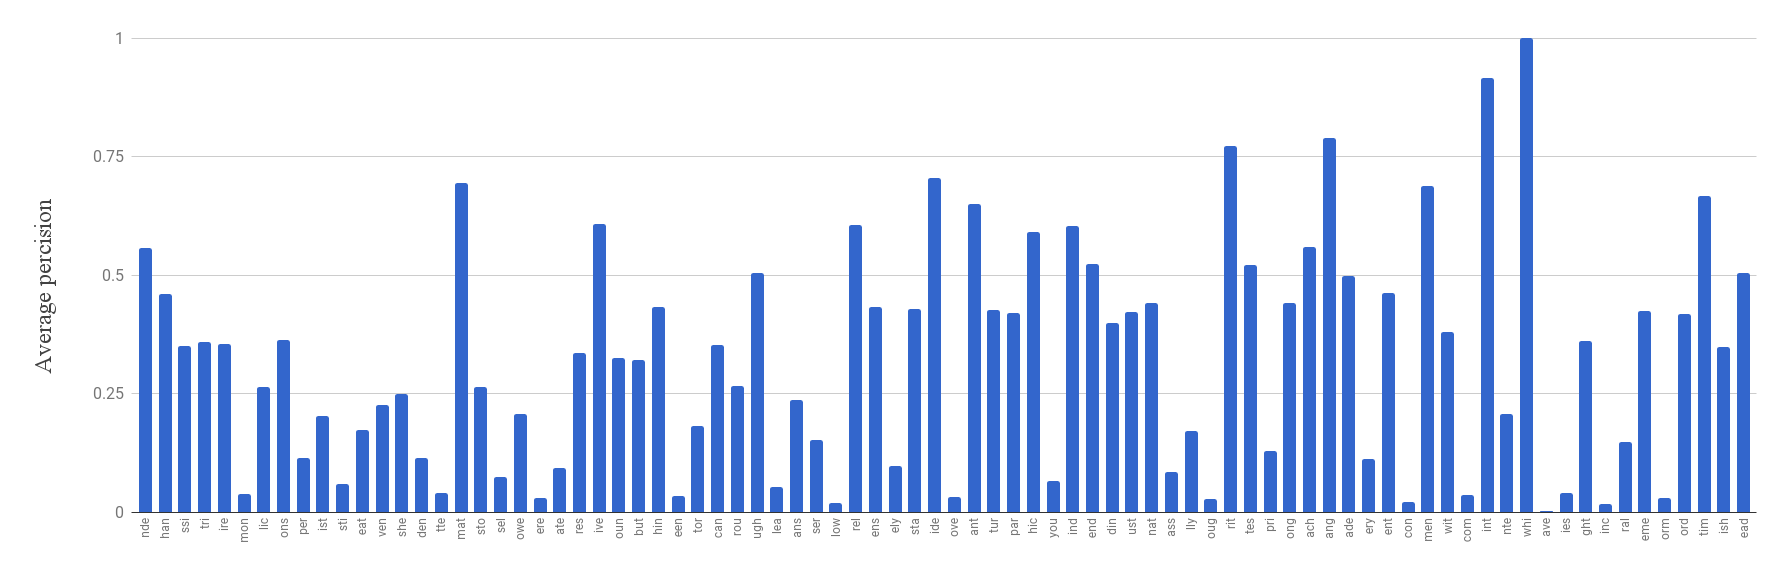
\includegraphics[width=.99\linewidth]{namesTri2Spot}
  \label{fig:namesTri2Spot}
\end{subfigure}
\\
\begin{subfigure}{.99\textwidth}
  \centering
  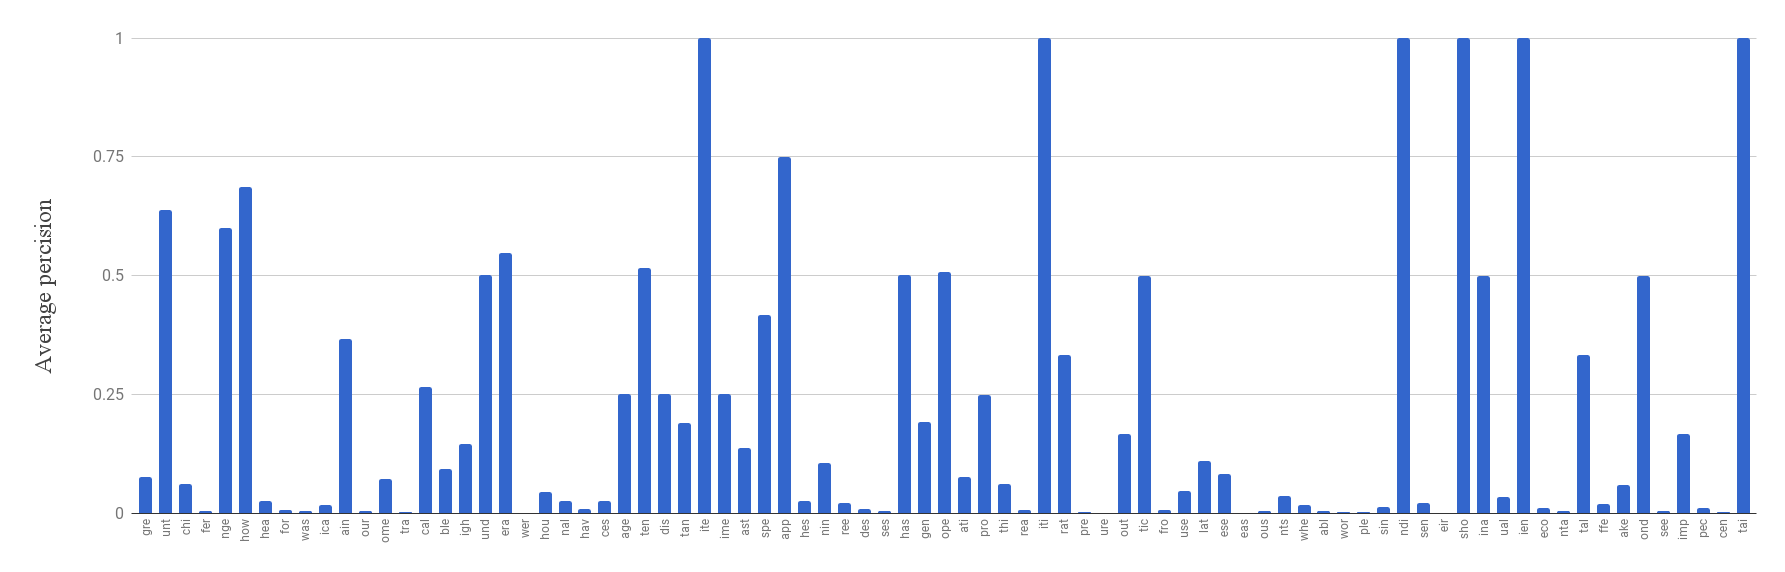
\includegraphics[width=.99\linewidth]{namesTri3Spot}
  \label{fig:namesTri3Spot}
\end{subfigure}
\caption{Results for QbS trigram spotting on the Census Names dataset. N-grams are arrange in descending order of frequency in test set.}
\label{fig:namessub2}
\end{figure}




%\begin{figure}
%    \centering
%    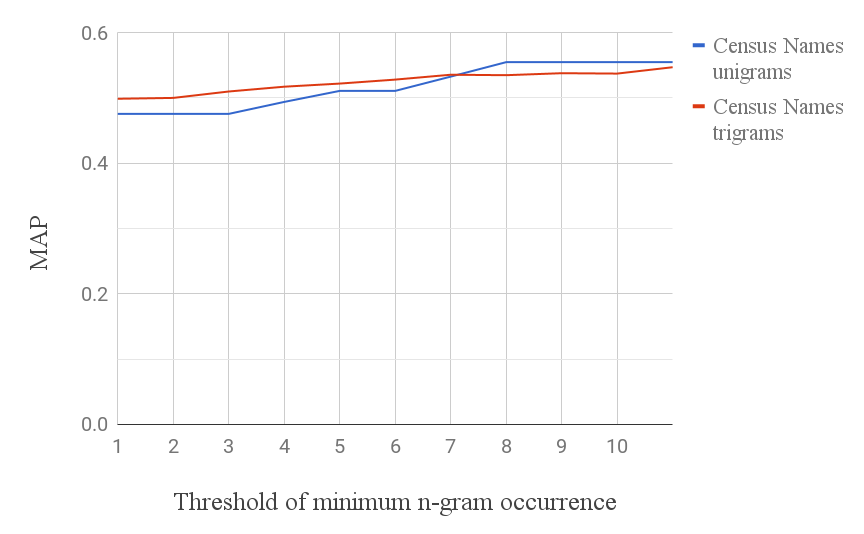
\includegraphics[width=.75\textwidth]{removengrams}
%    \caption{MAP for QbS subword spotting results for trigrams where we only use queries which have an occurrence count above a threshold (in the testing sets). MAP increases as the threshold increases, demonstrating the least frequent n-grams are more difficult. Only trigrams are shown as the effect is more dramatic in these cases. An opposite trend is not observed for uni- or bigrams.
%    }
%    \label{fig:remove}
%\end{figure}





%~/caffe/scripts/cnnspp_spotter/cnnspp_spotter models/phocnet_msfNoLRN_featurizer.prototxt models/phocnet_less_embedderSig.prototxt  net/phocnet_lessNoLRN_iter_144000.caffemodel 1 0.25 ./seg_names_corpus_mod.gtp NAME_COLUMNS/ customWidths.txt manual_segmentations_train_val.csv = ../alphabet.txt ../top100_bigrams_in_freq_order.txt ../top300_trigrams_in_freq_order.txt
%~/caffe/scripts/cnnspp_spotter/cnnspp_spotter models/phocnet_msfNoLRN_featurizer.prototxt models/phocnet_msf_embedderSig.prototxt net/phocnet_msfNoLRN_iter_160000.caffemodel 2 0.25 ben_fixed_corpus.gtp page_images/ customWidths.txt manual_segmentations ! ../alphabet.txt 50 1 1 > respotUni_oct10.txt

\subsection{Respotting Subwords}

We had hoped to use approved spottings as new exemplars for an iterative CAT (computer assisted transcription) system. To verify the validity of this approach we created an experiment where we continually refine spotting results by spotting with new exemplars and merging the results (see Section \ref{combine}). We use the original PHOC vector with cosine similarity as that achieved the best QbE. We show the MAP at each iteration out to 50 iterations in Figures \ref{fig:unigram_respot}, \ref{fig:bigram_respot}, and \ref{fig:trigram_respot}, for uni-, bi-, and trigrams respectively on the Bentham dataset. The first exemplar for an n-gram was selected as the middle score of positive instances from a QbS spotting. The following exemplars were the middle score of the previous QbE spotting's positive instances. We choose to do this as there is a variety of qualities of exemplar images. Taking the middle score should roughly give us a middle quality.
The overall quality of MAP is higher in these experiments as we only used n-grams which occur at least 100 times, which tend to be the easier instances.
We can see that the iterative refinement leads to better results compared to the average of all the QbE scores for the individual 50 queries, except in the case of trigrams. This is unusual given the average QbE scores are relatively high compared to the QbS score. However, for all n-grams the combine QbE results underperforms QbS; we do not include QbE as part of our CAT system.
%It appears that aggregating multiple queries tends to stabilized the bad queries.%, though it does not out perform QbS (except with trigrams) or individual good QbE queries (as the spikes in performance are not at the end).

\begin{figure}
    \centering
    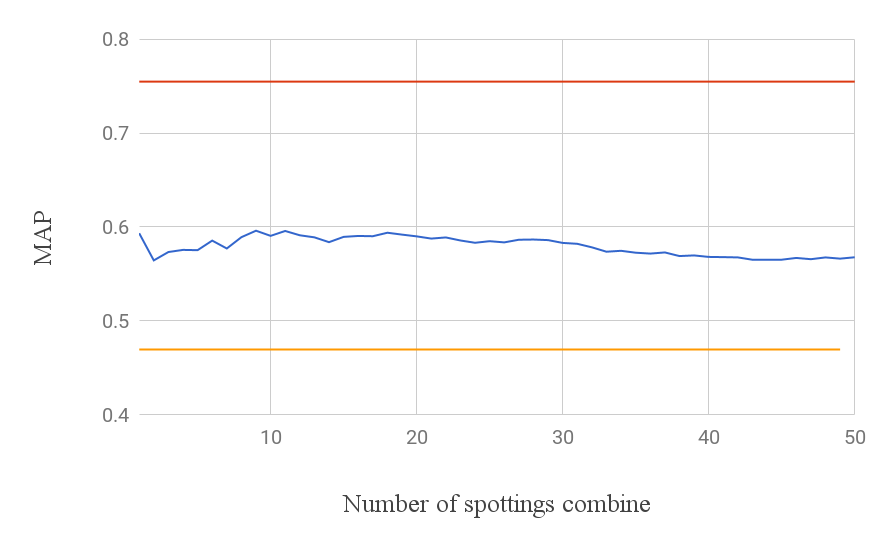
\includegraphics[width=.75\textwidth]{unigram_respot_chart}
    \caption{Unigram MAP when spotting results of consecutive image queries are combine (blue). The red line represents QbS performance and the yellow the average performance of all 50 QbE queries.}
    \label{fig:unigram_respot}
\end{figure}
\begin{figure}
    \centering
    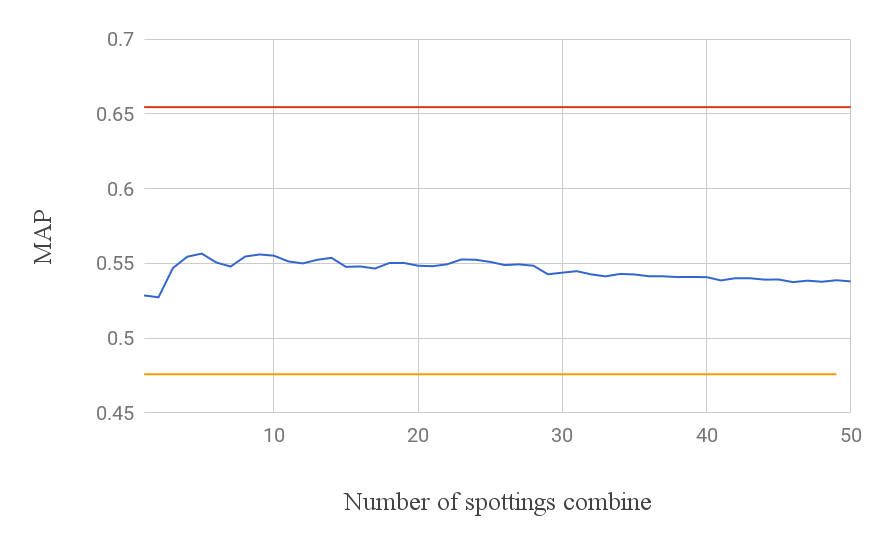
\includegraphics[width=.75\textwidth]{bigram_respot_chart}
    \caption{Bigram MAP when spotting results of consecutive image queries are combine (blue). The red line represents QbS performance and the yellow the average performance of all 50 QbE queries.}
    \label{fig:bigram_respot}
\end{figure}
\begin{figure}
    \centering
    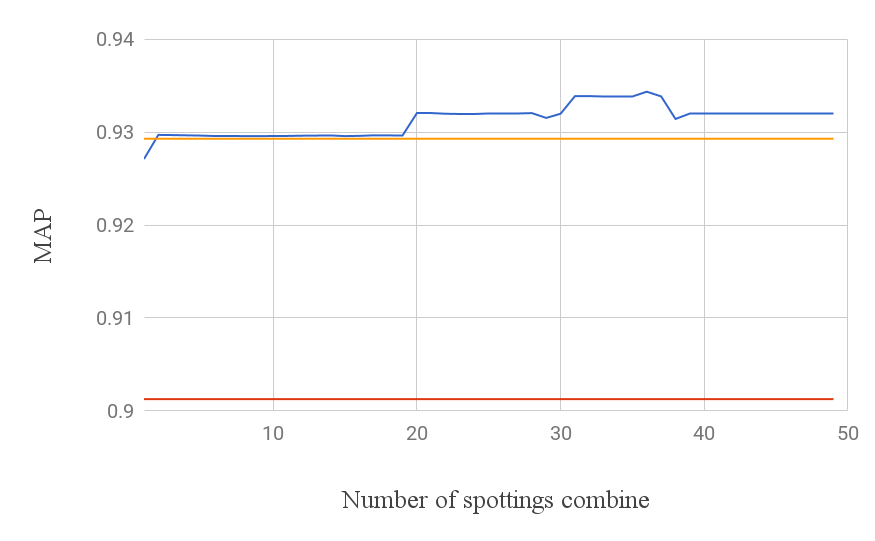
\includegraphics[width=.75\textwidth]{trigram_respot_chart}
    \caption{Trigram MAP when spotting results of consecutive image queries are combine (blue). The red line represents QbS performance and the yellow the average performance of all 50 QbE queries.}
    \label{fig:trigram_respot}
\end{figure}




%%%%%%%%%%%%%%%%%%%%%%%%%%%%%%%%%%%%%%%%%%%%%%%%%%%%%%%%%%%%%%%%%%%%%%%


\chapter{Applications of Subword Spotting}\label{applications}

In this chapter we explain two applications of subword spotting: assisting persons manually transcribing document images and suffix spotting. Due to its complexity, we explore using subword spotting to transcribe in the next chapter.

\section{Manual Transcription Assistant}
Frequently when a person is transcribing a handwritten document they come across a handwritten word they do not recognize. A common solution is to scan the document for similar shapes which are present in the difficult word. If the transcriber can find the same letters, written by the same author, in the context of a word they do recognize, the transcriber can identify the letters, thus aiding in the transcription of a difficult word. 
However, the same letters may be time consuming to find due to the density of the document and rarity of the characters. QbE subword spotting provides a way to automate this scanning task. The user need only to select the portion of the difficult word they wish to query with and the system can return a ranked list of results.
We are able to achieve real-time results over a handful of pages by using word segmentations and pre-computing PHOC vectors for a set of reasonible window sizes at 16  pixel strid. We snap users query is snapped to. 

Figure \ref{fig:assist_demo} demonstrates how the assistant works. First the unrecognizzed characters are selected (a), in this case a  ``G'', and the bounding box is snapped to the precomputed one. This PHOC vector is compared against all others of the same window size. The ranked list is shown to the user both as a list (c) and by highlighting the results with the color intensity representing the strength of the match (b). Suppose that the top results aren't words the user is familiar with, but the user recognizes the ``G'' in the first result (blue arrow, ``Gash''). By selecting it, the system performs a QbE search, combining the results with that of the original query using the method described in Section \ref{combine}. In the combine results (e) the word ``Grace'' (a more recognizible word) has moved to the third spot .

%If further refinement is desired, e.g.~the top true instances returned are in isolation as well,
\begin{figure}
    \centering
    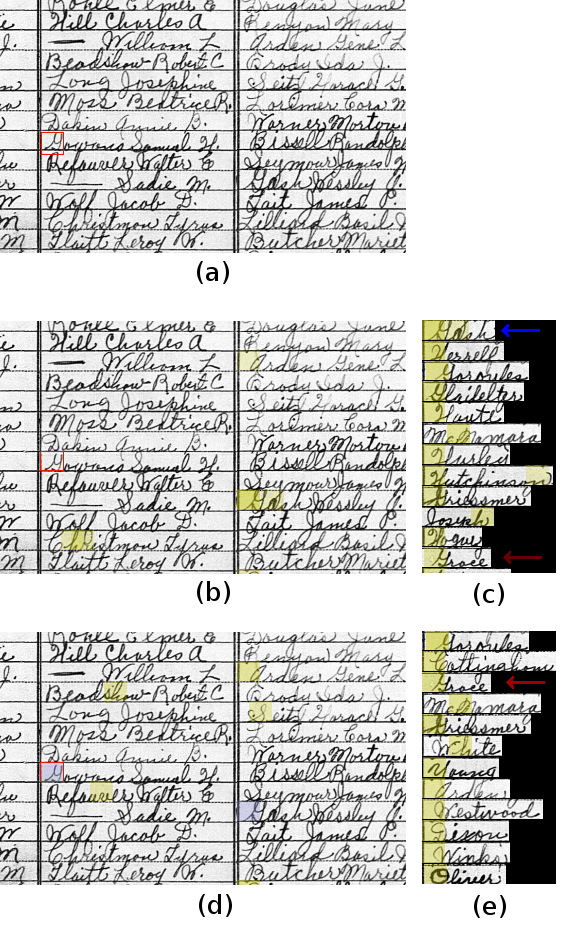
\includegraphics[width=.65\textwidth]{assist_demo}
    \caption{Transcription assistance using subword spotting. (a) The user selects an unknown character (``G'', red box) to search the documents. (b) The results of a QbE search are displayed, strength of highlight relative to spotting score. (c) A ranked list of matches is shown (best match at top). The user selects another instance to refine the results (blue arrow). (d) Combined QbE results. Exemplars are highlighted in blue. (e) Ranked combined results, a more common word, ``Grace'' (red arrow), has moved up to a more visible position.}
    \label{fig:assist_demo}
\end{figure}

This assistant system is a proof of concept and no testing was done on it. Its performance is directly related to the QbE performance reported in Table \ref{tab:subwordspotting}.

%Speed considerations, we optimize, but work is being done on fast CNN execution

\section{Suffix Spotting}
Word spotting is a technique that can be used to find certain words in a corpus of handwritten documents. However, there are certain situations where one may want to search for a partial word, such as a prefix or suffix. For example, if one wanted to find names of towns in a corpus of German documents, spotting words with the suffix ``-berg'' should return many town names.

We identified a list of 41 suffixes and evaluate spotting the suffixes present from this list in the IAM and Census Names dataset. 
 The window size for a given suffix query is found by identifying all n-grams we have window estimates for (see Section \ref{detirminewindowsize}) which compose the query and averaging their window widths according to which characters they contribute to.
We are able to make the assumption that the spottings only occur at the end of the word which reduces the number of possible subwindows significantly. We additionally don't need to consider window overlap in our evaluation as the goal is whole word retrieval.

We evaluate QbS suffix spotting on the IAM and Census Names datasets as these have a reasonable number of instances of our suffixes. We achieved a MAP of 0.583 for the IAM dataset and a MAP of 0.488 for the Census Names dataset. We show the AP for the suffixes individually in Figures \ref{fig:IAM_suffix} and \ref{fig:names_suffix}. Note that the suffixes achieving 100\% AP occur only once or twice. For the IAM dataset the suffixes occur about half the time as the whole words, meaning it may not represent subword spotting as well as the Census Names dataset, which had only one instance of a subword being a whole word (name).



%\begin{table}
%\centering
%\begin{tabular}{| l | c  c |}
%  \hline
%   & IAM & Census Names\\
%  \hline			
%  %oldMAP across queries & 0.481  & 0.271\\
%  %oldMAP across instances & 0.581 & 0.338\\ 
%  MAP across queries & 0.550  & 0.297 \\
%  MAP across instances & 0.660 & 0.403 \\
%  \hline  
%\end{tabular}
%\caption{MAP for suffix spotting results using QbS.}
%\label{tab:suffixspottingresults}
%\end{table}

\begin{figure}
    \centering
    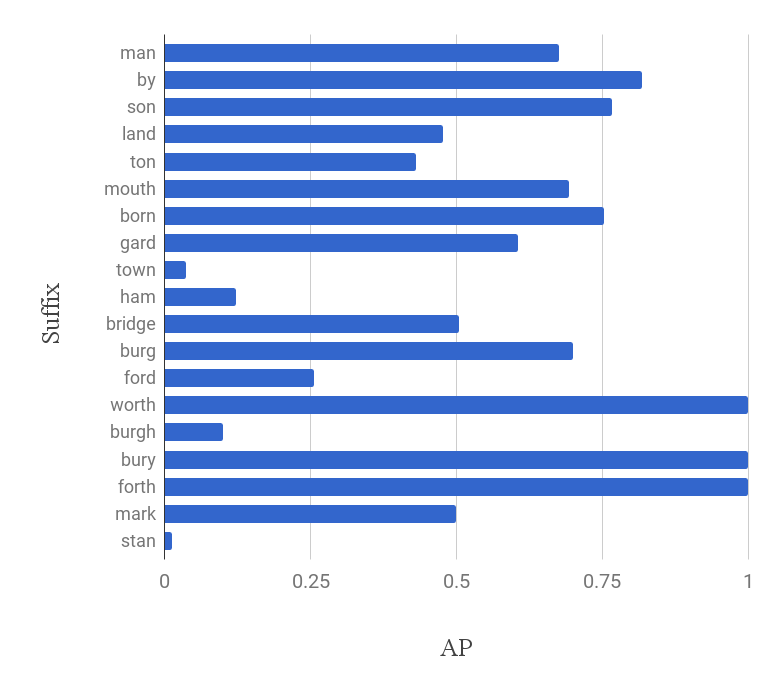
\includegraphics[width=.75\textwidth]{suffix_IAM_ap}
    \caption{Suffix spotting AP of individual suffixes for the IAM dataset. Arranged in descending order of frequency in test set.}
    \label{fig:IAM_suffix}
\end{figure}

\begin{figure}
    \centering
    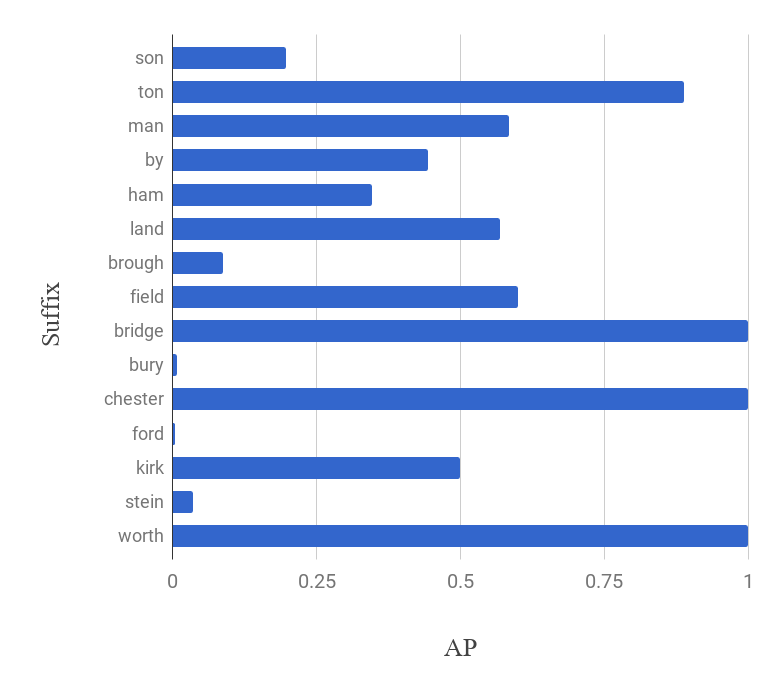
\includegraphics[width=.75\textwidth]{suffix_names_ap}
    \caption{Suffix spotting AP of individual suffixes for the Census Names dataset. Arranged in descending order of frequency in test set.}
    \label{fig:names_suffix}
\end{figure}

%The MAP for the Census Names dataset reflects its subword spotting performance. We can see in Figures \ref{fig:IAM_suffix} and \ref{fig:names_suffix} that more frequent suffixes perform more consistently, while less frequent suffixes have more variability in performance.




\chapter{Application of Subword Spotting to Transcription}\label{transcription}

Subword spotting can also be used to transcribe words. There are several ways one could do this, but one of the key aspects that makes subword spotting for transcription appealing is that while subword spotting naturally yields partial transcriptions, matching against a lexicon can constrain the full transcription from a partial one. We aim towards a CAT (computer assisted transcription) model to better leverage the possibility of user feedback on the steps leading to the full transcription.

We describe 4 transcription methods in this chapter and the results in the following chapter.
For all methods we used a lexicon. Our primary lexicon consists of 108,028 words and 6,939 names, as described in Chapter \ref{datasets}.

\section{Baseline: CAT Through PHOC Vectors}
%Knowledge::Corpus::phocTrans
We use a nearest-neighbors approach as a baseline to transcription using our spotting network, similar to what \cite{krishnan2016} do for word recognition. The PHOC vectors generated by the network on word image are compared to the PHOC vectors of the  words in our lexicon using a cosine similarity and the top N matches from the lexicon are returned. This does not use subword spotting, and thus provides a baseline for transcription using our PHOCNet based architecture.

To compare it to the other CAT methods, we assume a transcription for a word image is performed by a user selecting the correct transcription from the top 7 returned lexicon words. If the correct transcription is not returned in the top 7, it must be manually transcribed.
To be more efficient, we only return a certain portion of the words to be transcribed in this manner (the remainder needing manual transcription). This portion is selected by ordering words according to the mean score of the top 7 lexical matches.







\section{CAT Through Approved Subword Spottings}

%overview, and image
\begin{figure}
    \centering
    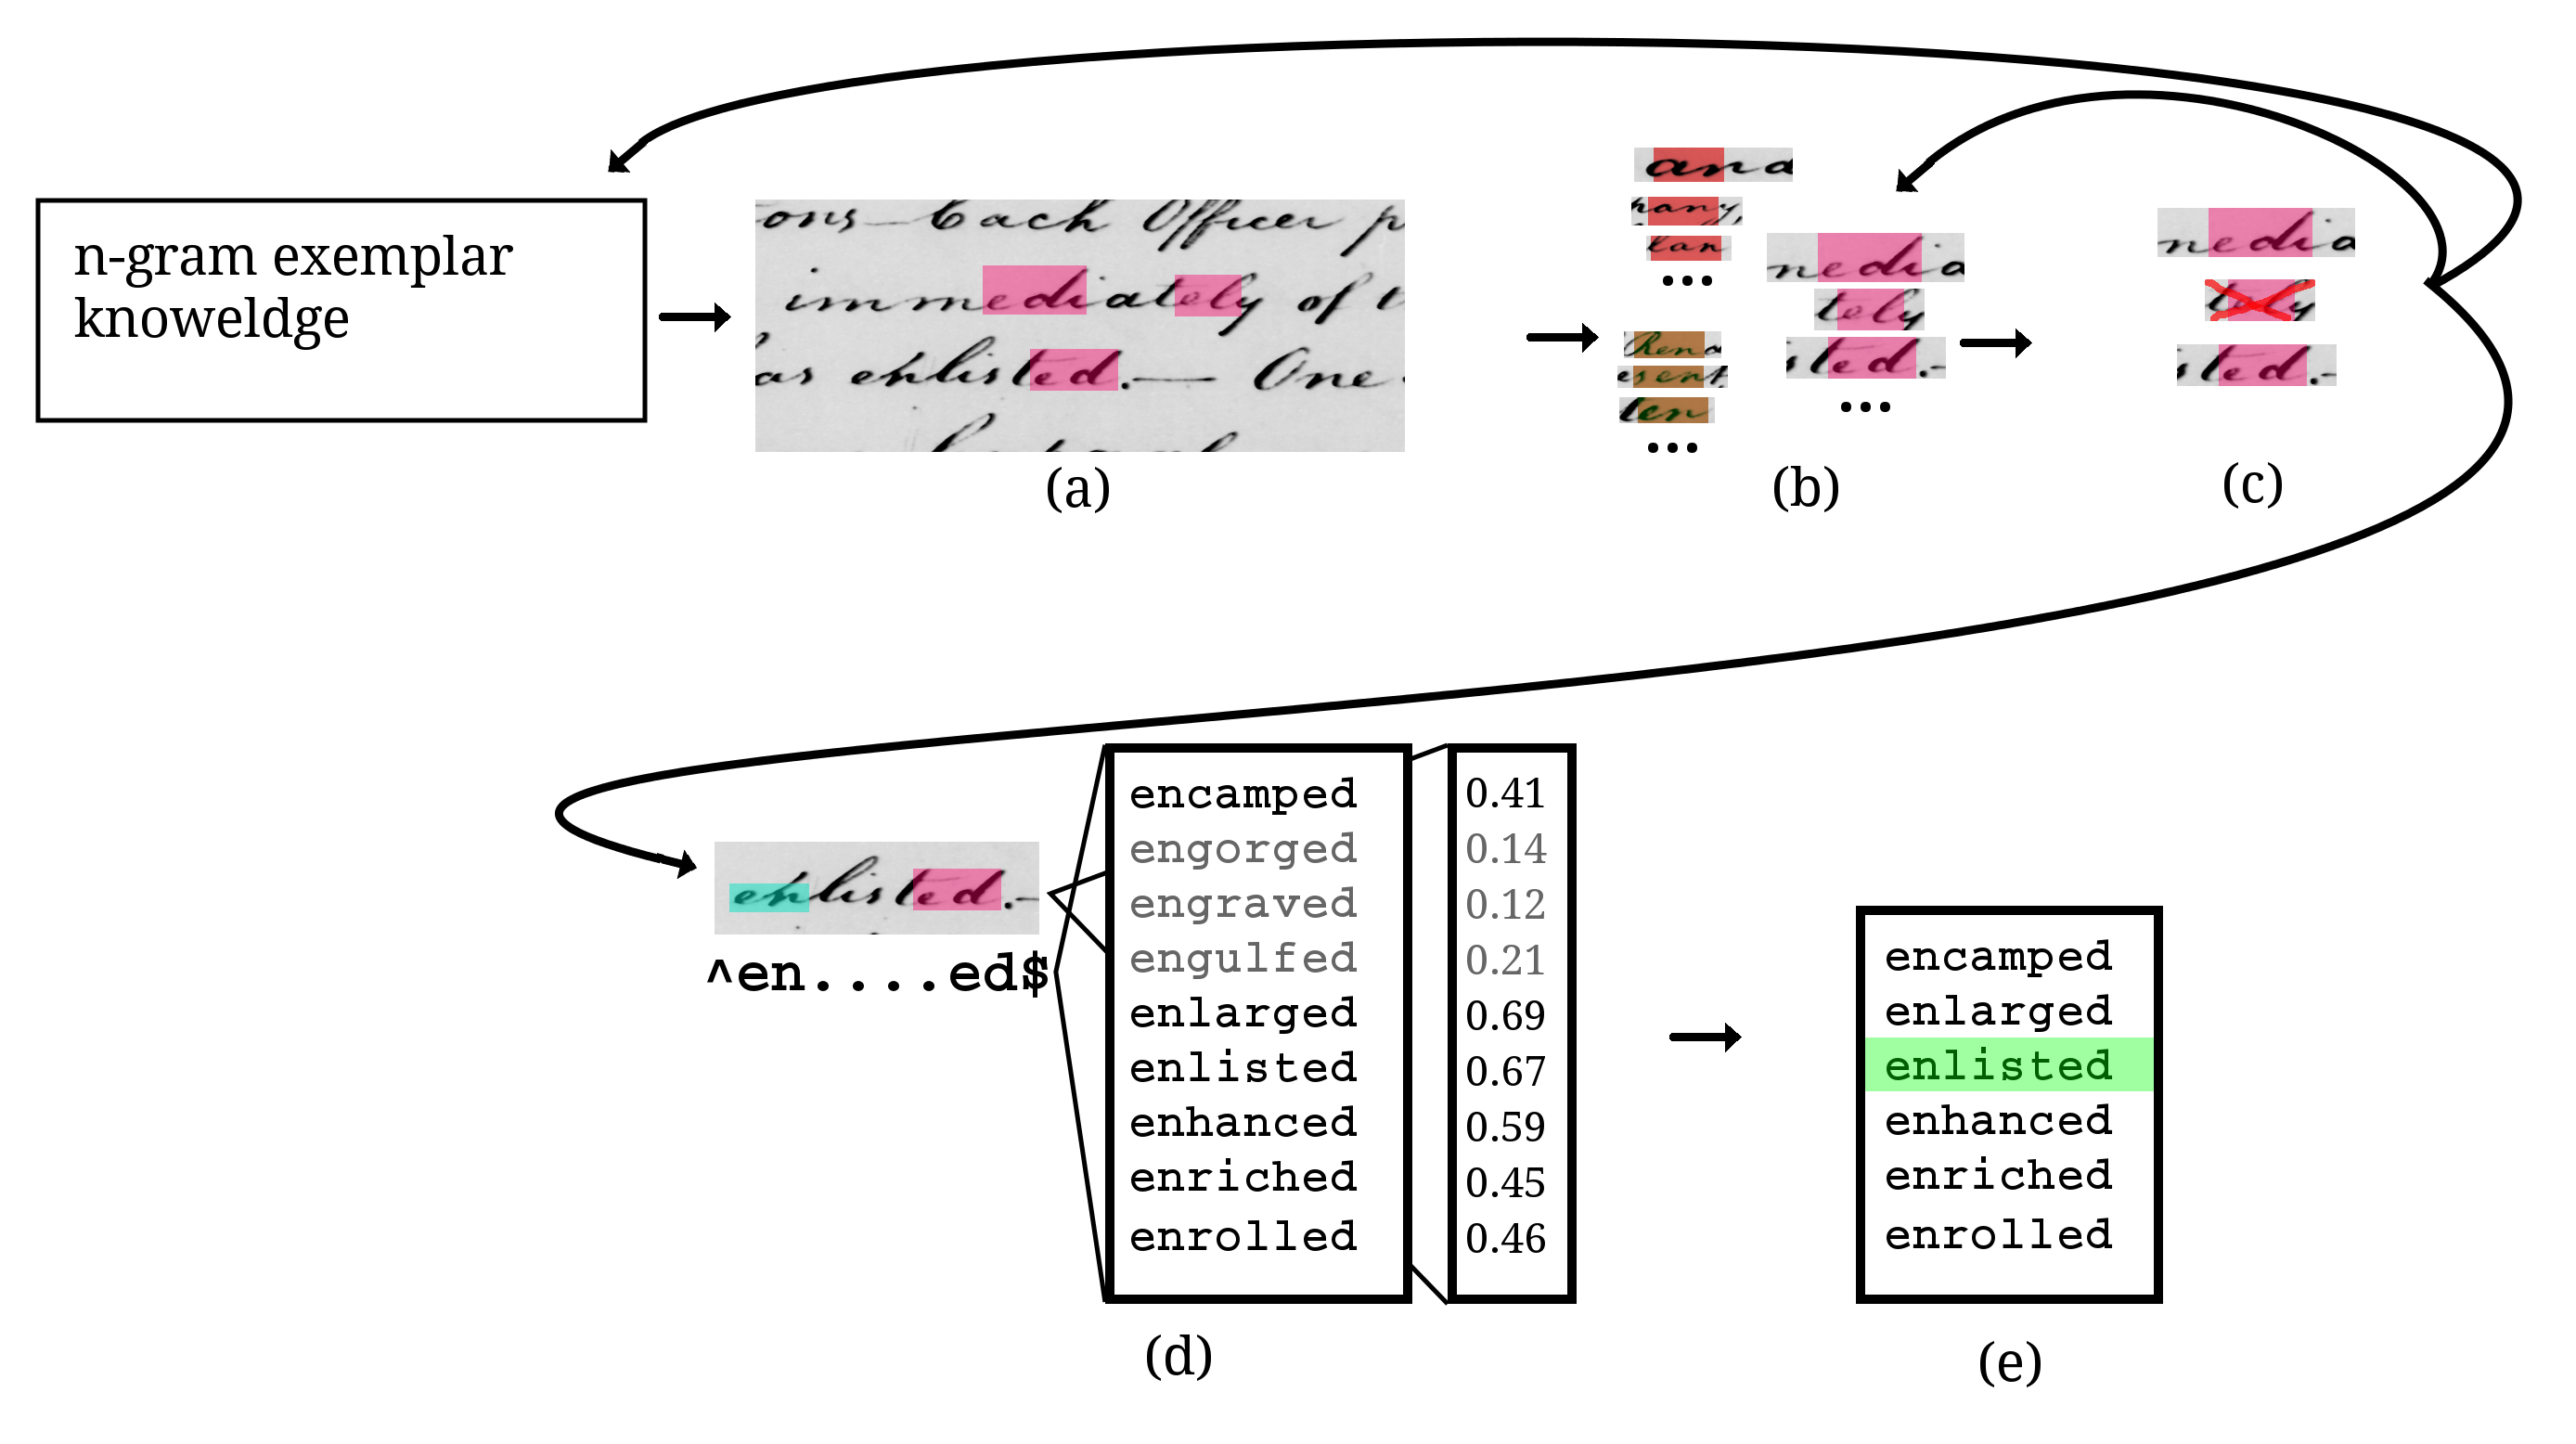
\includegraphics[width=.9\textwidth]{flow6}
    \caption{An overview of the CAT system which uses approved subword spottings. The arrows represent the flow of data. (a) Subword spotting is performed. (b) Spotting results are sorted an distributed as batches. (c) Users classify the spottings. (d) The spottings are aggregated into a regular expression. This yields a set of possible transcriptions in the lexicon. These are scored with word spotting on the word image. (e) The (reduced) list of possible transcriptions is sent to a user to selects the correct one.}
    \label{fig:flow}
\end{figure}
An overview of the CAT system using approved subword spotting can be seen in Figure \ref{fig:flow}.  Initially the system spots character n-grams in the corpus of word images (a). These results are pooled and sent to users in batches (b). After the user identifies correct/incorrect spottings (c), the spottings' labels and positions in the word images are used to create regular expressions which is used to query a lexicon for a list of all words matching the constraints set by the spottings (d). These are scored through word spotting (spotting each lexically relevent word in the image) and lower scores are removed from the list (according to an Otsu threshold). This list is then sent to a user, who selects the correct transcription (e). Information from approved spottings is used in further spottings.

When there are no more user tasks the system is finished. Words not transcribed will need to be manually transcribed.

We now go over the individual pieces in greater detail.

\subsection{Subword Spotting}
We follow the same procedure for subword spotting as outlined in the Chapter \ref{subwordspotting}. We begin by spotting the n-grams using QbS. We evenly interleave spotting the n-grams, ordering each n by frequency order. That is, we order all trigrams, bigrams and unigrams individually by frequency order, then interleave these three lists such that each list is evenly disperesed among the resulting list. 

We attempted to use QbE after spottings are approved as correct by users. We combine QbE results as described in Section \ref{combine} when we had a certain threshold of approved spottings (to ensure stability). However, this did not enhance performance so we did not include this in our final tests.

To reduce the number of possible n-grams needing approval, we only return the top portion of all subwindows for a spotting: 75\% for unigrams, 25\% for bigrams, and 15\% for trigrams. The differening percentages reflect the general frequencies of the n-grams in English.

\subsection{User Tasks and Interface}

The tasks were intended to be able to be completed on smartphones, but the UI was created as a webapp to increase flexibility to more devices. The webapp requests new batches from the server (system), provides a way for the user to complete the tasks, and sends the completed tasks back to the server.

There are two user tasks: spotting approval and transcription selection. Spotting approval is rejecting or accepting subword spotting results presented as a word image with a highlighted region. Transcription selection is selecting a correct transcription for a given word image, or correcting spottings displayed on the image. 
%Manual transcription is typing in the transcription for a given word image.

\subsubsection{Approval}

%Should I actually go into the use study? It didn't go through the IRB...
The task which would be presented to users most frequently is spotting approval, as most words will require multiple character n-grams and these must be sorted out from false positives. Thus we considered the most effective way to present these to users to reduce the time spent per task.

%Clustering, refer to previous discussion of this? Of discuss here? \cite{Retsinas2015} inspired

Through some trials, we found presenting the potentail n-gram spottings as a list, grouped by the n-gram label, and having the user classify each instance to be efficient. The grouping of spottings with the same n-gram label minimizes context switching and forcing the user to make a decision about each spotting maintains accuracy.

Figure \ref{fig:spottingapproval} shows the interface. The spottings at the bottom is classified as correct or incorrect either with a swipe gesture or a button press. The spottings shown above the current spotting (bottom) allow the user to look ahead and make decisions about the upcoming spottings. The colors of the hilights change when the n-gram label changes to alert the user to the change.

\begin{figure}
    \centering
    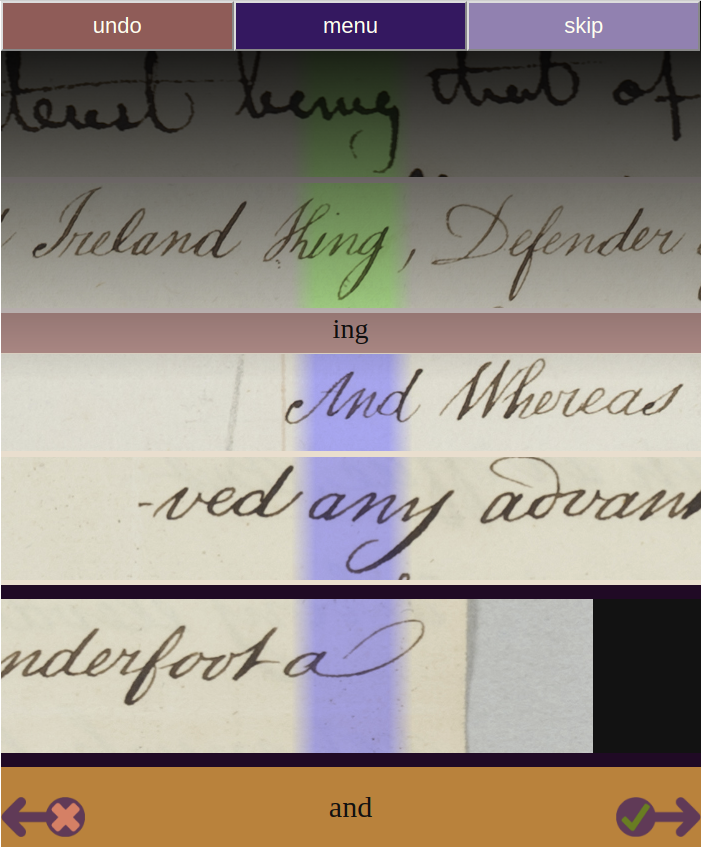
\includegraphics[width=.75\textwidth]{spottingapproval}
    \caption{Spotting approval UI. Instance being classified is at the bottom of the interface (dark border). The desired label ``and'' is below it. The next label ``ing'' can be seen above it with its associated instances above it.
    }
    \label{fig:spottingapproval}
\end{figure}

%%%%%%%%%%%%%%
\iffalse
Two modes were developed and tested: a swipe interface and a tap interface. We

\paragraph{Tap}
In this mode, a batch of 5 spottings were shown together (Figure \ref{im:?}). The user tapped on any incorrect spottings, and then tapped a submit button, after which another batch would be shown. This means that a user can potentially use one action to complete 5 spottings, though it may take 6 actions in the worse case.

\paragraph{Swipe}
In this mode, the spottings neededing approval queued in a stack with the desired character n-gram being shown at above the stack. see Figure \ref{im:?}. Users either swiped left or right to either reject or accept the spotting shown on the top of the stack. Unlike the tap mode, this forces users to make a decision about each n-gram, potentially increasing accuracy.


\paragraph{Evaluating Spotting Approval Modes}

fdsgfdh
\fi
%%%%%%%%%%%%%

\subsubsection{Transcription Selection}\label{transtask}
This task's interface can be seen in Figure \ref{fig:transcriptionselection}.
The user is presented with the image of the word with the spotted n-grams hilighted. Below are the n-gram labels each with an `x' button so the user can indicate an incorrect spotting.
Below these is the list of possible transcriptions. They are presented in an order according to their word spotting score, as this frequently places the correct transcription at the top.
At the end of this list an additional ``Error'' button allows the user to indicate that the correct transcription is not present, and the spotting n-grams are correct.

\begin{figure}
    \centering
    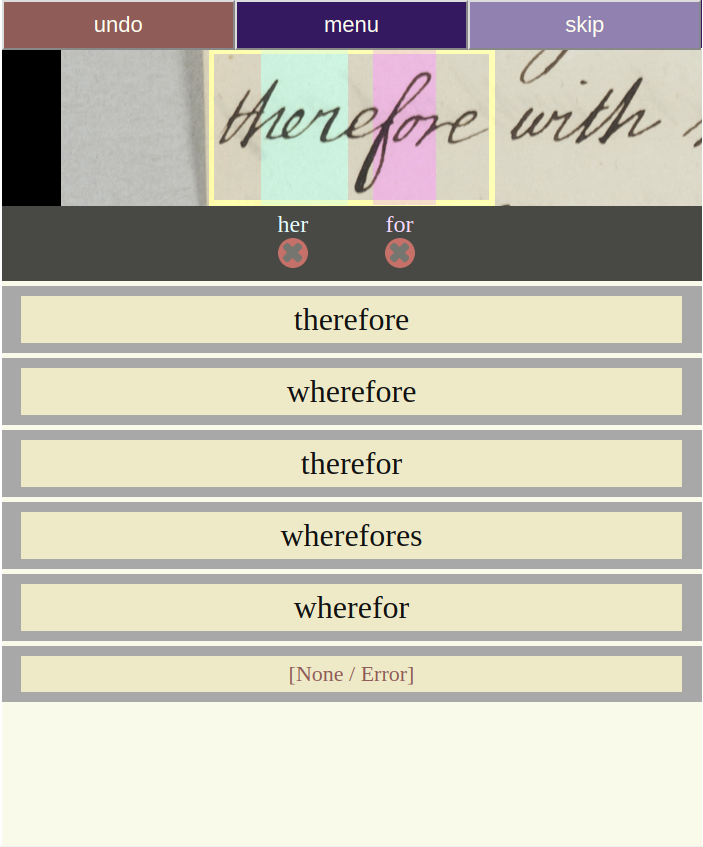
\includegraphics[width=.75\textwidth]{transcriptionselection}
    \caption{Transcription selection UI.  Both ``her'' and ``for'' have been spotted in the image. The user can remove spottings if they are incorrect (red `x's). The possible transcriptions are ordered according to their word spotting score; in many instances this puts the correct transcription at the top of the list.
    }
    \label{fig:transcriptionselection}
\end{figure}

%\subsubsection{Manual Transcription}
%This task's interface can be seen in Figure \ref{fig:manualtranscription}.
%Some words will not be able to be reduced to a short list of possible transcriptions due to poor spotting or possibly errors. These transcriptions must be manually entered by the user. It seems useful to use any known spottings on the given word to provide an intelligent lexicon from which an auto-complete might be able to speed up transcription. However, we observed that generally the spottings were too poor for this assistance to be of much help.



\subsection{Word Completion / Regular Expression Generation}\label{wordcompletion}
We rely on the word image width, estimate character width, and the locations of confirmed spottings (spottings approved by user or threshold) in the word to estimate how many characters have not been spotted in a word. This allows a regular expression to be generated which represents all possible transcriptions of that word.

Spottings are estimated to be a width calculated using the process described in Section \ref{detirminewindowsize}, but without the clustering.
We average these as an approximation of the character width of an unknown character.

The procedure to create the regular expression is as follows. First we measure the number of pixels between each confirmed spotting and divide this by the estimated character width, providing an estimated number of characters $\epsilon$ (with fractional characters). The range of characters used in the expression is 
round($\epsilon-0.8$) to round($\epsilon+0.8$).
%0.8 subtracted and added to the count estimate, rounded.
 The first and last characters are similarly computed, using the beggining and end of the image boundaries as the previous and next spottings, but we additionaly allow each of those ranges to have one less character than the range computed to account for the fact that frequently first and last letters are longer than others (e.g.~capital letters at the beginning of a word, or a long tail on the last character of a word). If spottings overlap by less than 0.15 the estimated character width, we allow a character to possibly be between them. If spottings overlap and share boundary characters (e.g.~`al' and `le' sharing `l') we permit either a double letter (`alle') or single (`ale') as the spotting methods we use would have trouble distinguishing these situations. 
 %Pseudo code is shown in Algorithm \ref{regex}.

%%%%Should be in appendix ?
%\begin{algorithm}\label{regex}
% \KwData{Word image width: $W$, List of spottings in word image: $S$ (where $S_i^L$ and $S_i^R$ are the leftmost and rightmost boundary of the $i$th spotting for a word and $S_i^T$ is the n-gram of the spotting), Estimate character width: $C$}
% \KwResult{regular expression for possible transcriptions}
% $i$:=$0$\;
% $p$:=$0$\;
% $r$:=`` ''; (return string)\\
% \While{$i < \text{length of }S$}{
% 
%  $\delta$:=$S_i^L - p$\;
%  $\epsilon$:=$\delta / C$; (estimated number of characters as a float)\\
%  
%  \eIf{$\epsilon > 0$}{
%   $l$:=$\text{floor}(\epsilon)$\;
%   $m$:=$\text{ceiling}(\epsilon)$\;
%   \If{$\epsilon - l < 0.3$ and $l>0$}{
%     $l$:=$l-1$\;
%   }
%   \If{$m - \epsilon < 0.3$}{
%     $m$:=$m+1$\;
%   }
%   $r$=$r$..``[a-zA-Z0-9]\{$l$,$m$\}''\;
%   }{
%   (Handling possible overlaps)\\
%   $o$:=$\text{length of }S_i^T$\;
%   \While{$o>0$}{
%     ....\;
%     $o$:=$o+1$\;
%   }
%  }
% }
% \caption{Regular expression generation from spottings.}
%\end{algorithm}



Once we have the regular expression, we find all matches in our lexicon.

If there are no matches there are three possible scenarios: the word is not in the lexicon, there is an incorrectly approved spotting, or the spottings and unlabeled characters' count or alignment didn't transfer to the regular expression properly.
To account for the second scenario, we iteratively try removing individual spottings, regenerating the regular expression, and requerying the lexicon to see if matches are found. We make the assumption that only one spotting will be incorrect and union the matching lexicon results. We first only remove spottings that have no overlap (overlap meaning two or more spottings idetified a mutual character) and then those that do.
If this fails to yield any lexicon matches, we try to account for the third scenario by regenerating the regular expression in a ``loose'' mode, where each range of unknown characters is expanded by one to allow matches initailly constrained by a bad aligment estimation.
If there are no matches and we are already using the ``loose'' regular expression we simply skip the word. It will be manually transcribed eventually.

If there are matches, and less than 49 of them, we score each possible transcription against the image using word spotting.
%That is, we word spot the possible transcription and the word spotting score is used.
As the possible transcriptions are based only on the regular expression, some will be obviously wrong from a visual point of view (e.g.~missing descenders). Following this intuition, we perform an Otsu threshold on the scores to attempt to discard the obviously wrong possibilties. This thresholding is only applied if there are more than 5 possibilities, or if the threshold falls less than half distance between the highest and lowest score (we're confident we're discarding something poor).
If the resulting number of possible transcriptions is less than 7, we package them into a transcription selection task, ordered by spotting score, and enqueue it for a user to complete.


\subsection{Receiving Transcription}
The user either returns a transcription selection task in three ways: with a selected transcription, with a spotting marked for removal, or with a error indication (see Section \ref{transtask}). These are handeled in the following ways.

If a transcription was selected, that is stored as the transcription for the word. We attempted to extract new ngram image exemplars by interpolating where unspotted n-grams were in the word image, but these generally failed to be good exemplars so we choose not to use them.

If a spotting is marked for removal, it is removed and the process described in Section \ref{wordcompletion} is followed again, potentailly leading to a new task being enqueued.

If the user indicates an error we first attempt to loosen the regular expression, as described in Section \ref{wordcompletion}. If no matching words are found, we remove the ``worst'' spotting. ``Worst'' first being any spotting labeled by a threshold (not user oversight), and then simply follows the spotting scores.


\subsection{Batch Distribution}
When approving spottings it is a non-trivial task to distribute the spottings to users in an efficient manner. We would like to maximize the humans efforts, ideally quickly finding thresholds for each n-gram that can be used to automatically label the remaining spottings. We tried several approaches to this.

The simplest method is to simply take the spotting with the highest score until the user begins to classify enough as false that  a we can assume we are at a good thresholding location to reject the remaining spottings. 
%In our implementation we make this decision after a running average of true classifications falls below 0.3, where the window is X. 
This has the downside of not looking for a possible threshold to accept spottings by and did not yield satisfactory results.




Looking at a graph of true and false spotting instances in Figure \ref{fig:two_dist_ex}, one can see that each of the groups forms a distintive distribution. If we can model these it would give us a useful tool to create both an accept and reject threshold. However, it is not always easy to do so. In Figure \ref{fig:one_dist_ex} we see that the false spottings almost subsumes the true spottings making them difficult to distinguish. We thus allow it to model the spottings either as two distributions or one.

\begin{figure}
    \centering
    \includegraphics[width=.75\textwidth]{two_dist_ex}
    \caption{A histogram of spotting instances for the bigram ``nd'' divided into true and false spottings. The true spottings forms a distribution distinct from the false.
    }
    \label{fig:two_dist_ex}
\end{figure}
\begin{figure}
    \centering
    \includegraphics[width=.75\textwidth]{one_dist_ex}
    \caption{A histogram of spotting instances for the unigram ``g'' divided into true and false spottings. The true spottings are almost inline with the false distribution making them indistinguishable.
    }
    \label{fig:one_dist_ex}
\end{figure}

We model the distributions as normal distributions, the false spottings being only half of the distribution (as we discard the worst scores for effiency).

When begining, we do a check to see whether we will model the spotting scores as one or two distributions. We model the scores as a single distrubution the see if there are large amount of outlier instances at it's ``tail'' (Figure \ref{fig:tail_dist_ex} green circle). This should be a distictive true distribution is present. We measure this by the difference between the probability density of the model and actual density of scores in the tail of the distrubution. The ``tail'' is defined by a threshold density.

\begin{figure}
    \centering
    \includegraphics[width=.75\textwidth]{tail_dist_ex}
    \caption{A histogram of spotting instances for the bigram ``nd'' with a curve (red) representing the data as a single distribution. The green circle shows that the estimation greatly underestimates the tail indicating there is likely a strong true instance distribution present.
    }
    \label{fig:tail_dist_ex}
\end{figure}

If we select two distributions, we estimate an initial split between true and false scores using the Otsu threshold. We model the two distributions assuming all spottings is true or false based on this threshold.

The distributions are constantly modeled using expectation maximization, an iteration of it being applied each time a batch is recieved. If a user label isn't known for a score, it's class is estimated using the current model.



For single distribution mode:
The accept threshold is the top score (i.e.~none).
The reject threshold is the end of the ``tail'' (density threshold on estimated distribution).

For dual distribution mode:
The accept threshold is a certain density threshold on the estimated true distribution.
The reject threshold is where the densities of the two distributions cross after the accept threshold.

This method is a bit fragile and can behave badly, particularly when it poorly models the true distribution in the two distribution scenario. There are several additional things to smooth its behavoir: 
There is are max accept and reject thresholds based on the current model of the false scores.
Reject threshold is brought to be closer to accept threshold.
The accept threshold is  shifted towards the better scores according to a runnning average of true classifications by users falls below 0.5.
For the single distribution the reject threshold is similarly shifted.
If the reject and accept threshold end up on the wrong side of eachother, the accept threshold is put at the top score and the reject threshold is set a number of instances down the sorted score list, the number being dependent on the running true classification average.

When creating a new batch, scores are sampled from a uniform distribution between the accept and reject thresholds and the closest unlabeled spottings are placed in the batch.

We also test with only using the single or dual distributions and not trying to guess which one is better.

When there are no instances left between the reject and accept thresholds, the n-gram is finished. All instances above the accept threshold are accepted and all below the reject threshold are rejected.

%ordered list
%attempt to find thresholds to accept/reject
%uniform between thresholds
%
%checks if all batches in before sending last 12
%
%top, draw best score
%guass, draw scores from guassian dist (closest spottings)
%fancy-single, draw uniform dist between thresholds
%fancy

\subsection{Receiving Spotting Approvals}

Every 5 updates we recheck whether it would be better to model the data as one or two distributions.
As a hard rule, if we've had over 2 ``bad'' batches, we switch to a single distribution modeling.

We then perform an expectation maximization step including the new spotting labels.



%\subsubsection{Exemplar extraction}

\subsection{Alternate Mode: Don't Wait to Transcribe}
After word spotting lexicon look up (Section \ref{wordcompletion}), return top 7
sdtore others
lexicon lookup

when error on trans, just enqueue next batch


%%%%%%%%%%%%%%%%%%%%%%%%%%%%%%%


\section{CAT Through Approved Subword Spottings Using Clustering}

The approval of spottings is a bottle-neck for the previous transcription strategy. In \cite{Retsinas2015}, they sped up approval by clustering printed characters together and presenting the user with a composite of a cluster. While handwriting it too noisy to composite, we follow a similar method of clustering n-gram spottings together and presenting users with (part of) a cluster to approve or disapprove. Classifying a group of spottings which belong to the same class should take as long as a single instance, the catch is that we don't know if a group of spottings is all right or all wrong. It's likely our clustering is imperfect so that there is a mix. However, in the case where only a few instances in the cluster are outliers, they should be quickly identified by a user (see Figures \ref{fig:clustergood} and \ref{fig:clusterbad}). In the case where the cluster is totall mixed (50\%/50\%) one can classify each instance individually.% (see Figure ??).

In this transcription strategy we use the same method as above, but change how spotting batches are distrubuted and don't use QbE in the same way. We will desribe the steps of this process next.

\subsection{Clustering}

We first perform a dense QbE comparison for the results of each initail n-gram QbS spotting. This gives us a similarity for all instances. We then perform a hierarchical complete-linkage agglomerative clustering (two clusters are merged if their two most dissimlar spottings are more similar than any other cluster pair). We choose a hierarchical method as this allows us to tune the ``purity'' of clusters as we recieve human feedback. ``Purity'' is the measure of how much the clusters are of one class ($2*max(T,F)/(T+F)-1$ where $T$ and $F$ are the count of true or false spottings in the cluseter). The initial level in the hierarchy is the first level where the average cluster size is above 10, which is roughly what we feel an ideal batch size is.



\begin{figure}
    \centering
    \includegraphics[width=0.8\textwidth]{clustergood2}
    \caption{The cluster spotting approval UI with a true cluster. One outlier has been identified by the user (darkened instance).}
    \label{fig:clustergood}
\end{figure}
\begin{figure}
    \centering
    \includegraphics[width=0.8\textwidth]{clusterbad}
    \caption{The cluster spotting approval UI with a false cluster. No outliers are present.}
    \label{fig:clusterbad}
\end{figure}

\subsection{Spotting Approval Batch Distribution}

We evaluated two methods of distributing clusters.
One simply takes the cluster with the next highest average score.
The other method attempts to identify good clusters based on their similarity to approved spottings. To do this we save each approved spotting in a queue. When finding a new cluster to distribute, we take the next instance off of the queue. We then find the cluster with that is closest using the complete-linkage metric, that is the cluster where the instance with the furthest distance from our exemplar is minimized.

In both methods, if a selected cluster is too large (maximum size of 15) we split it and send each piece as a seperate batch.

We have a goal ``purity'' of 0.9 (rougly 1 or 2 outliers per batch). When our moving average purity varies from this (over an $\epsilon$ threshold) we either move up a level in the heirarchy (we are too pure) or mode down a level in the heirarchy (we are not pure enough).

When our moving average accuracy (the portion of instances classified as true by the user) falls below a threshold (0.3) we stop sending batches for that n-gram.
%TODO test 0.4 threshold

\subsection{Spotting Approval UI}

Examples of the UI are shown in Figures \ref{fig:clustergood} and \ref{fig:clusterbad}. The idea is to allow the user to recognize whether the majority of the instances are correct or incorrect and then select the outliers. When a user selects an instance it is darkened. There are two buttons at the bottom which are used to both indicate the cluster type (correct/incorrect) and that they have selected all the outliers (they are finished).

This is a minimalist interface placing a fair amount of cognitive load onto the user in exchange for efficency. One can imagine a slightly simpiler interface where the cluster type is identified as a button prior to a ``done'' button.


%%%%

\section{CAT Through Unassisted Subword Spotting Using Dynamic Time-Warping Alignment} %

We want to avoid having to make decisions about spottings, either by thresholding or having user input, which the previous methods rely on. Thresholding forces a decision between recall and precision, and user input is costly. A way to avoid these is to simply merge all spottings together into a single character probability vector, resulting in something like Figure \ref{fig:cpv}, and then decode this.

\begin{figure}
    \centering
    \includegraphics[width=0.5\textwidth]{cpv}
    \caption{An example of a character probability vector for the word ``adultery''. The relative probability of each character (`a'-`z') at each horizontal position is represented both by the height and color of the graph. The discontinuities occuring at the begining and end of the word (e.g. see `x') occur due to the merging of unigram, bigram, and trigram scores.}
    \label{fig:cpv}
\end{figure}

The combining happens according to the following procedure.
We process each n (1, 2, and 3) seperately into an independent vector before combining them.

Each spotted n-gram produces a score at each location of the sliding window. For unigrams this gives us a vector for a relative scoring of a character at each location. For bigrams and trigrams we can offset these locations and create vectors for each character present in the bigram or trigram. These can them be summed together for a word image.
Each n-specific character vector is normalized according to how many n-grams contributed to that character.
We then perform a soft-max at each horizontal position over the characters. This is then slightly reduced if some letters did not contribute (no n-grams with that letter) to account for the soft-max being slightly higher on the letters which are present.

The individual n-specific vectors are summed and each letter normalized according to how many n-specific vectors contributed to it.
This summed result has another soft-max applied to it to yield the final character probability vector.

We then use dynamic time warping to score the character probability vectors agains the lexicon words, the lexicon words being one-hot vectors. Similar to the transcription via PHOC method we can then return the top 7 matches to the user to select the correct transcription.



%%%%%%%%%%%%%%%%%%%%%%%%%%%%%%%%%%%%%%%%

\chapter{Evaluation of Transcription Strategies}

In this chapter we will explain our procedure for testing the transcription strategies described in the previous chapter. Then we will examine the results of these tests.

\section{Evaluation Method}

We evaluate all our transcription strategies as CAT (computer assisted transcription) methods. However, rather than having users use the systems we simulate approximate user behavoir using collected statistics. While the statistics may not give results as accurate as a user study, it allows us to easily compare the performance of different transcription strategies using consistent timing data.

The statistics were collected from four reseachers
%, who were moderetly to tagently involved in this project, 
using the system. We collected timing information regarding how quickly they completed batches, whether they were correct (against the corpus ground truth and the author's judgement), as well as information regarding the batch's ``difficulty''. For spottings this was the size of the batch, the number of true instances, and whether the previous batch was the same n-gram. For transcription selection this was the position of the correct transcription (if present). 
%For manual transcription we recorded the length of the word(s). 
We fit linear models to predict the time needed to complete a batch based on its ``difficulty''. We also did this for errors.
We collected data for both spotting approval methods (instance and cluster).

In more detail, we measured which ``difficulty'' measure best modeled the data and used that. For transcription selection, there is a fixed time predicted if the correct transcription is not preset, otherwise a linear model based the transctions position in the list predicts time. Two fixed values predict the error the two transcription situations. 
%For manual transcription a linear model based on length predicts time and a fixed value predicts error (on the word level).  
For the Bentham dataset, instance spotting approval timing is based on whether the previous batch is the same n-gram. For the Census Names dataset, instance spotting approval timing is based on the number of true instances. For both datasets, error is based in the number of true instances in the batch. For both datasets, cluster spotting approval timing and error is based on the number of instances in the batch.

We also collected how long it took to manual transcribe line images so we can see if the CAT actually speeds up the transcription process.

To evaluate, we ran each strategy as a CAT system with a single simulated user. When the simulated user recieved a batch, it found the correct response and then measured the probabilty of error and introduced an error if a random value between [0,1] fell below that probability. The simulated user then computed the estimated time based on the appropriate model and waited that long before returning its answer. For many of the transcription strategies, there comes a point where the strategy must be abandon and the remaining words manual transcribed. We terminate our simulations at this point, but report how much was transcribed.

\section{Results}

We measure the speed of the transcriptions using a words-per-minute metric. This is averaged over the time of the system running, as it varies significantly during the running for the spotting approval method. The results are summarized on Table \ref{tab:finalresults}. In the following subsections we analyse the results of each method.

\begin{table}
\centering
\begin{tabular}{| l | c  c  c | c c c |}
  \hline
   & \multicolumn{3}{c|}{Bentham} & \multicolumn{3}{c|}{Census Names}\\
  Method & Transcribed & Words/Min & WER & Transcribed & Words/Min & WER\\
  %Method & Portion transcribed & Speed (w/m) & WER & Portion transcribed & Speed (w/m) & WER\\
%  \hline %old
%
%  Manual             & -   & 19.4 &  -   & 30.3?? \\
%  PHOC vectors 100\% & 0.845 & 19.9 &  0.669 & 22.8 \\
%  PHOC vectors 75\%  & 0.656 & 21.0 &  0.507 & 22.8 \\
%  PHOC vectors 50\%  & 0.437 & 20.9 &  0.393 & 28.5 \\
%  \hline	
%  \multicolumn{5}{|l|}{CAT through approved subword spottings} \\
%  Two-distributions B & 0.319 & 5.7 & 0.108 & 2.8 \\
%  Two-distributions UB & 0.453 & 5.2 & 0.206 & 4.1 \\
%  Closest cluster next B & 0.669 & 2.7 & 0.220 & 1.1 \\
%  \hline	
%  \multicolumn{5}{|l|}{CAT through unassisted subword spotting using DTW} \\
%  CPV+DTW UBT & 0.700 & 13.6 & 0.331 & 9.1 \\
  
  \hline		

  Manual             & -   & 24.27 & 0.927 &  -   & 20.92 & 0.840 \\
  PHOC vectors 100\% & 0.869 & 25.41 & 0.978 &  0.706 & 11.95 & 0.936 \\
  PHOC vectors 75\%  & 0.671 & 27.50 & 0.981 &  0.531 & 11.95 & 0.938 \\
  PHOC vectors 50\%  & 0.447 & 27.01 & 0.981 &  0.405 & 15.11 & 0.964 \\
  \hline	
  \multicolumn{7}{|l|}{CAT through approved subword spottings} \\
  Two-distributions B & 0.324 & 6.07 & 0.979 & 0.184 & 1.94 & 0.916 \\
  Two-distributions UB & 0.459 & 5.50 & 0.980 & 0.387 & 3.17 & 0.915 \\
  Closest cluster next B & 0.673 & 3.01 & 0.969 & 0.499 & 1.16 & 0.938 \\
  \hline	
  \multicolumn{7}{|l|}{CAT through unassisted subword spotting using DTW} \\
  CPV+DTW UBT & 0.738 & 15.52 & 0.955 & 0.391 & 5.05 & 0.822 \\
  %? & X & X & X & X \\
  \hline  
\end{tabular}
\caption{Highlights in the results from simulations. The letters U, B and T represent whether unigrams, bigrams and/or trigrams were used. The PHOC vector method is the only method we tested able to transcribe words at a rate faster than manual transcription.}
\label{tab:finalresults}
\end{table}

We note that all methods have better word-error-rate (WER) than manual. This is because all are aided by the lexicon. One can imagine that the manual transcription method could be augmented by showing users close lexical matches to the word a user is typing. This should make manual transcriptions WER comparable to the other methods at the cost of some speed as users now will spend some time looking at the lexical matches.


\subsection{CAT Through PHOC Vectors Results}
This baseline result is the only method to surpass manual transcription time, and it only did for the Bentham dataset. We show results in Table \ref{tab:finalresults} for three variations where the portion of words actually sent to the user is changed. As would be expected, decreasing the number of words sent to the user has a linear relationship with the portion transcribed, however, the speed does not follow this linear relationship. This simply means that the order of good transcription selection batches doesn't correlate directly to score.

We assume that the speed of this method on the Census Names dataset does not surpass manual due to the greater variation in the handwritting. Humans are typically better at handeling variation.

\subsection{CAT Through Approved Subword Spottings Results}

%We show the results of using the following combination of n-grams: bigrams alone, bigrams and trigrams, and unigrams, bigrams and trigrams. Bigrams alone far out performed unigrams or trigrams alone. Unigrams and trigrams only slightly underperforms bigrams and trigrams. %They both significantly outperform unigrams and bigrams. 
We show more detailed results in Table \ref{tab:appresults} for the following five variations of batch distribution: switch-distribution modeling, single-distribution modeling, two-distribution modeling, clusters returning the closest cluster next and clusters returning the highest scored cluster next. We also expirimented with other methods of distributing batches, however, these far outperformed the other approaches. We don't show an exhustive list of n-gram combinations, but show those that both cover a variety and were the best performing.

\begin{table}
\centering
\begin{tabular}{| l | c c c | c c c |}
  \hline
   & \multicolumn{3}{c|}{Bentham} & \multicolumn{3}{c|}{Census Names}\\
  Method & Transcribed & Words/Min & WER & Transcribed & Words/Min & WER\\
  %Method & Portion transcribed & Speed (w/m) & WER & Portion transcribed & Speed (w/m) & WER\\
%  \hline %old
%  Switch-distributions B & 0.324 & 5.3 &  0.098 & 2.2 \\
%  Switch-distributions BT & 0.504 & 3.0 &  0.185 & 1.6 \\
%  Switch-distributions UBT & 0.596 & 3.0 & 0.193 & 1.6 \\
%  Single-distributions B & 0.307 & 4.5 & 0.097 & 2.1 \\
%  Single-distributions BT & 0.512 & 2.8 & 0.185 & 1.6 \\
%  Single-distributions UBT & 0.597 & 2.7 & 0.192 & 1.5 \\
%  Two-distributions B & 0.319 & 5.7 & 0.108 & 2.8 \\
%  Two-distributions UB & 0.453 & 5.2 & 0.206 & 4.1 \\
%  Two-distributions BT & 0.498 & 3.8 & 0.181 & 2.1 \\
%  Two-distributions UBT & 0.594 & 3.6 & 0.265 & 2.8 \\
%  Closest cluster next B & 0.669 & 2.7 & 0.220 & 1.1 \\
%  Closest cluster next BT & 0.667& 2.7 & 0.220 & 1.1 \\
%  Closest cluster next UBT & 0.661 & 2.7 & 0.222 & 1.1 \\
%  Top cluster next B & 0.667 & 2.7 & 0.220 & 1.0 \\
%  Top cluster next BT & 0.671 & 2.7 & 0.222 & 1.1 \\
%  Top cluster next UBT & 0.657 & 2.7 & 0.220 & 1.0 \\
  \hline  
  Switch-distributions B & 0.329 & 5.39 & 0.957 &  0.195 & 1.74 & 0.906 \\
  Switch-distributions BT & 0.519 & 3.06 & 0.962 & 2.93 & 1.21 & 0.915  \\
  Switch-distributions UBT & 0.602 & 2.99 & 0.972 & 0.453 & 1.54 & 0.934 \\
  Single-distributions B & 0.312 & 4.72 & 0.971 & 0.188 & 1.56 & 0.912 \\
  Single-distributions BT & XX & XX & X & 0.301 & 1.13 & 0.922 \\
  Single-distributions UBT & 0.602 & 2.85 & 0.971 & 0.458 & 1.44 & 0.928 \\
  Two-distributions B & 0.324 & 6.07 & 0.979 & 0.184 & 1.94 & 0.916 \\
  Two-distributions UB & 0.459 & 5.50 & 0.980 & 0.387 & 3.17 & 0.915 \\
  Two-distributions BT & 0.504 & 3.68 & 0.952 & 0.261 & 1.41 & 0.922 \\
  Two-distributions UBT & 0.594 & 3.71 & 0.972 & 0.455 & 2.12 & 0.918 \\
  Closest cluster next B & 0.673 & 3.01 & 0.969 & 0.499 & 1.16 & 0.938 \\
  Closest cluster next BT & 0.670 & 2.80 & 0.969 & 0.500 & 1.16 & 0.932 \\
  Closest cluster next UBT & 0.669 & 2.78 & 0.968 & 0.500 & 1.16 & 0.935 \\
  Top cluster next B & 0.670 & 2.82 & 0.967 & 0.498 & 1.15 & 0.943 \\
  Top cluster next BT & 0.672 & 2.82 & 0.967 & 0.500 & 1.15 & 0.936 \\
  Top cluster next UBT & 0.675 & 2.81 & 0.969 & 0.502 & 1.16 & 0.929 \\
  \hline  
\end{tabular}
\caption{Results from simulations of CATTSS using user approval on subword spotting results. The letters U, B and T represent whether unigrams, bigrams and/or trigrams were used.}
\label{tab:appresults}
\end{table}

All of these methods perform far below manual transcription. In the best variation for the Bentham dataset (two-distributions with just bigrams) the simulated user spent 80\% of its time approving spottings. The effort required for the user to supervise the subword spotting represents a large slowdown to the system's speed. The Census Names dataset is consistently much slower than the Bentham dataset as the handwritting in it is more difficult and thus requires even more user supervision in approving subword spottings.

An part of a page of the testing corpus of the Bentham dataset is show in Figure \ref{fig:aftercattss} annotated with the spottings which were approved as well as the transcribed words.


\begin{figure}
    \centering
    \includegraphics[width=0.99\textwidth]{aftercattss}
    \caption{Part of a page of the Bentham dataset after running the CATTSS system with subword spotting approval being distributied using a two-distribution model with only bigrams. The pink boxes represent approved bigram spottings. The red text represents a transcription made by the system.}
    \label{fig:aftercattss}
\end{figure}




\subsection{CAT Through Unassisted Subword Spotting Using Dynamic Time-Warping Alignment Results}
%Fixes issue of spotting approval and is faster, but still not as good as PHOC-based.
%What is the difference between PHOC-based and DTW-based? Why is straight PHOC better? 

In the previous section we saw the subword spotting approval as a major bottleneck. We removed that bottleneck in this method by aggregating all spottings into character probability vectors and comparing these directly to our lexicon words using DTW. We see large gains doing this, but we still fail to beat manual transcription speeds by a wide margin. Details of the results can be seen in Table \ref{tab:dtwresults}. The best results used both unigrams, bigrams and trigrams; as the user does not have to approve any it makes sense that including more information would lead to better results.

Given the similarities between this method of using a character probability vector and the baseline method using PHOC vectors, we think it valuable to describe why this method preforms worse.
Both the PHOC vector approach and the subword spotting approach use the same network. The subword spotting approach attempts to create more localized information by evaluating the subwindows and using their location. However, PHOCNet uses a 5 level TPP layer and the PHOC vector has 5 levels as well; these provide a fair amount of resolution by themselves. Subword spotting introduces some ambiguity due to its poor localization. Some of this likely is present in the aggregated character probability vector and contributes to its worse behavoir. Additionally, the PHOCNet is trained on full word images, not subwindows. This means it will generally have better performance on word images, which the PHOC vector approach uses.

%Can you cut more corners to makes things faster but less accurate? yes, but we can to the same thing for PHOC-based trans
%Potentially viable method in absence of data-specific trained spotting method (A QbE model, but it would have to be really good).

\begin{table}
\centering
\begin{tabular}{| l | c c c | c c c |}
  \hline
   & \multicolumn{3}{c|}{Bentham} & \multicolumn{3}{c|}{Census Names}\\
  Method & Transcribed & Words/Min & WER & Transcribed & Words/Min & WER\\
  %Method & Portion transcribed & Speed (w/m) & Portion transcribed & Speed (w/m)\\
  %\hline %old
  %CPV+DTW B & 0.491 & 8.0 & 0.179 & 4.7 \\
  %CPV+DTW BT & 0.603 & 10.8 & 0.252 & 6.8 \\
  %CPV+DTW UB & 0.679 & 12.6 & 0.292 & 7.9 \\
  %CPV+DTW UBT & 0.700 & 13.6 & 0.331 & 9.1 \\
  \hline  
  CPV+DTW B & 0.539 & 8.55 & 0.916 & 0.252 & 2.99 & 0.683 \\
  CPV+DTW BT & 0.649 & 11.85 & 0.935 & 0.315 & 3.90 & 0.769 \\
  CPV+DTW UB & 0.717 & 13.96 & 0.954 & 0.356 & 4.49 & 0.796 \\
  CPV+DTW UBT & 0.738 & 15.52 & 0.955 & 0.391 & 5.05 & 0.822 \\
  \hline  
\end{tabular}
\caption{Results from simulations using character probability vectors derived from subword spotting resutls. The letters U, B and T represent whether unigrams, bigrams and/or trigrams were used.}
\label{tab:dtwresults}
\end{table}

%%%%%%%%%%%%%%%%%%%%%%%%%%%%%%%%%%%%%%%%%%%%%%%%%%%%%%%%%%%%%%%%%%%%%%%%%%%%%%


%%%%%%%%%%%%%%%%%%%%%%%%%%%%%%%%%%%%%%%%%%%%%%%%%%%%%%%%%%%%%%%%%%%%%%%%%%%%%%
%\chapter{System Testing and Results}

%blah blah

%%%%%%%%%%%%%%%%%%%%%%%%%%%%%%%%%%%%%%%%%%%%%%%%%%%%%%%%%%%%%%%%%%%%%%%%%%%%%%
\chapter{Conclusion}

In this thesis we have introduced subword spotting and a method of doing it leveraging state-of-the-art word spotting techniques. We have presented results of subword spotting at three granularities (uni-, bi- and trigrams) with two datasets and show it to be a more challenging task than word spotting. We showed three applications of subword spotting: manual trancription assisting, suffix spotting and CAT (computer assisted transcription).

We now summarize what we feel our contributions are with this work and then discuss potential future work.

\section{Contributions}

%1. Subword spotting evaluation
%2. Applications of subword spotting
%3. Transcription (RegEx, combining 1,2,3)
%4. Crowd source

Our primary contribution is the exploration of subword spotting, a previously unexamined area. We have shown that while word spotting has achieved good results with modern techniques, applying similar techniques to subword spotting does not yield as percise of results.
Some insights from our subword spotting experiments that we feel are important are that 
size estimation of subwords is important if using a sliding window
and that
the number of characters in a subword  and its frequency in the data set does not directly correlate with the precision one can spot it.

A further contribution is our exploration of a few applications of subword spotting.
We show how subword spotting can be used to assist people manually transcribing documents by helping locate instances of unknown characters. Subword spotting we feel is a good fit for this task as a person may want to search for a group of characters together, or may not even recognize where character boundaries are.
We evaluate the performance of subword spotting when applied to the task of suffix spotting. 
%This could easily be extended to include preffix spotting. 
These searches can achieve results not readily available with word spotting and, as discussed in the next section, can be extended to even more customizable searches.
We attempt to apply subword spotting to CAT, but fail to achieve usable results. However, the method has potential given adjustments discussed in the next section.


\section{Future Work}

%deslant
%segmentation free
%training free

%regex search/spotting
%CPV to regex

There are several things that could have improved the subword spotting. We did not perform any preprocessing. State-of-the-art word spotting methods do not deslant word images. However, for subword spotting, deslanting the word images could have made localization better as the character boundaries would be more defined. While we attempted to refine individual spotting results to improve score and localization, we did not have success. However, they may be a refinment method we did not try which would succeed.

Everything we did in this work was based on word segmentation. However, it would not be difficult to extend what we have done to a segmentation-free scenario. One would need to be able to distinguish the situation of letters having a space between them, but after this it should extended quite straightforwardly.

While we aggregated spottings into regular expressions, an extension of suffix spotting would be regular expression spotting. That is, the user supplies a regular expression and the system returns all word images which match the expression. With some work, subword spotting should be able to achieve this. One could spot all n-grams in the expression and then use the structure of the expression to aggregate the scores accroding to their spatial relationships.

Our CAT strategies were not successfull, and if they were they would need to be competitive with modern automatic handwriting recognition methods (CNN+RNN) to be applicable. However, there is a slightly different application our method has the potential to work in.
Both our spotting method (PHOCNet) and modern automatic handwriting recognition methods (CNN+RNN) require traning data from a corpus before they can begin to work effectively. In a real workflow this will be a part of the corpus that must be manually transcribed. However, given an effective QbE subword spotting method that does not require corpus specific training, the CATTSS methods described in Chapter \ref{transcription} should work with few adjustments. Rather than the system initailly spotting a set of n-grams, a user would need to crop a few from the corpus to seed the system. After this, however, it should be able to proceed as outlined in Chapter \ref{transcription}.
The key is that the untrained QbE spotting method must be better than the QbS spotting we have demonstrated. Currently such a method does not exist.


\chapter{Appendix}

\begin{table}
\centering
\begin{tabular}{| l | c c | c c |}
  \hline
  & \multicolumn{2}{c|}{Bentham} & \multicolumn{2}{c|}{Census Names}\\
   %& QbS & QbE & QbS & QbE \\
  n-gram & Spotting width & Predicted width & Spotting width & Predicted width \\
  \hline
  a & 38 & 48 & 20 & 20 \\
  b & 33 & 36 & 27 & 28 \\
  c & 30 & 36 & 42 & 60 \\
  d & 48 & 64 & 23 & 20 \\
  e & 34 & 48 & 17 & 20 \\
  f & 35 & 48 & 44 & 60 \\
  g & 38 & 48 & 33 & 40 \\
  h & 31 & 36 & 26 & 28 \\
  i & 26 & 36 & 16 & 20 \\
  j & 42 & 64 & 41 & 60 \\
  k & 48 & 64 & 28 & 28 \\
  l & 30 & 36 & 20 & 20 \\
  m & 58 & 64 & 28 & 20 \\
  n & 45 & 48 & 32 & 40 \\
  o & 31 & 36 & 24 & 28 \\
  p & 38 & 36 & 38 & 56 \\
  q & 57 & 76 & 40 & 56 \\
  r & 31 & 36 & 17 & 20 \\
  s & 36 & 48 & 21 & 20 \\
  t & 32 & 36 & 17 & 20 \\
  u & 39 & 48 & 20 & 20 \\
  v & 42 & 48 & 35 & 44 \\
  w & 53 & 64 & 39 & 44 \\
  x & 52 & 64 & 18 & 20 \\
  y & 44 & 64 & 30 & 40 \\
  z & 48 & 64 & 39 & 60 \\
  ac & 58 & 64 & 46 & 44 \\
  ad & 72 & 76 & 49 & 44 \\
  ai & 59 & 64 & 46 & 56 \\
  al & 59 & 64 & 44 & 44 \\
  an & 69 & 64 & 48 & 44 \\
  ar & 58 & 64 & 39 & 40 \\
  as & 60 & 64 & 51 & 56 \\
  at & 67 & 76 & 61 & 84 \\
  be & 66 & 76 & 50 & 56 \\
  ca & 58 & 64 & 60 & 72 \\
  ce & 62 & 76 & 42 & 44 \\
  ch & 55 & 64 & 61 & 72 \\
  co & 51 & 48 & 49 & 56 \\
  ct & 54 & 64 & 42 & 44 \\
  de & 68 & 76 & 33 & 20 \\
  di & 74 & 96 & 32 & 20 \\
  ea & 55 & 48 & 53 & 68 \\
  ec & 54 & 64 & 42 & 44 \\
  ed & 64 & 64 & 63 & 84 \\
  ee & 63 & 76 & 49 & 68 \\
  el & 67 & 84 & 54 & 72 \\
  em & 81 & 76 & 58 & 60 \\
  en & 61 & 64 & 50 & 56 \\
  er & 56 & 64 & 46 & 56 \\
  es & 48 & 48 & 29 & 20 \\
  et & 57 & 64 & 28 & 20 \\
  fo & 48 & 48 & 46 & 44 \\
  ge & 58 & 64 & 40 & 40 \\
  ha & 69 & 76 & 46 & 40 \\
  he & 49 & 48 & 40 & 40 \\
  hi & 63 & 76 & 31 & 20 \\
  ho & 58 & 64 & 41 & 40 \\
  ic & 60 & 76 & 53 & 68 \\
  ie & 39 & 36 & 26 & 20 \\
  il & 41 & 36 & 33 & 28 \\
  im & 61 & 48 & 45 & 40 \\
  in & 71 & 84 & 31 & 20 \\
  io & 49 & 48 & 37 & 40 \\
  is & 54 & 64 & 40 & 44 \\
  it & 61 & 76 & 57 & 84 \\
  la & 57 & 64 & 40 & 40 \\
  le & 55 & 64 & 36 & 40 \\
  li & 61 & 76 & 35 & 40 \\
  ll & 55 & 64 & 29 & 20 \\
  lo & 47 & 48 & 29 & 20 \\
  ly & 55 & 48 & 32 & 20 \\
  ma & 95 & 96 & 54 & 44 \\
  me & 83 & 84 & 42 & 28 \\
  mi & 93 & 108 & 43 & 28 \\
  mo & 89 & 96 & 39 & 20 \\
  na & 81 & 96 & 42 & 28 \\
  nc & 69 & 76 & 55 & 60 \\
  nd & 75 & 76 & 60 & 68 \\
  ne & 59 & 64 & 52 & 60 \\
  ng & 73 & 76 & 61 & 68 \\
  ni & 67 & 76 & 59 & 72 \\
  no & 70 & 76 & 47 & 44 \\
  ns & 63 & 64 & 42 & 40 \\
  nt & 73 & 84 & 51 & 56 \\
  of & 64 & 76 & 55 & 68 \\
  ol & 55 & 64 & 45 & 56 \\
  om & 77 & 76 & 39 & 20 \\
  on & 78 & 96 & 33 & 20 \\
  or & 56 & 64 & 29 & 20 \\
  ot & 59 & 64 & 37 & 40 \\
  ou & 66 & 76 & 40 & 40 \\
  ow & 84 & 96 & 59 & 68 \\
  pa & 75 & 76 & 48 & 44 \\
  pe & 69 & 76 & 61 & 84 \\
  po & 69 & 76 & 44 & 44 \\
  pr & 68 & 76 & 43 & 44 \\
  ra & 60 & 64 & 43 & 44 \\
  re & 44 & 36 & 28 & 20 \\
  ri & 58 & 64 & 27 & 20 \\
  ro & 52 & 48 & 33 & 28 \\
  rs & 57 & 64 & 34 & 28 \\
  rt & 54 & 64 & 28 & 20 \\
  se & 48 & 48 & 31 & 28 \\
  sh & 61 & 64 & 54 & 60 \\
  si & 54 & 64 & 56 & 72 \\
  so & 53 & 48 & 34 & 28 \\
  ss & 66 & 76 & 49 & 56 \\
  st & 64 & 76 & 30 & 20 \\
  ta & 55 & 48 & 39 & 40 \\
  te & 43 & 36 & 30 & 28 \\
  th & 57 & 64 & 43 & 40 \\
  ti & 59 & 76 & 35 & 40 \\
  to & 57 & 64 & 29 & 20 \\
  tr & 46 & 36 & 28 & 20 \\
  ts & 60 & 64 & 30 & 20 \\
  ul & 60 & 64 & 48 & 56 \\
  un & 80 & 84 & 56 & 60 \\
  ur & 53 & 48 & 47 & 56 \\
  us & 61 & 64 & 47 & 44 \\
  ut & 52 & 48 & 33 & 28 \\
  ve & 62 & 64 & 52 & 68 \\
  wa & 79 & 76 & 69 & 84 \\
  we & 75 & 76 & 52 & 56 \\
  wh & 76 & 76 & 57 & 56 \\
  wi & 75 & 84 & 59 & 68 \\
  abl & 102 & 120 & 55 & 40 \\
  abo & 85 & 76 & 69 & 68 \\
  ace & 73 & 64 & 65 & 68 \\
  ach & 75 & 64 & 69 & 68 \\
  act & 89 & 96 & 66 & 68 \\
  ade & 87 & 76 & 70 & 68 \\
  age & 89 & 84 & 54 & 40 \\
  ain & 88 & 84 & 57 & 44 \\
  ake & 85 & 76 & 76 & 84 \\
  ali & 109 & 140 & 49 & 40 \\
  all & 89 & 96 & 57 & 56 \\
  als & 79 & 76 & 65 & 68 \\
  ame & 111 & 108 & 68 & 56 \\
  anc & 99 & 108 & 73 & 72 \\
  and & 111 & 120 & 80 & 84 \\
  ang & 87 & 76 & 75 & 72 \\
  ans & 93 & 84 & 82 & 84 \\
  ant & 96 & 96 & 65 & 60 \\
  any & 118 & 140 & 73 & 72 \\
  app & 101 & 96 & 71 & 72 \\
  ard & 94 & 96 & 62 & 56 \\
  are & 92 & 96 & 56 & 56 \\
  ari & 74 & 64 & 49 & 40 \\
  art & 78 & 76 & 62 & 68 \\
  ary & 94 & 96 & 75 & 84 \\
  ase & 81 & 76 & 64 & 68 \\
  ass & 92 & 96 & 65 & 68 \\
  ast & 89 & 96 & 64 & 68 \\
  ate & 89 & 96 & 61 & 60 \\
  ati & 89 & 96 & 60 & 60 \\
  att & 73 & 64 & 66 & 72 \\
  ave & 87 & 84 & 66 & 68 \\
  ber & 75 & 64 & 77 & 84 \\
  ble & 90 & 96 & 81 & 100 \\
  but & 115 & 140 & 68 & 68 \\
  cal & 73 & 64 & 67 & 68 \\
  can & 107 & 120 & 73 & 72 \\
  cat & 73 & 64 & 66 & 68 \\
  cen & 89 & 96 & 84 & 100 \\
  ces & 84 & 96 & 63 & 68 \\
  cha & 113 & 140 & 75 & 72 \\
  che & 75 & 76 & 54 & 40 \\
  chi & 85 & 96 & 66 & 68 \\
  cia & 89 & 96 & 64 & 68 \\
  com & 111 & 120 & 78 & 72 \\
  con & 86 & 84 & 69 & 68 \\
  cou & 74 & 64 & 67 & 68 \\
  cti & 87 & 108 & 59 & 60 \\
  ded & 94 & 96 & 73 & 72 \\
  den & 81 & 64 & 61 & 44 \\
  der & 82 & 76 & 56 & 44 \\
  des & 82 & 76 & 67 & 68 \\
  din & 91 & 84 & 70 & 68 \\
  dis & 84 & 84 & 66 & 68 \\
  duc & 95 & 96 & 74 & 72 \\
  ead & 89 & 84 & 70 & 68 \\
  ear & 76 & 64 & 54 & 44 \\
  eas & 79 & 76 & 64 & 68 \\
  eat & 75 & 64 & 56 & 56 \\
  eco & 77 & 76 & 61 & 60 \\
  ect & 81 & 84 & 61 & 60 \\
  een & 118 & 140 & 59 & 56 \\
  eir & 68 & 64 & 55 & 60 \\
  ell & 103 & 140 & 48 & 40 \\
  ely & 85 & 84 & 62 & 68 \\
  eme & 115 & 120 & 72 & 72 \\
  enc & 91 & 96 & 70 & 72 \\
  end & 101 & 108 & 72 & 72 \\
  ene & 80 & 76 & 59 & 56 \\
  ens & 81 & 76 & 69 & 72 \\
  ent & 102 & 120 & 64 & 68 \\
  era & 84 & 84 & 61 & 60 \\
  ere & 76 & 76 & 46 & 40 \\
  eri & 88 & 108 & 59 & 68 \\
  ern & 113 & 140 & 77 & 84 \\
  ers & 78 & 76 & 54 & 56 \\
  ert & 80 & 84 & 53 & 56 \\
  ery & 84 & 84 & 61 & 60 \\
  ese & 73 & 64 & 58 & 60 \\
  ess & 120 & 164 & 60 & 60 \\
  est & 77 & 76 & 50 & 44 \\
  eve & 85 & 84 & 78 & 100 \\
  exp & 111 & 120 & 62 & 68 \\
  fer & 75 & 76 & 64 & 68 \\
  ffe & 71 & 64 & 70 & 68 \\
  fic & 88 & 108 & 66 & 68 \\
  for & 78 & 76 & 52 & 40 \\
  fro & 84 & 84 & 65 & 68 \\
  gen & 93 & 96 & 70 & 68 \\
  ght & 89 & 96 & 72 & 72 \\
  gra & 78 & 64 & 68 & 68 \\
  gre & 86 & 84 & 63 & 68 \\
  had & 81 & 64 & 77 & 72 \\
  han & 108 & 120 & 76 & 72 \\
  har & 85 & 76 & 55 & 40 \\
  has & 111 & 140 & 71 & 72 \\
  hat & 94 & 96 & 69 & 68 \\
  hav & 105 & 120 & 72 & 72 \\
  hea & 88 & 84 & 54 & 40 \\
  hei & 88 & 96 & 61 & 60 \\
  hem & 116 & 120 & 79 & 72 \\
  hen & 88 & 84 & 56 & 40 \\
  her & 83 & 84 & 55 & 44 \\
  hes & 99 & 120 & 53 & 40 \\
  hey & 98 & 108 & 68 & 68 \\
  hic & 71 & 64 & 66 & 68 \\
  hin & 78 & 64 & 55 & 40 \\
  his & 81 & 84 & 64 & 68 \\
  hou & 97 & 108 & 70 & 68 \\
  how & 101 & 96 & 77 & 72 \\
  ial & 77 & 76 & 61 & 60 \\
  ica & 75 & 76 & 64 & 68 \\
  ice & 67 & 64 & 68 & 84 \\
  ich & 75 & 76 & 83 & 100 \\
  ide & 75 & 64 & 63 & 68 \\
  ien & 74 & 64 & 50 & 40 \\
  ies & 75 & 76 & 57 & 60 \\
  igh & 73 & 64 & 62 & 56 \\
  ill & 77 & 84 & 77 & 100 \\
  ime & 97 & 96 & 70 & 68 \\
  imp & 101 & 84 & 76 & 72 \\
  ina & 90 & 84 & 65 & 68 \\
  inc & 77 & 76 & 59 & 56 \\
  ind & 93 & 96 & 68 & 68 \\
  ine & 78 & 76 & 72 & 84 \\
  ing & 87 & 84 & 54 & 40 \\
  ini & 72 & 64 & 57 & 56 \\
  ins & 77 & 64 & 70 & 72 \\
  int & 86 & 84 & 72 & 84 \\
  ion & 90 & 96 & 63 & 68 \\
  ire & 82 & 96 & 55 & 60 \\
  ish & 75 & 76 & 64 & 68 \\
  ist & 69 & 64 & 58 & 60 \\
  ite & 73 & 76 & 55 & 60 \\
  ith & 88 & 96 & 68 & 72 \\
  iti & 65 & 64 & 70 & 84 \\
  its & 75 & 76 & 58 & 60 \\
  ity & 81 & 84 & 60 & 60 \\
  ive & 87 & 96 & 47 & 40 \\
  kin & 109 & 120 & 67 & 68 \\
  lan & 86 & 76 & 63 & 56 \\
  lar & 74 & 64 & 73 & 84 \\
  lat & 77 & 76 & 51 & 40 \\
  lea & 79 & 76 & 80 & 100 \\
  led & 75 & 64 & 57 & 44 \\
  les & 87 & 96 & 59 & 60 \\
  lic & 67 & 64 & 79 & 100 \\
  lin & 94 & 108 & 51 & 40 \\
  lit & 87 & 108 & 56 & 60 \\
  lle & 97 & 120 & 54 & 56 \\
  lly & 91 & 96 & 64 & 68 \\
  low & 108 & 120 & 86 & 100 \\
  man & 124 & 120 & 89 & 84 \\
  mar & 98 & 76 & 78 & 72 \\
  mat & 107 & 96 & 78 & 72 \\
  men & 122 & 120 & 79 & 72 \\
  mer & 92 & 76 & 81 & 84 \\
  min & 100 & 84 & 83 & 84 \\
  mon & 122 & 120 & 85 & 84 \\
  mor & 115 & 120 & 74 & 72 \\
  mpl & 133 & 140 & 79 & 72 \\
  nal & 98 & 96 & 79 & 84 \\
  nat & 102 & 108 & 69 & 68 \\
  nce & 77 & 64 & 62 & 56 \\
  nde & 105 & 108 & 85 & 100 \\
  ndi & 119 & 140 & 70 & 68 \\
  ned & 95 & 96 & 72 & 72 \\
  ner & 93 & 96 & 73 & 84 \\
  nes & 85 & 76 & 61 & 56 \\
  nge & 85 & 76 & 70 & 68 \\
  nin & 106 & 120 & 55 & 40 \\
  not & 116 & 140 & 65 & 68 \\
  now & 135 & 164 & 82 & 84 \\
  nsi & 89 & 96 & 64 & 68 \\
  nst & 95 & 96 & 67 & 68 \\
  nta & 92 & 84 & 69 & 68 \\
  nte & 82 & 76 & 81 & 100 \\
  nti & 86 & 84 & 62 & 68 \\
  ntr & 81 & 76 & 64 & 68 \\
  nts & 99 & 108 & 67 & 68 \\
  ome & 106 & 108 & 73 & 72 \\
  omm & 154 & 164 & 90 & 84 \\
  omp & 126 & 140 & 71 & 60 \\
  ona & 106 & 120 & 63 & 56 \\
  ond & 88 & 76 & 73 & 72 \\
  one & 82 & 76 & 74 & 84 \\
  ong & 94 & 96 & 71 & 72 \\
  ons & 90 & 84 & 67 & 68 \\
  ont & 82 & 76 & 66 & 68 \\
  ope & 76 & 64 & 72 & 84 \\
  ord & 88 & 84 & 59 & 56 \\
  ore & 77 & 76 & 51 & 44 \\
  orm & 131 & 164 & 74 & 72 \\
  ort & 87 & 96 & 58 & 60 \\
  ose & 87 & 96 & 49 & 40 \\
  ost & 109 & 140 & 71 & 84 \\
  oth & 78 & 76 & 70 & 72 \\
  oug & 88 & 84 & 71 & 72 \\
  oul & 87 & 84 & 64 & 68 \\
  oun & 87 & 76 & 65 & 60 \\
  our & 88 & 84 & 63 & 68 \\
  ous & 86 & 84 & 60 & 56 \\
  out & 91 & 96 & 63 & 68 \\
  ove & 73 & 64 & 61 & 60 \\
  owe & 106 & 120 & 69 & 68 \\
  own & 115 & 120 & 74 & 68 \\
  par & 92 & 84 & 67 & 68 \\
  pec & 97 & 108 & 65 & 68 \\
  per & 88 & 84 & 76 & 84 \\
  pla & 93 & 96 & 67 & 68 \\
  ple & 81 & 76 & 80 & 100 \\
  por & 99 & 108 & 63 & 68 \\
  pos & 91 & 96 & 65 & 68 \\
  pre & 90 & 96 & 61 & 60 \\
  pri & 102 & 120 & 60 & 60 \\
  pro & 101 & 108 & 63 & 68 \\
  rac & 82 & 76 & 66 & 68 \\
  ral & 92 & 96 & 63 & 68 \\
  ran & 97 & 96 & 61 & 56 \\
  rat & 92 & 96 & 62 & 68 \\
  rea & 84 & 84 & 58 & 56 \\
  rec & 84 & 96 & 61 & 60 \\
  red & 86 & 84 & 74 & 84 \\
  ree & 88 & 96 & 46 & 40 \\
  rel & 82 & 84 & 67 & 84 \\
  ren & 77 & 64 & 51 & 40 \\
  res & 78 & 76 & 52 & 44 \\
  ric & 84 & 96 & 56 & 56 \\
  rie & 72 & 76 & 53 & 56 \\
  rin & 123 & 164 & 50 & 40 \\
  ris & 100 & 120 & 55 & 56 \\
  rit & 96 & 120 & 52 & 56 \\
  rom & 125 & 140 & 74 & 72 \\
  rou & 88 & 84 & 63 & 68 \\
  rti & 68 & 64 & 55 & 60 \\
  sed & 86 & 84 & 67 & 68 \\
  see & 83 & 84 & 58 & 60 \\
  sel & 73 & 64 & 79 & 100 \\
  sen & 81 & 76 & 83 & 100 \\
  ser & 80 & 76 & 59 & 60 \\
  ses & 76 & 76 & 61 & 60 \\
  she & 79 & 76 & 66 & 68 \\
  sho & 98 & 108 & 67 & 68 \\
  sin & 89 & 96 & 64 & 68 \\
  sio & 91 & 108 & 58 & 60 \\
  sit & 69 & 64 & 58 & 60 \\
  som & 103 & 96 & 76 & 72 \\
  son & 84 & 76 & 70 & 72 \\
  spe & 83 & 76 & 64 & 68 \\
  sse & 100 & 120 & 61 & 60 \\
  ssi & 88 & 96 & 65 & 72 \\
  sta & 81 & 76 & 64 & 68 \\
  ste & 75 & 76 & 48 & 40 \\
  sti & 87 & 96 & 58 & 60 \\
  sto & 71 & 64 & 55 & 56 \\
  str & 72 & 64 & 60 & 60 \\
  sur & 83 & 76 & 64 & 68 \\
  tai & 85 & 96 & 60 & 60 \\
  tal & 81 & 76 & 51 & 40 \\
  tan & 86 & 76 & 69 & 68 \\
  tat & 73 & 64 & 62 & 68 \\
  ted & 85 & 84 & 65 & 68 \\
  ten & 76 & 64 & 64 & 68 \\
  ter & 76 & 76 & 55 & 56 \\
  tes & 77 & 76 & 59 & 60 \\
  tha & 86 & 84 & 65 & 60 \\
  the & 84 & 84 & 81 & 100 \\
  thi & 78 & 76 & 62 & 68 \\
  tho & 80 & 76 & 65 & 68 \\
  tic & 73 & 76 & 59 & 60 \\
  tim & 93 & 84 & 71 & 72 \\
  tin & 88 & 96 & 52 & 44 \\
  tio & 68 & 64 & 56 & 60 \\
  tiv & 97 & 120 & 58 & 60 \\
  tor & 83 & 84 & 58 & 60 \\
  tra & 80 & 76 & 62 & 68 \\
  tri & 84 & 96 & 46 & 40 \\
  tte & 69 & 64 & 55 & 56 \\
  tur & 79 & 76 & 62 & 68 \\
  ual & 88 & 84 & 67 & 68 \\
  uch & 128 & 164 & 73 & 72 \\
  ugh & 96 & 96 & 59 & 40 \\
  uld & 90 & 84 & 71 & 72 \\
  und & 106 & 108 & 77 & 72 \\
  uni & 93 & 96 & 67 & 68 \\
  unt & 91 & 84 & 67 & 68 \\
  ure & 81 & 76 & 61 & 60 \\
  use & 78 & 64 & 64 & 68 \\
  ust & 82 & 76 & 60 & 56 \\
  ven & 97 & 96 & 83 & 100 \\
  ver & 88 & 96 & 57 & 56 \\
  was & 99 & 96 & 76 & 72 \\
  wer & 99 & 96 & 69 & 68 \\
  whe & 88 & 76 & 76 & 72 \\
  whi & 106 & 120 & 74 & 72 \\
  who & 109 & 120 & 77 & 72 \\
  wil & 112 & 140 & 68 & 68 \\
  wit & 100 & 108 & 67 & 68 \\
  wor & 99 & 96 & 70 & 68 \\
  you & 131 & 164 & 67 & 68 \\
  \hline 
\end{tabular}
\caption{Optimal sliding window widths for spotting and estimated visual widths for each n-gram of interest.}
\label{tab:customwidths}
\end{table}


%\nocite{testentry}

\bibliographystyle{plainnat}
\bibliography{bib}

\end{document}

% vim: lbr
